\documentclass[11pt]{article}
\renewcommand{\baselinestretch}{1.2} 
\newcommand{\paragraphAndNewLine}[1]{\paragraph{#1}\mbox{}\\}
\usepackage[utf8]{inputenc}
\usepackage[T1]{fontenc}
\usepackage{graphicx}
\graphicspath{ {./images/} }
\usepackage{longtable}
\usepackage{float}
\usepackage{wrapfig}
\usepackage{rotating}
\usepackage[normalem]{ulem}
\usepackage{amsmath}
\usepackage{textcomp}
\usepackage{marvosym}
\usepackage{wasysym}
\usepackage{amssymb}
\usepackage{hyperref}
\usepackage{cite}
\usepackage{hyperref}
\usepackage{amsthm}
\usepackage{tabularx}
\usepackage{subcaption}
\usepackage{enumitem}
\usepackage[nottoc]{tocbibind}
\usepackage{tikz}
\usepackage{tkz-euclide}
\usetikzlibrary{calc,intersections}
\usetikzlibrary{arrows}
\usetikzlibrary{through}
\usetkzobj{all}

% make the proof label bold
\makeatletter
\renewenvironment{proof}[1][\proofname]{
   \par\pushQED{\qed}\normalfont
   \topsep6\p@\@plus6\p@\relax
   \trivlist\item[\hskip\labelsep\bfseries#1\@addpunct{.}]
   \ignorespaces
}{
   \popQED\endtrivlist\@endpefalse
}
\makeatother

\numberwithin{equation}{section}
\newcolumntype{L}[1]{>{\raggedright\arraybackslash}p{#1}}

\def\OZ{\Omega_{\zeta}}
\def\AZT{A^{\zeta}(t)}
\def\AZN{A^{\zeta}(n)}
\def\MZT{M^{\zeta}(t)}
\def\MZDOT{M^{\zeta}(\cdot)}
\def\Ex{\mathbb{E}}
\def\FS{\mathcal{F}_s}
\def\FT{\mathcal{F}_t}
\def\QVT{\langle M^{\zeta} \rangle_t}
\def\QV{\langle M ^{\zeta} \rangle}
\def\TFLOOR{\left \lfloor{t}\right \rfloor}
\def\TCEIL{\left \lceil{t}\right \rceil}
\def\EMT{\mathcal{E}^{m}(t)}
\def\LLT{\mathcal{L}^{l}(t)}
\def\indicator{\boldsymbol{1}}
\def\mydot{\boldsymbol{\cdot}}

\tolerance=1000

\newtheorem{theorem}{Theorem}
\newtheorem{lemma}[theorem]{Lemma} 
\newtheorem{corollary}[theorem]{Corollary}
\newtheorem*{remark}{Remark}

\begin{document}
\begin{titlepage}
  \centering
  \par\vspace{1cm}{\LARGE Universität Leipzig \par}
  \vspace {0.3cm}
  {\Large Fakultät für Mathematik und Informatik\par}
  \vspace {0.3cm}
  {\Large Mathematisches Institut \par}     
  \vspace {2.0cm}
  {\huge\bfseries Logarithmic Fluctuations for Internal DLA
   and Grid Brownian Motions
   \par}
  \vspace {5.0cm}
  {\scshape\Large Diplomarbeit \par}
  \vspace {0.6cm}
  { vorgelegt von \par}
  \vspace {0.6cm}
  { \large Lennart Johannes Clausen \par}
  \vspace {0.6cm}
  { am 05.05.2020
  \par}
  \vspace {0.6cm}
  {Betreuer \par}
  \vspace{0.6cm}
  {Prof. Artem Sapozhnikov\par}
  \vfill
\end{titlepage}

\thispagestyle{empty}
\begin{center}
  \vspace{1cm} 
  \hspace{10pt}
  \begin{abstract}
    In my thesis I consider internal diffusion limited aggregation—a random growth model—on 
    the two-dimensional lattice.    
    With each step, a new particle starts in the origin and performs a random walk 
    until it hits an unoccupied lattice point, where it stops.   
    I am interested in the asymptotic growth of the occupied cluster. 
    Lawler, Bramson, and Griffeath \cite{lawler92} proved 
    that the asymptotic shape is a Euclidean ball. 
    This statement was remarkably improved by Jerison, Levine, and Sheffield \cite{jerison},
    who showed that the fluctuations from circularity are of logarithmic order. 
    This result is subject of my thesis. 
    I give a thorough overview of the proof by filling in the omitted details. One of
    the most technical steps that was left out in the paper and is filled in
    in this thesis is an extension of the classical result that a harmonic
    function of Brownian motion is a martingale to grid-harmonic functions
    and grid Brownian motions.
  \end{abstract}
  \vfill
\end{center}
\newpage


\tableofcontents
\addtocontents{toc}{\protect\thispagestyle{empty}}
\pagenumbering{gobble}

\newpage
\clearpage
\pagenumbering{arabic} 

\section{Introduction}
\subsection{Model and Result}
Internal diffusion limited aggregation (IDLA) is a growth model.  
In this thesis we consider IDLA on $\mathbb{Z}^2$, which
inductively can be defined as follows:
at the beginning the IDLA cluster $A(n)$ only contains the origin. 
In each step a simple random walk starting in the 
origin is run until it reaches an unoccupied lattice point; 
this point is then added to the cluster. To be more precise, 
for independent simple random walks 
$S^1$, $S^2$, $S^3$, ... 
with start in $0$, let $A(0) = \{0\}$; for larger $n$, let 
\begin{equation}\nonumber
  A(n) = A(n-1) \cup \{S^{\,n}(\tau^n)\},
\end{equation}
where 
\begin{equation}\nonumber
  \tau^n = \inf \{ j \geq 0 \,|\, S^{\,n}(j) \notin A(n-1) \}.
\end{equation} 

\begin{figure}[!htb]
  \captionsetup{width=.9\linewidth}
  \minipage{0.32\textwidth}
    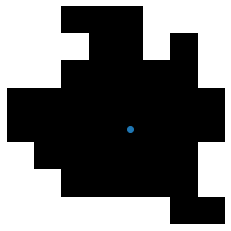
\includegraphics[width=\linewidth]{idla_40.png}
  \endminipage\hfill
  \minipage{0.32\textwidth}
    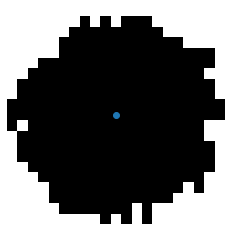
\includegraphics[width=\linewidth]{idla_300.png}
  \endminipage\hfill
  \minipage{0.32\textwidth}
    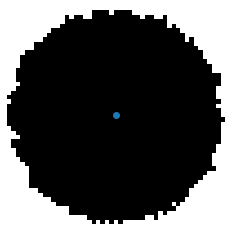
\includegraphics[width=\linewidth]{idla_1800.png}
  \endminipage
  \caption[placeholder]{IDLA clusters for n = 40, 300, and 1800. \footnotemark}
\end{figure}

\footnotetext{The code for all simulations and visualizations can be 
found in the following repository: 
\url{https://github.com/lennartCln/IDLA}}

By time $\pi r^2$ we expect the IDLA cluster to 
have the approximate shape of the ball
$ \label{D: B_r} \nonumber B_r = \{x \in \mathbb{R}^2 \,:\,  |x| < r \}$, 
where $|\cdot|$ denotes the Euclidean norm. 
The main result of this theses proves this asymptote 
and furthermore shows that fluctuations away from the ball are logarithmic. 
For real numbers $t \geq 0$ let $A(t) := A(\lceil t \rceil)$ 
and let $\mathbb{B}_r = B_r \cap \mathbb{Z}^2 \label{D: mathbb(B)_r}$.  
With these definitions we can already state the main theorem. 

\begin{theorem}[Logarithmic Fluctuations] 
  \label{log fluctuation}
  For each $\gamma \geq 1$ there is an 
  \hbox{$a = a(\gamma) < \infty$}
  and $r_0 = r_0(\gamma)$ such that 
  $$
  \mathbb{P} \big( \{ 
    \mathbb{B}_{r-a\ln r} 
      \subset A(\pi r^2) \subset \mathbb{B}_{r+a\ln r} \}
      ^c \big)
    \leq r^{-\gamma},
  $$
  for all $r > r_0$.  
\end{theorem}

Since $\sum_{r \in \mathbb{N}} r^{-\gamma}$ converges for 
$\gamma > 1$, 
Theorem \ref{log fluctuation} implies 
(using Borel-Cantelli) 
that almost surely there is just a finite number 
of $r \in \mathbb{N}$ such that 
$\mathbb{B}_{r - a \ln r} \not\subset A(\pi r^2)$ 
or $A(\pi r^2) \not\subset \mathbb{B}_{r+ a \ln r}$. 

For the proof of Theorem \ref{log fluctuation},  
I will follow Jerison, Levine, and Sheffield \cite{jerison} 
and fill out the steps omitted in the paper.


\subsection{A Brief History of IDLA Shape Results}
The model was first proposed in chemical physics by 
Meakin and Deutch \cite{meakinDeutsch} who already 
questioned the smoothness of the boundary of the cluster. 
Lawler, Bramson, and Griffeath \cite{lawler92} were 
the first who identified the asymptotic shape (in every dimension)
as the trace of Euclidean balls.
More precisely, they proved that for $\epsilon > 0$ it is 
\hbox{$\mathbb{B}_{r - \epsilon r} 
\subset A(\pi r^2)
\subset \mathbb{B}_{r+\epsilon r}$}, 
almost surely
for $r$ sufficiently large. 
Later, this result was better quantified by Lawler \cite{lawler95}, 
showing that the fluctuation from circularity is 
(up to logarithmic factors) at most  
$O(r^{1/3})$. 
The latter result had not been 
improved until  
Asselah-Gaudillière \cite{gaudilliere} 
and 
Jerison-Levine-Sheffield \cite{jerison} independently obtained 
that the fluctuation is bounded by $O(\log r)$.
Even though simulations \cite{levineSimulations}
indicate that the fluctuation is of logarithmic order, 
proving that they are of no smaller order 
is still an open problem. The best lower bound on
the fluctuation for IDLA so far is $O(\sqrt{ \log r})$, see \cite{asselah2011lower}.

IDLA has been used to understand 
anodic polishing \cite{meakinDeutsch}; 
two dimensional IDLA has been studied  
as a model for viscous fluid displacement in 
porous media \cite{PatersonFluids,ChaoTangFluids} 
and for the diffusion of oil and water particles 
\cite{CandelleroWater}.

This thesis is restricted to the two dimensional case.
When the dimension $d$ is larger than or 
equal to three, Jerison-Levin-Sheffield \cite{jerison} and 
Asselah-Gaudillière \cite{gaudilliereSublog} 
showed even smaller fluctuations, namely 
\hbox{$\mathbb{B}_{r-C \sqrt{\log r}} 
\subset A(\omega_d r^d) \subset 
\mathbb{B}_{r+\sqrt{\log^2 r}}$}, where 
$\omega_d$ is the volume of
the $d$-dimensional Euclidean ball of radius $1$.
Recent work analysed the shape of more complex cases than 
clusters based on the simple random walk on 
$\mathbb{Z}^d$, such as IDLA on the cylinder lattice \cite{JLScylinders}, 
comb lattices \cite{HussChomb}, and
supercritical percolation clusters \cite{percolationClusters}.


\subsection{Early and Late Points}

We reformulate Theorem \ref{log fluctuation} 
in terms of early and late points. 
We would expect a lattice point 
$z$ to join the IDLA cluster at time 
$\pi |z|^2$. With that in mind, we call $z$ to be
$m$-early if $z$ joins the cluster at the time 
where we would expect the shape of the cluster 
being $\mathbb{B}_{|z|-m}$; more precisely, 
$z \in \mathbb{Z}^2$ is \hbox{\textbf{$m$-early}} if 
$z \in A(\pi(|z|-m)^2)$. 
Let 
$E^m_z = \{z \in A(\pi(|z|-m)^2)\} 
\label{D: z is m early}$ denote the event
that $z$ is $m$-early, then let
\begin{equation}\label{D: def E_m(T)}
  \nonumber
  \mathcal{E}^m(T) = 
    \bigcup_{z \in A(T)} E^m_z
\end{equation}
be the event that up to time $T$ 
there was an $m$-early point in the cluster. 

Similarly, we call $z \in \mathbb{Z}^2$ to be 
\textbf{$l$-late} if 
\hbox{$z \notin A(\pi (|z| + l)^2)$.} 
By $L^l_z \label{D: z is l late}$
denote the event of $z$ being $l$-late. Let 
\begin{equation}\label{D: L_l(T)}
  \mathcal{L}^l(T) = 
    \bigcup_{z \in \mathbb{B}_{\sqrt{T/\pi} -l}} 
      L^l_z
\end{equation}
be the event that there was an $l$-late point up to time $T$. 

To divide the problem of bounding the fluctuation into the 
problems of bounding the event of single early/late 
points, we state  

\begin{lemma}[No log-early/late point implies logarithmic fluctuation]
  \label{L: logarithmic fluctuation in terms of late and early points}
  For Theorem \ref{log fluctuation} 
  it is sufficient to show that 
  for each $\gamma$ there is an $a= a(\gamma)$ 
  such that for all $r$ sufficiently large there are 
  $l$, $m < a \ln r$ such that
  \begin{equation}\nonumber
    \mathbb{P} \big( \mathcal{L}^l(T)\big) 
    +\mathbb{P} \big( \mathcal{E}^m(T)\big)
    \leq r^{-\gamma}.
  \end{equation}
\end{lemma}

\begin{remark}
  Late points quantify the inner error,
  $r - \inf \{|z| : z \notin A(\pi r^2) \}$,
  i.e., the largest deviation of $A(\pi r^2)$ 
  from  $B_r$ to the inside, and early points target the outer error,
  $\sup \{|z| : z \in A(\pi r^2) \} - r$. 
  Note that $\mathcal{L}^l(T)$ and $\mathcal{E}^m(T)$ 
  are monotonically decreasing in $l$ and $m$ 
  (since $L^l_z \supset L^{l+1}_z$, $E^m_z \supset E^{m+1}_z$). 
\end{remark}

\begin{figure}[H]
  \centering
  \captionsetup{width=.9\linewidth}
  \begin{subfigure} {0.85 \textwidth}
      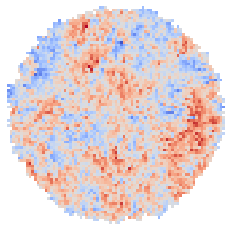
\includegraphics[width=\linewidth]{idla_5001.png}
  \end{subfigure}
      \\
    \begin{subfigure}{0.7\textwidth}
        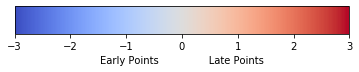
\includegraphics[width=\linewidth]{scale.png}
    \end{subfigure}
  \caption{Early (blue) and late (red) 
        points of a sample of an IDLA cluster at time $5000$. 
        Points $z \in \mathbb{Z}^2$ joining the IDLA cluster 
        at time about $\pi |z|^2$ are colored in gray.
        No point is earlier than $3$-early 
        or later than $3$-late.
        See Figure \ref{F: histo IDLA 5000} in Section \ref{sec: high level proof of log fluct}
        for a histogram of early and late points.}
  \label{F: IDLA 5000}
\end{figure}

\begin{proof}
  [Proof of Lemma \ref{L: logarithmic fluctuation in terms of late and early points}]
  It is 
  \begin{equation}\label{eq: early points as a union}
  \begin{split}
    \mathcal{E}^m(T) &= 
      \bigcup_{z \in A(T)} 
        \big{\{}z \in A(\pi(|z|-m)^2)\big{\}}\\
    &= \bigcup_{z \in A(T)} 
        \;\; \bigcup_{n \leq \pi(|z|-m)^2} 
          \{z \in A(n)\}\\
    &= \bigcup_{n \leq T} 
        \Big{\{}\text{there is a} 
          \;z : z \in A(n) \;\;
            \text{and}\;\; 
            z \notin \mathbb{B}_{\sqrt{n/ \pi}+m} 
            \Big{\}}\\
    &= \bigcup_{n \leq T} 
        \Big{\{} \mathbb{B}_{\sqrt{n/ \pi}+m} 
          \not\supset A(n) \Big{\}},
  \end{split}
  \end{equation} 
  similarly, 
  \begin{equation}\nonumber
    \mathcal{L}^l(T) 
    = \bigcup_{n \leq T} 
      \Big{\{} \mathbb{B}_{\sqrt{n/\pi} -l} 
        \not\subset A(n) \Big{\}}.
  \end{equation} 
  Therefore, using the monotonicity of $\mathcal{L}^l(T)$ 
  and $\mathcal{E}^m(T)$ in $l$ and $m$,
  we get for $T = \pi r^2$ and 
  $l, \, m < a \ln r$,   
  \begin{equation}\nonumber
  \begin{split}
    \mathbb{P}& \big( 
      \mathbb{B}_{r - a \ln r} \not\subset A(T) 
        \;\; \text{or} \;\;  
          A(T) \not\subset \mathbb{B}_{r+a \ln r}\big)\\
    &\leq \mathbb{P} \big( \mathbb{B}_{r-l} \not\subset A(T)\big) 
        + \mathbb{P} \big( A(T) \not\subset \mathbb{B}_{r+m} \big)\\
    &\leq \mathbb{P} \big( \mathcal{L}^l(T)\big) 
    +\mathbb{P} \big( \mathcal{E}^m(T)\big).
  \end{split}
  \end{equation}
\end{proof}

\subsection{Proof Sketch}
Lemma \ref{L: logarithmic fluctuation in terms of late and early points} 
implies that in order to prove Theorem \ref{log fluctuation} 
it suffices to show that $l$-late and $m$-early points 
are unlikely for $l$ and $m$ of logarithmic order. 
Here, I will briefly sketch the proof of this statement.
For readability in text passages I often refer to probabilities of events as if 
they were boolean expressions.
\\~\\
We define the \textbf{grid} $\mathcal{G}$ by,
\begin{equation} 
  \label{D: grid}
  \mathcal{G} := \{x+iy \,|\,
    x \in \mathbb{Z} \; \text{or} \;  y \in \mathbb{Z}\} \subset \mathbb{C}.
\end{equation}
On the grid we define in Section \ref{sec: grid BM} a continuous process 
which we call grid Brownian motion and for integer times behaves 
like a random walk on $\mathbb{Z}^2$ (as a subset of $\mathcal{G}$); 
for intermediate times it behaves like a one 
dimensional Brownian motion on the edges of $\mathcal{G}$. 
Furthermore, we will give a definition of harmonicity on the grid 
(see Section \ref{sec: grid-harmonic functions}) and prove 
that a function of grid Brownian motion is also a martingale if 
the function is grid harmonic (see Theorem \ref{harmonic function of grid BM}).  
This result for grid-harmonic functions is analogous to  
the fact that harmonic functions applied to Brownian motions are martingales.
For $\zeta \in \mathbb{Z}^2$ we will define  
a function $H^{\zeta}$ on the grid, see \eqref{D: H zeta}, which 
is grid harmonic and approximates the discrete Poisson kernel for the ball $\mathbb{B}_{|\zeta|}$. 
Moreover is $H^{\zeta}$ close to the continuum Poisson kernel for 
the ball $B_{|\zeta|}$ (Lemma \ref{L: H close to F}). 
We will derive some properties of $H^{\zeta}$ 
such as an approximate mean-value property (see Lemma \ref{Properties of H} (f)) 
from the continuum Poisson kernel. 

We will define the grid IDLA (see Section \ref{sec: grid idla}), 
whose underlying particles are grid Brownian motions with similar 
stopping rules as the particles (random walks) of the IDLA. Hence, for integer times 
the grid IDLA behaves like the IDLA.  

Our main tool is the process $M^{\zeta}$, which is defined by the values of 
$H^{\zeta}$ on the particles of the grid IDLA 
(see Section \ref{sec: define the martingale}). 
Since $H^{\zeta}$ is grid harmonic and since the underlying particles 
of the grid IDLA are grid Brownian motions (and therefore continuous), 
we can conclude that $M^{\zeta}$ is a continuous martingale (see Lemma \ref{lemma M : martingale}). 
Hence, we can represent $M^{\zeta}$ by a time-changed Brownian 
motion (using Theorem \ref{theorem DDS}). 
Applying this outcome and a bound on large deviations of 
Brownian motions (Lemma \ref{Exponential Inequality}), we can conclude that 
the deviation of $M^{\zeta}$ is unlikely to be large while
its quadratic variation is small (Lemma \ref{Small QV implies small martingale}).
Analyzing the behavior of $M^{\zeta}$ and its 
quadratic variation on the event of early and late points 
near $\zeta$ will be the next aim. 

If we choose $\zeta$ outside the ball $\mathbb{B}_r$ 
(from which we want to measure the fluctuations of \hbox{$A(T)$}, for $T = \pi r^2$),
then $M^{\zeta}$ is large on the event of an early point near $\zeta$ and no late point 
(see \eqref{eq: bound M on Q}).
For this implication, we use that close to an early point there are many points part of the IDLA cluster 
(see Section \ref{sec: no thin tentacles}) and that $H^{\zeta}$ is large near $\zeta$ (Lemma \ref{Properties of H}).
In addition, on the same event the quadratic variation is small (see \eqref{eq: bound QV on Q}). 
According to Lemma \ref{Small QV implies small martingale}, however, 
the quadratic variation is large if the martingale is large, i.e., 
the event —an early point but and no late point— is unlikely to occur; 
in other words: early points imply late points (see Lemma \ref{Early Points Imply Late Points}). 

Under assistance of the same tools we will prove that late points imply early points 
(Lemma \ref{Late Points Imply Early Points}). 
If we choose $\zeta$ inside $\mathbb{B}_r$ and $\zeta$ is a late point, 
then no particle reaches $\zeta$. 
Hence, and by the mean-value property of $H^{\zeta}$,  
the martingale $M^{\zeta}$ is small (large deviation). 
If in addition there is no early point, then  
its quadratic variation is large (Lemma \ref{No early point then small QV 2}). 
Again, the result—late points imply early points—follows since 
by Lemma \ref{Small QV implies small martingale} the deviation of the martingale $M^{\zeta}$ 
cannot be large while its quadratic variation is small.

Lemma \ref{Early Points Imply Late Points} and \ref{Late Points Imply Early Points} 
are the key ingredients for the final step 
of the proof of the main result (provided by Section \ref{Sec: Proof Lof Fluctuation}), 
iterating alternatingly the contraposition of Lemma \ref{Early Points Imply Late Points} 
(i.e., no late point implies no early point)
and Lemma \ref{Late Points Imply Early Points}
(i.e., no early point implies no late point).
We will recursively define sequences $l_i$ and $m_i$ starting 
with $l_0$ being of order $\sqrt{T}$.
Then Lemma \ref{No Very Late Point} (an a priori bound on the event of 
the absence of $\sqrt{T}$-late points) implies
that there is no $l_0$-late point by time $T$.  
Choosing $m_0$ to be $l_0$ up to a multiplicative constant, 
Lemma \ref{Early Points Imply Late Points} 
(no $l_0$-late points imply no $m_0$-early points) gives us  
the absence of $m_0$-early points by time $T$.  
Similarly, we can conclude from Lemma \ref{Late Points Imply Early Points} 
(no $m_0$-early point implies no $l_1$-late point) that there is no 
$l_1$-late points by time $T$ if we choose $l_1$ to be approximately $\sqrt{m_0}$.
By this choice $l_1$ is smaller than $l_0$, i.e., even less late points are unlikely. 
Hence, if we keep on assigning $l_i$ and $m_i$ according to these rules 
(see also \eqref{eq: def of l_i, m_i}), 
we obtain decreasing sequences for which there are no $l_i$-late and $m_i$-early points.
The assumptions of Lemma \ref{Early Points Imply Late Points} or \ref{Late Points Imply Early Points} 
are fulfilled for $m_i$ or $l_i$ being larger than $\ln T$. 
Therefore, we stop the iteration when reaching this threshold 
and we end up with $l$ and $m$ being of order $\ln T$.
According to Lemma \ref{L: logarithmic fluctuation in terms of late and early points} 
this is what we needed to show.


\section{Preliminaries}

\subsection{Brownian Motions}
Let $\mathcal{B}(t)$, $t \geq 0$ be a standard Brownian motion
starting in the origin, and by
$\tau_{(a,b)} = \inf\{s \geq 0 \,|\,\mathcal{B}(s) \notin (a,b)\}$ 
denote its exit time from the interval $(a,b)$.
Lemma \ref{exit times of BM} provides 
an upper bound for this exit time and 
\hbox{Lemma \ref{Exponential Inequality}} bounds large deviations of $\mathcal{B}$. 
In Section \ref{sec: Martingales} and \ref{sec: Proof QV Bounds} 
we will use these lemmas to bound martingales, 
which will be represented by Brownian motions. 


\begin{lemma}[Exit times of Brownian motions]
  \label{exit times of BM}
  Let $0 < d \leq c$ and $\lambda > 0$ with
  \hbox{$\sqrt{\lambda}(c+d) \leq \frac{3}{\sqrt{2}}$}, 
  then
  $$
  \Ex \big( e^{\lambda \tau_{(-d,c)}} \big)
  \leq 1 + 20 \lambda c d.
  $$
\end{lemma}

\begin{proof}
  The first part of the proof follows the idea 
  of \cite{revuz}, Ch. II, Prop. 3.7. The estimations
  of the second part follow Lemma 5 in \cite{jerison}.

  Obtain that for a standard Brownian motion $\mathcal{B}(t)$
  started in $0$,
  \begin{equation}\nonumber
  M^s(t) :=
    \exp 
      \Big( i s \Big(
      \mathcal{B}(t) - \frac{c-d}{2} \Big) + 
      \frac{s^2}{2}t \Big)
  \end{equation}
  is a (complex) martingale. Hence, the same holds true for 
  \begin{equation}\nonumber
    N^s(t) := 
    \frac{1}{2} \big( M^s(t) + M^{-s}(t) \Big) 
    = \exp ( t \,s^2 /2 ) 
        \cdot \cos \Big(
        s \Big( \mathcal{B}(t) - \frac{c-d}{2}\Big) \Big).
  \end{equation} 
  Since $N^s(t \land \tau_{(-d,c)})$ is bounded by 
  $\exp ( c s^2 /2)$, it is uniformly integrable.  
  Therefore, if $s \in [0, \pi (c+d)^{-1})$, 
  it is by optional sampling theorem (\cite{revuz}, Ch. II, Cor. 3.6), 
  \begin{equation}\nonumber
  \begin{split}
    \Ex &\big( \exp 
      \big( \tau_{(-d,c)} \, s^2 / 2 \big) \big)\\
      & =  \Ex \Big(
      \exp \big(  \tau_{(-d,c)}\, s^2 /2 \big)
        \cdot \cos \Big(
        s \Big( \mathcal{B}(\tau_{(-d,c)}) - 
        \frac{c-d}{2} \Big) \Big) \Big)
        \cdot \Big( \cos  s \frac{c+d}{2} \Big)^{-1} \\
    & = \Ex \big( N^s(\tau_{(-d,c)}) \big) 
          \cdot \Big( \cos
          s \frac{c+d}{2} \Big)^{-1}\\
    & =  \Ex \big( N^s(0) \big) 
          \cdot \Big( \cos s \frac{c+d}{2} \Big)^{-1}\\
    & = \Big(\cos s \frac{c-d}{2} \Big) 
          \cdot \Big(\cos s \frac{c+d}{2} \Big)^{-1}\\
    & = \cos(s a) 
        \cdot \cos (s b)^{-1},
  \end{split}
  \end{equation}
  where in the last equation we defined  
  $a = \frac{c-d}{2}$, $b = \frac{c+d}{2}$.

  Cosine is decreasing and concave on $[0,\frac{\pi}{2}]$; as a result, we have
  $$
  \cos y - \cos x \geq (y-x) \cos 'y,
  $$
  for $0 \leq x \leq y \leq \frac{\pi}{2}$.
  Hence, for $0 \leq s a \leq s b \leq \frac{\pi}{2}$ the estimation
  $$
  \cos(s a) \leq
    \cos(s b) + s(b-a) 
      \sin(s b)
  $$ 
  provides 
  $$
  \cos(s a) 
        \cdot \cos (s b)^{-1}
  \leq 1 + s(b-a) \tan (s b).
  $$
  Thus, using $\tan x < 10x$, for $0 < x \leq \frac{3}{2}$, 
  \begin{equation}
    \begin{split}
      \cos(s a) 
            \cdot \cos (s b)^{-1}
      & \leq 1 + 10 s^2 b(b-a) \\
      & \leq 1 + 10 s^2 (b-a)(b+a)\\
      & = 1 + 20 \lambda c d, \nonumber
    \end{split}
  \end{equation}
  for $0 \leq \sqrt{\lambda} (c-d) 
  \leq \sqrt{\lambda}(c+d) 
  \leq \frac{3}{\sqrt{2}}$. 
\end{proof} 

\begin{lemma}[Exponential inequality]
  \label{Exponential Inequality}
  For $a \geq 0$, it is
  $$
  \mathbb{P} \bigg( \sup_{s \in [0,t]} 
      \mathcal{B}(s) \geq at \bigg)
        \leq e^{-a^2 t / 2}.
  $$
\end{lemma}

The proof is an application of Doob's $L^1$-inequality 
(\cite{revuz}, Ch. II, Theorem 1.7)
to the martingale $M^{\alpha}(t) = 
\exp \big(\alpha \mathcal{B}(t) - \frac{\alpha^2}{2}t \big)$. 
The detailed proof can be found in \cite{revuz}, Ch. II, Prop. 1.8.


\subsection{Martingales} 
\label{sec: Martingales}
In this section, we collect some properties of martingales 
useful for this thesis.\\~\\
In what follows, we let $X(t)$, $t\geq 0$ be a real-valued process;
$(\Omega, \mathcal{F}, \mathbb{P})$ a probability space 
and $\mathcal{F}_t$ a filtration of $\mathcal{F}$. 

If $X(t)$ is adapted to $\mathcal{F}_t$ and 
\begin{itemize}
  \item $\Ex (|X(t)|) < \infty$ for every $t \geq 0$ and 
  \item $\Ex( X(t) \,|\, \mathcal{F}_s) = X(s)$ a.s. for all $0\leq s < t$,
\end{itemize}
then $X$ is a \textbf{martingale} (w.r.t. $\mathcal{F}_t$).
In order to define the quadratic variation of $X$, 
let $\Delta$ be a subdivision of the interval 
$[0,t]$ with $0 = t_0 < t_1 < ... < t_n = t$ 
and denote the modulus of $\Delta$ by 
$|\Delta| = \sup_i | t_{i} - t_{i-1} | \label{D: modulus of subdicison}$. 
We set 
\begin{equation}\nonumber
  T^{\Delta}_t = \sum_{i=1}^n \big( X(t_{i+1}) - X(t_i) \big)^2.
\end{equation} 
We say $X$ is of finite quadratic variation if there exists 
a process $\langle X,X \rangle$ such that for every sequence 
$\Delta_i$ of subdivisions of $[0,t]$ with 
$|\Delta_i| \rightarrow 0$ as $i \rightarrow \infty$, 
\begin{equation}\label{D: QV}
  \nonumber
  \lim_{i \rightarrow \infty} 
    \mathbb{P} (|T^{\Delta_i}_t - \langle X,X \rangle_t| > \epsilon) = 0,
\end{equation}
for every $\epsilon > 0$. 
The process $\langle X,X \rangle_t$ (sometimes $\langle X \rangle_t$) 
is called the \textbf{quadratic variation} (QV) of $X$. 

The following lemma enables us to represent any martingale 
with divergent quadratic variation as a time-changed Brownian motion. 

\begin{theorem}[Dambis Dubins-Schwarz]
  \label{theorem DDS}
  Let $M(\mydot)$ be an a.s. continuous $\mathcal{F}_t$-martingale,
  which vanishes at time $0$ and with 
  $\langle M \rangle _{\infty}  = \infty$. Set 
  \begin{equation}
    T_t = \inf \{ s \geq 0 \,|\, 
      \langle M \rangle _s > t \}. 
      \nonumber
  \end{equation}
  Then $\mathcal{B}(t) := M(T_t)$ 
  is a Brownian motion adapted to $\mathcal{F}_t$ and, vice versa,  
  $M(\mydot)$ can be represented as   
  \begin{equation}\nonumber
    M(t) = \mathcal{B}( \langle M \rangle_t).
  \end{equation}
\end{theorem}

\begin{proof}
  \renewcommand{\qedsymbol}{}
  I will only sketch the two key arguments of the 
  proof. For the complete proof I refer to 
  \cite{revuz}, Ch. V, Theorem 1.6.

  For the time change $T_t$, $t\geq 0$ and the martingale 
  $M$ the assumptions for \cite{revuz}, Ch. V, Prop. 1.5 
  are fulfilled. It states that the quadratic variation 
  of the time-changed process $M_{T_{\bullet}}$ 
  equals the time-changed quadratic variation process of $M$. Hence, 
  \begin{equation}\nonumber
    \langle \mathcal{B} \rangle _t 
    = \langle M_{T_{\bullet}} \rangle _t 
    = \langle M \rangle _{T_t}
    = t.
  \end{equation} 
  Then, by Lévy's characterization theorem (\cite{revuz}, Ch. IV, Theorem 3.6) 
  $\mathcal{B}$ is a $\mathcal{F}_{T_t}$-Brownian motion.
\end{proof}

Combining Theorem \ref{theorem DDS} with Lemma \ref{Exponential Inequality} 
leads to the following large deviation bound for martingales. 

\begin{lemma} [Small QV implies small martingale]
  \label{Small QV implies small martingale}
  Let $M(t)$, $t \geq 0$ be a continuous martingale, 
  which fulfills the assumptions of Theorem \ref{theorem DDS}. 
  Then, 
  $$
  \mathbb{P} \big( M(t) \geq l, \; 
    \langle M \rangle _t \leq k \big)
      \leq  e^{-l^2/(2k)}
  $$
  and
  $$
  \mathbb{P} \big( M(t) \leq -l, \; 
    \langle M \rangle _t \leq k \big)
      \leq  e^{-l^2/(2k)},
  $$
  for all $0 < l, \, k$.
\end{lemma}

In words, if the QV of a martingale 
remains small, then a large deviation of the martingale itself is unlikely.
Or at the level of the time-changed BM $\mathcal{B}$:
if the time $\langle M  \rangle_t$ elapses slow, then it is unlikely that 
$\mathcal{B}({\langle M \rangle_t})$ is large.

\begin{proof}  
  By Theorem \ref{theorem DDS} there 
  is a Brownian motion $\mathcal{B}(t)$ such that 
  $M(t) = \mathcal{B}(\langle M  \rangle_t)$.
  Hence,
  \begin{equation}\nonumber
    \begin{split}
  \mathbb{P}( M(t) \geq l, \; 
    \langle M \rangle _t \leq k) 
  & = \mathbb{P}( 
    \mathcal{B}(\langle M  \rangle_t)
      \geq l, \; 
        \langle M \rangle _t \leq k) \\
  & \leq \mathbb{P} \bigg(
    \sup _{s \in [0,k]} 
      \mathcal{B}(s) \geq l \bigg)\\
  & \leq  e^{- l^2/(2k)}. 
  \end{split}
  \end{equation}
  The second inequality of the lemma 
  follows from the first  
  with the observation 
  $\langle -M \rangle _t = \langle M \rangle _t$.
\end{proof}


\subsection{Discrete Potential Theory} 
\label{sec: discrete potential theory}
In this section, we will define the potential kernel, 
which will be used in 
Section \ref{sec: define H} (approximating discrete Poisson kernel) 
to define a specific harmonic function. 
In Lemma \ref{L: properties of a}, we give a 
general estimate for the potential kernel and 
compute some specific values. \\~\\
Consider $\mathbb{Z}^2$ as a subset of $\mathbb{C}$ 
and denote $V = \{1, -1, i, -i\} \label{D: V}$. 
The two dimensional \textbf{simple random walk} $S(n)$
starting in $0$ can be defined
as a Markov chain with state space $\mathbb{Z}^2$, 
start $S(0) = 0$, and transition probabilities 
\begin{equation}
  \label{D: random walk}
  \nonumber
  \mathbb{P}\big( S(n+1) = z \, \big| \, S(n) = y \big) = \frac{1}{4},
  \;\;\;\text{for}\;\; z-y \in V.
\end{equation}  
For $A \subset \mathbb{Z}^2$ let 
$$
\partial_o A = \{z \in \mathbb{Z} ^2 \setminus A \, | \,
 z - y \in V,  \;\; \text{for some } y \in A  \}
$$
denote the \textbf{outer boundary} of $A$ 
and $\bar{A} := A \cup \partial_o A$ the 
\textbf{discrete closure} of $A$.
For a function $g: \bar{A} \rightarrow \mathbb{R}$ 
denote the \textbf{discrete Laplacian} $\Delta$ by 
\begin{equation}
  \label{D: discrete Lapacian}
  \nonumber
  \Delta g (z) = 
  \sum_{v \in V} \frac{1}{4} g(z + v) - g(z),
\end{equation} 
for $z \in A$. 
The function $g : \bar{A} \rightarrow \mathbb{R}$
is called \textbf{harmonic} in $A$
(with respect to the simple random walk) if 
\begin{equation}\label{D: discrete harmonic}
  \Delta g (z) = 0,
\end{equation}
for all $z \in A$.

\begin{remark}
  For such a function $g$ and a random walk $S(n)$  
  the process \hbox{$Y(n)=$} \hbox{$g((n \land \tau_A))$}
  is a martingale (by a direct calculation; see for instance \cite{lawler} Prop 6.1.1), 
  where \mbox{$\tau_A$} denotes the exit time of $S(n)$ from $A$.
\end{remark}

Define the \textbf{potential kernel} 
$a: \mathbb{Z}^2 \rightarrow \mathbb{R}_{\geq 0}$ 
by 
\begin{equation}\label{D: a}
a(z) = \sum_{n=0}^{\infty} 
   \big( \mathbb{P}(S(n) = 0) - \mathbb{P}(S(n) = z) \big). 
\end{equation}

\begin{remark}
  The convergence of $a(z)$ clearly holds  
  in the transient case; in two dimensions 
  \cite{spitzer}, Ch. 12, Prop. 1 proves the convergence.

  Moreover, \hbox{$2a(x - y)$} is equal to the expected number 
  of visits of $x \in \mathbb{Z}^2$ by a random 
  walk started in $x$ before hitting 
  $y \in \mathbb{Z}^2$, which we can obtain from 
  \cite{lawler} Proposition 4.6.3 and the translation invariance of the random walk. 
\end{remark}

\begin{lemma}[Properties of $a$]
  \label{L: properties of a}
  The potential kernel $a(\mydot)$ 
  \begin{itemize}
    \item[(a)] is harmonic everywhere except $0$, 
      \begin{equation} \nonumber
        \Delta a (z) 
        = \delta_0(z) =
        \begin{cases}
          1,\; z = 0\\
          0,\; z \neq 0,
        \end{cases} 
      \end{equation}

    \item[(b)] can be precisely estimated by
      \begin{equation}\nonumber
        a(z) = \frac{2}{\pi} \ln |z| + \lambda + O(|z|^{-2}), 
      \end{equation} 
      for a constant $\lambda > 0$,

    \item[(c)] is invariant under the dihedral symmetries, 
      i.e., for all $z \in \mathbb{Z}^2$,  
      \begin{equation}
      \nonumber
      a(z) = a(-i\bar{z}) = 
      a(i z) =a(\bar{z}) =a(-\bar{z})
      =a(-i z)=a(i \bar{z})=a(-z).
      \end{equation}

    \item[(d)] 
        $a(0) = 0, \;\;\; a(1) = 1, \;\;\text{and} \;\;\; a(1+i) = \frac{4}{\pi}.$

    \item[(e)] is subadditive, i.e., for all $x, y \in \mathbb{Z}^2$ it is
      \begin{equation}\nonumber
        a(x+y) \leq a(x) + a(y).
      \end{equation}  
  \end{itemize}
\end{lemma}
 
\begin{proof}
  \begin{itemize}
    \item[(a)] 
    Using the notation 
    $p^n(z) := \mathbb{P}(S(n) = z)$,
    we have
    \begin{equation}\nonumber
      \Delta ( p^n(0) - p^n(z) ) = p^n(z) - p^{n+1} (z),
    \end{equation} 
    for all $z \in \mathbb{Z}^2$.
    Hence, 
    \begin{equation}\nonumber
      \begin{split}
        \Delta a(z) &= 
          \lim_{n \rightarrow \infty} \sum_{i=1}^n 
          \Delta \big(p^i(0) - p^i(z) \big)\\
          & = \lim_{n \rightarrow \infty} \sum_{i=1}^n 
            \Delta \big(p^i(z) - p^{i+1}(z) \big)\\
          & = \lim_{n \rightarrow \infty} p^0(z) - p^{n+1}(z) \\
          & = p^0(z) = \delta_0.
      \end{split}
    \end{equation}

    \item[(b)] 
    This statement was first proven by Stöhr \cite{Stoer} 
    (for a more comprehensible proof see \cite{kozma}). 
    Both use the following explicit integral representation of $a(\mydot)$, 
    which appears as Prop. 4.4.3 in \cite{lawler}, 
    \begin{equation}\label{eq:rep_of_a}
      a(x) = (2\pi)^{-2} 
       \int_{[-\pi, \pi]^2}
       \frac{1-\cos x \cdot \theta}
       {1-\phi(\theta)} d \theta,
    \end{equation}
    where $\phi(\theta) = (\cos \theta_1 + \cos \theta_2)/2$ 
    denotes the characteristic function of the 
    simple random walk in $\mathbb{Z}^2$. 
    This equality can be used to derive the result.  

    \item[(c)] This follows immediately from the symmetry properties of 
    \hbox{$\mathbb{P}(S(n) = z)$.}
    
    \item[(d)] By definition it is $a(0) = 0$. 
    With $z = 0$ in (a) we obtain
    \begin{equation}\nonumber
      a(1) = 1.
    \end{equation}
    The next calculation follows Chapter 15 of \cite{spitzer}. 
    By \eqref{eq:rep_of_a} and the addition formula,
    \begin{equation}\nonumber
      \begin{split}
        a(1+i) 
        &= \frac{1}{(2\pi)^2} \int_{[-\pi, \pi]^2}
          \frac{1-\cos(\theta_1 + \theta_2)}
                {1-(\cos \theta_1 + \cos \theta_2)/2}
                d \theta\\
        &=  \frac{1}{(2\pi)^2} \int_{[-\pi, \pi]^2}
        \frac{1-\cos(\theta_1 + \theta_2)}
            {1-\Big( \cos \Big( \frac{\theta_1+\theta_2}{2}\Big)  
            \cos \Big( \frac{\theta_1 - \theta_2}{2} \Big) \Big)} \,
            d \theta.
      \end{split}
    \end{equation}
    With the transformation 
    $x = (\theta_1 + \theta_2)/2$, 
    $y = (\theta_1 - \theta_2)/2$ and 
    the symmetry properties of the integrand we can conclude 
    \begin{equation}\nonumber
    \begin{split}
      a(1+i) &= 
      \frac{1}{2 \pi^2}
        \int_{\{|x|+|y| \leq \pi\} }
        \frac{1-\cos 2 x}
        {1 - \cos x \cos y } d(x,y)\\
      &= \frac{1}{4 \pi^2} 
        \int_{[-\pi, \pi]^2} 
        \frac{1-\cos 2 x}
        {1 - \cos x \cos y } d(x,y)\\
      &= \frac{2}{\pi} 
        \int_{-\pi}^{\pi} 
        \frac{1-\cos 2 x}{|\sin x|}
        d x\\
      &= \frac{1}{\pi} 
        \int_{-\pi}^{\pi}
        \frac{(\sin x)^2}{|\sin x|} d x
      = \frac{4}{\pi}.
    \end{split}
    \end{equation}

  \item[(e)] 
    Fix $y\in \mathbb{Z}^2$ and define $g(x)= a(x+y)-a(x)$.
    By (a), $g$ is harmonic everywhere except in $0$ and $-y$. 
    By maximum principle $g$ attains its maximum in $0$ or $-y$; 
    since $g(-y) = - a(y) \leq a(y) = g(0)$, it attains its maximum 
    in $0$, i.e., for all $x,y \in \mathbb{Z}^2$,
    \begin{equation*}
       a(y) = g(0) \geq g(x) = a(x+y) + a(x).
    \end{equation*}
  \end{itemize}
\end{proof}

\begin{remark}
  By Lemma \ref{L: properties of a} (c), which 
  describes the symmetries of the potential kernel,
  it suffices to compute $a(\mydot)$ for all $z \in \mathbb{Z}^2$ with 
  $0 \leq \text{Im}(z) \leq \text{Re}(z)$. 
  It is still 
  costly to compute explicit values of $a(\mydot)$. 
  McCrea-Whipple \cite{mccrea_whipple_1940} 
  were the first who computed a large number of values of $a(\mydot)$.
\end{remark}

\subsection{Potential Theory in Continuum}
The main goal of this section is to bound the 
Poisson kernel for the ball (Lemma \ref{L: F on B_zeta+14C}). 
The Poisson kernel is harmonic in the ball. 
Hence, we may apply some general statements 
about harmonic functions which we state first.  

\subsubsection{Harmonic Analysis}
For $U \subset \mathbb{R}^2$ open, 
define the \textbf{Laplacian} $\Delta$  of a $C^2$ function 
$u : U \rightarrow \mathbb{R}$ by 
\begin{equation}\nonumber
  \label{D: cont laplacian}
  \Delta u = \partial_{x_1} \partial_{x_1} u + \partial_{x_2} \partial_{x_2} u. 
\end{equation} 
We call $u$ \textbf{harmonic} if 
\begin{equation}\nonumber
  \Delta u = 0.
\end{equation}
We use $B(z,r) = z + B_r \label{D: B(z,r)}$ to denote the ball 
with radius $r$ and center in $z \in \mathbb{R}^2$.
 

\begin{theorem}[Mean-value formula]
  \label{T: Mean-Value Formula}
  Suppose $u \in C^2(U)$ is harmonic, then 
  \begin{equation}\nonumber
    u(z) = \frac{1}{\pi r^2} \int_{B(z, r)} u(y) dy, 
  \end{equation}
  for each $B(z, r) \subset U$.
\end{theorem}

\begin{theorem}[Maximum principle]
  \label{T: maximum principle}
  If $u \in C^2(U)$ is harmonic and continuous 
  on $\bar{U}$, then 
  \begin{equation}\nonumber
    \max_{\bar{U}} u = \max_{\partial U} u.
  \end{equation}
\end{theorem}

Proofs of these basic properties of harmonic 
functions can be found for instance in \cite{evans} Chapter 2.2.


\subsubsection{Poisson Kernel for the Ball}
The aim of this section is to introduce a 
harmonic function $F^{\zeta}$, which   
plays a large role in the definition of a discrete harmonic function 
that we introduce in Section \ref{sec: define H}. 
In Lemma \ref{Propeties of F} we state basic properties
of $F^{\zeta}$, so is $F^{\zeta}$ a shift of the Poisson kernel 
for the two dimensional Euclidean ball. 
The estimations of $F^{\zeta}$ in Lemma \ref{L: F on B_zeta+14C} 
are of more specific character.\\~\\
Define $F^{\zeta} : \mathbb{C} \setminus \{\zeta\} \rightarrow \mathbb{R}$ by 
\begin{equation}  
  \label{D: def F^zeta}
  F^{\zeta} (z) = \text{Re}\, \frac{\zeta}{|\zeta| (\zeta - z)}.
\end{equation}

\begin{lemma}[Properties of $F^{\zeta}$]
  \label{Propeties of F}
    Let $\zeta \in \mathbb{C} \setminus \{0\}$, then 
    \begin{enumerate}[label=({\alph*})]   
      \item 
        \label{p: F is shift of K}
        denote the Poisson kernel for the ball $B_{|\zeta|}$ with pole in $\zeta$ by 
        \begin{equation}\label{D: poisson kernel K}
          \nonumber
          K^{\zeta}(z) = 
          \frac{|\zeta|^2 - |z|^2}{2 |\zeta| |\zeta - z|^2}.
        \end{equation}
        We have, 
        \begin{equation} \nonumber
          F^{\zeta} (z) - \frac{1}{2|\zeta|} =  K^{\zeta}(z), 
          \;\;\;\text{for all}\;\; z \neq \zeta.
        \end{equation}  

      \item 
        \label{p: level/integral curves of F} 
        The level curves of $F^{\zeta}$ are 
        the circles tangent to $B_{|\zeta|}$ at point $\zeta$. 
        The level set $F^{\zeta}(\mydot) = 0$ is the tangent line to  
        $B_{|\zeta|}$ at point $\zeta$.
        
        The integral curves of the vector field
        $\nabla F^{\zeta}$ are circles through 
        $\zeta$ with center on the tangent line 
        to $B_{|\zeta|}$ at $\zeta$ (see Figure \ref{F: integral curves}) 
        and the line through $0$ and $\zeta$.

        For both sets of curves $\zeta$ is always excluded. 

      \item
        \label{p: F: harmonic}
        $F^{\zeta}$ is harmonic in $B_{|\zeta|}$.

      \item 
        \label{p: nambla F}
        For all $z \neq \zeta$, it is  
          \begin{equation}\nonumber
            |\nabla F^{\zeta}(z) | = \frac{1}{|z- \zeta|^2}.
          \end{equation}

      \item
        \label{p: sup F^zeta over B_r}
        For $0 < R < |\zeta|$, 
        \begin{equation}\nonumber
          \sup_{z \in B_R} F^{\zeta}(z)
          = F^{\zeta} \bigg( \frac{R}{|\zeta|}\zeta \bigg) 
          = \frac{1}{|\zeta|-R}.
        \end{equation}

      \item
        \label{p: sup of F^zeta on small circles}
        For $z \in \mathbb{C}$ and $r>0$ so that 
        $\zeta \notin \bar{B}(z,r)$, it is    
        \begin{equation}\nonumber
          \sup_{\omega \in B(z,r)} 
            F^{\zeta}(\omega) - F^{\zeta}(z) 
            \leq \frac{1}{\big( |\zeta - z| - r \big)^2}.  
        \end{equation}
    \end{enumerate}
  \end{lemma}

\begin{proof}
  \renewcommand{\qedsymbol}{}
  \begin{itemize}
    \item [\ref{p: F is shift of K}] 
      Using $\text{Re} \,z = (z + \bar{z})/2$, 
      \begin{equation}\nonumber
      \begin{split}
        F^{\zeta}(z) - \frac{1}{2|\zeta|} &= 
        \frac{1}{2|\zeta| |\zeta - z|^2}
          \Big( \zeta\, \overline{(\zeta-z)} + \bar{\zeta} (\zeta -z) \Big) -\frac{1}{2|\zeta|} \\
        & = \frac{1}{2|\zeta|}\bigg( 
          \frac{1}{|\zeta-z|^2} \Big( |\zeta|^2 + |\zeta -z|^2 -|z|^2\Big) -1 \bigg)\\
        &= K^{\zeta}(z).
      \end{split}
      \end{equation}

    \item[\ref{p: level/integral curves of F}] 
      We first show that the level sets of $K^{1}$ 
      are the circles tangent to $\partial B_1$ at $1$. 
      For $z = x+iy \neq 1$ and $R \neq -1$ it is 
      \begin{equation}\label{eq: 2K^1}
        2K^1(z) = \frac{1-x^2-y^2}{(1-x)^2 + y^2} = R
      \end{equation}
      if and only if 
      \begin{equation}\nonumber
        \Big( \frac{1}{1+R} \Big)^2 
        = \Big( x - \frac{R}{1+R} \Big)^2 +y^2,
      \end{equation}  
      i.e., $z \in \partial B(m,r)$, where 
      $m =  R/(1+R)$ and $r=1/(1+R)$.
      Then the result follows since $r+m = 1$ and $\text{Im}(m) = 0$. 

      For $R=-1$, Equation \eqref{eq: 2K^1} yields 
      to the equation of the tangent line (or degenerate circle) $x=1$. 

      With the $\phi(z) := \lambda e^{\alpha i} z$ 
      for $\alpha \in [0,2\pi]$, $\lambda \in \mathbb{R}\setminus \{0\}$
      we obtain the invariance under rotation-dilation,
      \begin{equation}\label{eq: K invariant}
        K^{\phi(1)}\big( \phi(z) \big) = K^1(z).
      \end{equation}
      Hence our statement \ref{p: level/integral curves of F} 
      holds for all $\zeta = \lambda e^{i \alpha} \neq 0$, 
      and by \ref{p: F is shift of K} it holds for $F^{\zeta}$ as well. 

      To verify that the integral curves of $\nabla F$ 
      are the circles through $\zeta$ with center on the tangent line 
      to $B_{|\zeta|}$ at $\zeta$, we show geometrically that such a circle is orthogonal to all 
      level curves.
      As illustrated in Figure \ref{F: integral and level curves} below 
      we let $\varphi : (0, 2\pi) \rightarrow \mathbb{R}^2$ be a curve so that 
      the image of the curve is such a circle. 
      Let $\varphi$ start and end at $\zeta$, i.e., $\zeta$ is not in the image of $\varphi$. 
      We let $\varphi$ be directed as in Figure \ref{F: integral and level curves} below. 
      \vspace*{-7mm}
      \begin{figure}[H]
        \captionsetup{width=.75\linewidth}
        \hspace*{1cm}
        \begin{tikzpicture}[scale= 1.3] 
          \node[rotate=30] at (0,0) {
          \begin{tikzpicture}[scale= 1.3]
            %outer, level sets
            \draw [thick, name path=Binter] (0,0) circle (2cm); 
            \draw [thick] (0.7,0) circle (1.3cm); 
            \draw [thick] (1.4,0) circle (0.6cm); 
            \draw [thick] (4,0) circle (2cm); 
            \draw [thick] (3.3,0) circle (1.3cm); 
            \draw [thick] (2.6,0) circle (0.6cm); 
            %\zeta
            \fill (2,0) circle (2pt) node {};
            \fill (0,0) circle (2pt) node[] {};
            %tangent
            \draw[thick] (2,-3.6) -- (2,2);
            \draw[thick, dashed] (-2.2,0) -- (6.4,0); 
            %integral curves
            \draw[thick, blue, name path=blueTangentSouth] (2,-1.6) circle (1.6cm); 
            %arrows
            \draw [->, thick, blue] (3.6,-1.6) -- (3.6,-1.7);
            \draw [->, thick, blue] (3.6,-1.6) -- (3.6,-1.7);
            \draw [->, thick, blue] (3.6,-1.6) -- (3.6,-1.7);
            %intersections nodes p1, p2
            \fill [name intersections={of=blueTangentSouth and Binter,name=intAB}]
              (intAB-2) circle (2pt) node[] {};
          \end{tikzpicture}
          };
          %labels
          \node at (-0.3, 1.1) {$\zeta$};
          \node at (-2.1,0) {$0$};
          \node at (-3.0, 1.8) {$\gamma$};
          \node[blue] at (2.3, -1.1) {$\varphi$};
          \node at (-0.9,-2.3) {$x_0$};
        \end{tikzpicture}
        \vspace*{-25mm}
        \caption{Shown is an integral curve $\varphi$ of $\nabla F^{\zeta}$ (blue) 
          and the level sets of $F^{\zeta}$ (black). 
          Considering the kite defined by the vertices $\zeta$, $x_0$, and the centers 
          of $\varphi$ and  $\gamma$, orthogonality of $\varphi$ and $\gamma$ 
          in $x_0$ is evident.}
        \label{F: integral and level curves}
      \end{figure}
      For each point $x_0$ in the image of $\varphi$ there is 
      a level curve $\gamma$ such that 
      $\gamma(u_0) = \varphi(s_0) = x_0$ for some $s_0$, $u_0$, 
      and because $F^{\zeta}$ is constant on the level curves, 
      it is 
      $$0 = \nabla F^{\zeta}(\gamma(u_0)) \gamma'(u_0).$$ 
      Using this and the orthogonality of $\gamma'(u_0)$ 
      and $\varphi'(s_0)$, we get that
      \begin{equation}\label{eq: there is a lambda}
        \varphi'(s) = \lambda(\varphi(s)) \nabla F^{\zeta}(\varphi(s)),
      \end{equation}
      for all $s$ in the domain of $\varphi$ and 
      some real function $\lambda$. 
      Note that $\lambda(\varphi(s)) > 0$ for all $s$ 
      and that $\lambda$ is continuous 
      (since $\nabla F^{\zeta}$ and $\phi'$ are continuous). 
      Equation \eqref{eq: there is a lambda} means 
      that $\varphi$ is an integral curve of the 
      vector field $\lambda \nabla F$. 
      The result follows if we show that the images 
      of the two integral curves $\nabla F^{\zeta}$ 
      and $\lambda \nabla F^{\zeta}$ are identical. 
      To see this, define the time change $\tau(t)$ by 
      \begin{equation}\nonumber
        \int_{s_0}^{\tau(t)} \lambda( \varphi (s)) ds 
        = t - t_0,
      \end{equation}
      and by differentiating we can derive  
      \begin{equation*}
        1 = \lambda (\varphi(\tau(t))) \tau'(t).
      \end{equation*} 
      Hence, denoting $\phi(t) := \varphi(\tau (t))$, it is 
      \begin{equation}\nonumber
        \phi'(t) 
        = \lambda(\phi(t)) \, \nabla F^{\zeta}(\phi(t)) \, \tau'(t)
        = \nabla F^{\zeta}(\phi(t)),
      \end{equation}
      and $\phi(t_0) = \varphi(\tau(t_0)) = x_0$, 
      which completes this proof. 

  \item[\ref{p: F: harmonic}] 
    $F^{\zeta}(z)$ is the real part of 
    $f^{\zeta}(z) := \zeta / (|\zeta| (\zeta -z))$. 
    Since $f^{\zeta}$ satisfies the Cauchy-Riemann equations for 
    all $z \neq \zeta$, it is analytic in $B_{|\zeta|}$.
    Then $F^{\zeta}$ is harmonic in $B_{|\zeta|}$, 
    since the real (and the imaginary) part of analytic functions 
    is harmonic.

  \item[\ref{p: nambla F}]   
    Let $f^{\zeta}$ be defined as in \ref{p: F: harmonic}.
    Denote $u(z) = F^{\zeta}(z) = \text{Re}\, f^{\zeta}$ 
    and \hbox{$v(z) := \text{Im}\, f^{\zeta}$.}
    As in \ref{p: F: harmonic}, 
    $f^{\zeta}$ satisfies the Cauchy-Riemann equations. 
    Hence using Cauchy-Riemann equations, for all $z = x+iy \neq \zeta$ it is 
    \begin{equation}\nonumber
      \begin{split}
          | \nabla F^{\zeta} (z) |^2 
        & = \big( \partial_x u(z) \big) ^2 + \big( \partial_y u(z) \big) ^2 \\
        & = \big( \partial_x u(z) \big) ^2 + \big( \partial_x v(z) \big) ^2 \\
        & = \bigg| \frac{\partial}{\partial_z} 
          \frac{\zeta}{|\zeta| (\zeta -z)} \bigg|^2 \\
        &= \bigg| \frac{\partial}{\partial_z} 
        \frac{1}{\zeta -z}\bigg|^2,
      \end{split}
    \end{equation}
    and the result follows from
    \begin{equation}\nonumber
      \frac{\partial}{\partial_z} 
        \frac{1}{\zeta -z} = \frac{1}{(\zeta - z)^2},
        \;\;\; \text{for all} \; z \neq \zeta. 
    \end{equation} 

  \item[\ref{p: sup F^zeta over B_r}] 
    By maximum principle (Theorem \ref{T: maximum principle})
    and because $F^{\zeta}$ is harmonic on $B_R$,  
    it attains its maximum on the boundary $\partial B_R$. 
    The point $z \in \partial B_R$ with minimum distance to $\zeta$  
    is $z = \frac{R}{|\zeta|} \zeta$.
    By the representation of $F^{\zeta}$ provided in
    \ref{p: F is shift of K} and since $|z|$ is constant on $\partial B_R$, 
    $F^{\zeta}$ attains its maximum on $\partial B_R$ \hbox{in $z$}.
    
  \item[\ref{p: sup of F^zeta on small circles}] 
    Since $\zeta \notin \bar{B}(z,r)$, 
    $F^{\zeta}$ attains its maximum on $\partial B(z,r)$.   
    Hence, \hbox{using \ref{p: nambla F},}
    \begin{equation}\nonumber
    \begin{split}
      \sup_{\omega \in B(z,r)}  
        F^{\zeta}(\omega) - F^{\zeta}(z)  
      &\leq \max_{\omega \in \partial B(z,r)} 
        \int_{[z,\omega]} |\nabla F^{\zeta}| \\
      &\leq \max_{\omega \in \partial B(z,r)} 
        \frac{1}{|\zeta - \omega|^2}\\
      &= \frac{1}{\big|
      \zeta - r \frac{\zeta-z}{|\zeta-z|} -z \big|^2}\\
      &= \frac{1}{\big( |\zeta - z| -r\big)^2},
    \end{split}
    \end{equation}
    where $[z, \omega]$ denotes the line segment from 
    $z$ to $\omega$. 
  \end{itemize}
\end{proof}

\begin{remark}
  Using the notation in the proof of 
  Lemma \ref{Propeties of F} \ref{p: level/integral curves of F} we 
  obtain that $r \rightarrow \infty$ as $R \rightarrow -1$. 
  Hence, using \eqref{eq: K invariant} and $K^1(z) = F^1(z) - 1/2$,
  we get the asymptotic behavior 
  $$\lim_{|z| \rightarrow \infty} F^{\zeta}(z) = 0.$$ 
\end{remark}

Figure \ref{F: F^zeta} below exemplifies the behavior of $F^{\zeta}$ 
on circles $\partial B_r$, for $r < |\zeta|$, 
which will help for later considerations. 
\begin{figure}[H]
  \captionsetup{width=.75\linewidth}
  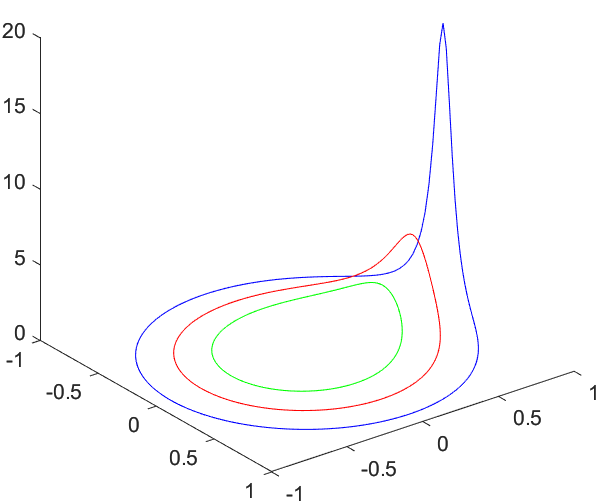
\includegraphics[width=9cm, height=6cm]{FzetaOnCircles.png}
  \centering
  \caption{The Poisson kernel $K^{1}$ on the circles 
    $\partial B_r$, for $r = 0.5$ (green), $r=0.7$ (red), and $r=0.9$ (blue).}
  \label{F: F^zeta}
\end{figure}
\vspace*{-4mm}
We now state a lemma which bounds $F^{\zeta}$ 
on circles close to $B_{|\zeta|}$. It 
will be used to show that the level sets of 
a later defined function do not 
deviate a lot from the level sets of $F^{\zeta}$.

\begin{lemma} \label{L: F on B_zeta+14C}
  For $|\zeta| > 4C>24$,
  \begin{equation}\nonumber
    \begin{split}
      &F^{\zeta}(z) - \frac{1}{2 |\zeta|} 
      \leq - \frac{C}{|z - \zeta|^2}, 
      \;\;\;\text{for}\; z \in \partial B_{|\zeta| + 14C},\\
      &F^{\zeta}(z) - \frac{1}{2 |\zeta|} 
        \geq \frac{C}{|z - \zeta|^2}, \;\;\;
        \text{for}\; z \in \partial B_{|\zeta| - 14C}.
      \end{split}
    \end{equation} 
\end{lemma}

\begin{proof}
  \renewcommand{\qedsymbol}{}
  Figure \ref{F: integral curves} sketches 
  the integral curves of 
  $\nabla F^{\zeta}$, which by Lemma \ref{Propeties of F}
  \ref{p: level/integral curves of F} are circles through 
  $\zeta$ with center on the tangent line 
  to $B_{|\zeta|}$ at $\zeta$. 
  Let $p_1$ and $p_2$ denote the points where 
  these circles are tangent to $\partial B_{|\zeta| + 2C}$, and
  let $R$ be the short segment of $\partial B_{|\zeta| + 2C}$ 
  from $p_1$ to $p_2$ (red in Figure \ref{F: integral curves} below).
  \paragraph{Step 1.} 
  Show that 
  \begin{equation}\label{eq: F on B_zeta+2C}
    F^{\zeta}(z) - \frac{1}{2 |\zeta|} 
      \leq - \frac{C}{|z - \zeta|^2}, 
      \;\;\;\text{for all} \; 
      z \in \partial B_{|\zeta| + 2C} \setminus R.
  \end{equation}
  To verify this, fix a point $z \in \partial B_{|\zeta| +2C} \setminus R$.
  By $\gamma_z = \gamma : [a,b] \rightarrow \mathbb{C}$
  denote the section of the integral curve 
  through $z$ starting at $z$ 
  and ending at some point 
  $\tilde{z} \in \partial B_{|\zeta|}$ 
  with $\tilde{z} \neq \zeta$ (as in Figure \ref{F: integral curves} below).
  \vspace*{-12mm}
  \begin{figure}[H]
    \captionsetup{width=.75\linewidth}
    \begin{tikzpicture}[scale= .8]   
      \node[rotate=30] at (0,0) {
      \begin{tikzpicture}
        %outer
        \draw [thick, name path=outerCircle] (0,0) circle (4.5cm); 
        %inner
        \draw[thick, name path=innerCircle] (0,0) circle (3cm);
        %0
        \fill (0,0) circle (2pt) node[below right] {};
        %\zeta
        \fill (3,0) circle (2pt) node[below right] {};
        %tangent
        \draw[thick, dashed] (3,-5.5) -- (3,5.5);
        %C
        \draw[thick, dashed] (-3,0) -- (-4.5,0);
        %integral curves
        \draw[thick, blue, name path=blueTangentNorth] (3,1.25) circle (1.25cm); 
        \draw[thick, blue] (3,1.9) circle (1.9cm); 
        \draw[thick, blue, name path=outerIntegralCurve] (3,2.6) circle (2.6cm); 
        \draw[thick, blue] (3,-1.9) circle (1.9cm); 
        \draw[thick, blue, name path=blueTangentSouth] (3,-1.25) circle (1.25cm); 
        \draw[thick, blue] (3,-2.6) circle (2.6cm); 
        %arrows
        \draw [->, thick, blue] (1.75,-1.3) -- (1.75,-1.2); 
        \draw [->, thick, blue] (1.1,-1.9) -- (1.1,-1.8);
        \draw [->, thick, blue] (0.4,-2.6) -- (0.4,-2.5);
        \draw [->, thick, blue] (1.75, 1.3) -- (1.75, 1.2); 
        \draw [->, thick, blue] (1.1, 1.9) -- (1.1, 1.8);
        \draw [->, thick, blue] (0.4, 2.6) -- (0.4, 2.5);
        %intersections nodes p1, p2
        \fill [ name intersections={of=blueTangentNorth and outerCircle,name=intAB}]
          (intAB-2) circle (2pt) node[below right] {};
        \fill [ name intersections={of=blueTangentSouth and outerCircle,name=intA}]
          (intA-2) circle (2pt) node[below right] {};
        \fill [ name intersections={of=outerIntegralCurve and outerCircle,name=intC}]
          (intC-1) circle (2pt) node[below right] {};
        \fill [ name intersections={of=outerIntegralCurve and innerCircle,name=intD}]
          (intD-1) circle (2pt) node[below right] {};
        % red path
        \pgfsetstrokecolor{red}
        \pgfsetlinewidth{1.1pt}
        \pgfpathmoveto{\pgfpointanchor{intAB-2}{north}}
        \pgfpatharcto{4.5cm}{4.5cm}{1}{0}{0}{\pgfpointanchor{intA-2}{north}}
        \pgfusepath{stroke}
    \end{tikzpicture}
    };
    %labels
    \node at (2.1, 1.8) {$\zeta$};
    \node at (-0.1,-0.1) {$0$};
    \node at (-4.8, -1.9) {$2C$};
    \node at (4.3, 0.6) {$p_2$};
    \node at (2.6, 3.5) {$p_1$};
    \node[red] at (3.9, 2.4) {$R$};
    \node at (-1.8, 4.6) {$z$};
    \node at (-1.9, 2.3) {$\tilde{z}$};
    \end{tikzpicture}
    \vspace*{-27mm}
    \caption{Integral curves of $F^{\zeta}$ (blue)
      connecting $\partial B_{|\zeta|}$ and 
      $\partial B_{|\zeta|+2C}$. 
       Note the difference in the length of $\gamma_z$ between 
       $z \in R$ and $z \in \partial B_{|\zeta| +2C} \setminus R$. 
       We defined $R \subset \partial B_{|\zeta| +2C}$ (red) by the arc between 
       $p_1$ and $p_2$, in which the integral curves are tangent to $\partial B_{|\zeta| +2C}$}
    \label{F: integral curves}
  \end{figure}
  Since 
  $F^{\zeta} = \frac{1}{2|\zeta|}$ 
  on
  $\partial B_{|\zeta|} \setminus \{\zeta\}$, 
  it is $F^{\zeta}(\tilde{z}) = \frac{1}{2|\zeta|}$.
  Using Lemma \ref{Propeties of F} \ref{p: F: harmonic} we see that
  \begin{equation}\nonumber
    \begin{split}
      \frac{1}{2|\zeta|} - F^{\zeta}(z) 
      &= \int_{\gamma} \nabla F^{\zeta} \\
      &= \int_{[a,b]} \nabla F^{\zeta}(\gamma(t)) \cdot \gamma '(t) dt\\
      &=  \int_{[a,b]} |\nabla F^{\zeta}(\gamma(t)) \cdot \gamma '(t)| dt \\
      & \geq \min_{y \in \gamma} \frac{1}{|\zeta - y|^2}
        \int_{[a,b]} |\gamma ' (t)| dt \\
      &= \frac{\text{Length}(\gamma)}
            {\max_{y \in \gamma} |\zeta - y|^2},
    \end{split}
  \end{equation}
  where $y \in \gamma$ means that $y$ is an
  element of the image of $\gamma$. 
  Fix some \hbox{$z \in \partial B_{|\zeta|+2C} \setminus R$}.
  Then the distance of $y$ to $\zeta$ changes just 
  a little for $y$ along $\gamma_z = \gamma$. More precisely, 
  \begin{equation}\label{eq: dist along gamma}
    \max_{y \in \gamma} |\zeta - y|^2 
    \leq 2 |\zeta - z|^2.
  \end{equation}
  This can be seen by noting that $\gamma_z$ is contained 
  in a square with vertices $z$ and $\tilde{z}$. Hence,
  \begin{equation}\nonumber
    \max_{y \in \gamma} |\zeta - y| 
    \leq |\zeta - z| + \sqrt{2|z - \tilde{z}|}.
  \end{equation}
  Since the integral curve through $p_1$ 
  is tangent to $B_{|\zeta|+2C}$ at $p_1$, we obtain 
  $|z - \tilde{z}| \leq |p_1 - \tilde{p}_1| = |p_1 - \zeta| \leq |z - \zeta|.$
  Hence, with $C>6$ we have
  \begin{equation}\nonumber
    \max_{y \in \gamma} |\zeta - y|  
      \leq |\zeta - z| + \sqrt{2|z - \zeta|}
      \leq \sqrt{2} |\zeta - z|,
  \end{equation} 
  which shows \eqref{eq: dist along gamma}. 
  By \eqref{eq: dist along gamma} and the fact that each curve connecting 
  $\partial B_{|\zeta| + 2C}$ and $\partial B_{|\zeta|}$ has 
  length at least $2C$, Equation \eqref{eq: F on B_zeta+2C} holds. 
  \paragraph{Step 2.} 
  Now we will use \eqref{eq: F on B_zeta+2C} to 
  complete the first inequality of this lemma. 
  Our strategy is to choose a circle sufficiently larger 
  than $\partial B_{|\zeta|+2C}$ so that for each point $z$ on that 
  circle the level curve $F^{\zeta}(\cdot) = F^{\zeta}(z)$ can be traced to 
  a point where the level curve intersects $\partial B_{|\zeta|+2C} \setminus R$. 
  Then apply \eqref{eq: F on B_zeta+2C} on the intersection point. 

  We choose a cone so that $R$ is inside the cone.
  Fix $\zeta$ and $C$ with $|\zeta| > 4C$. 
  Assume $\text{Im}\, \zeta = 0$. 
  We define the cone with vertex in $0$ by its 
  height $h$ (as in Figure \ref{F: h leq 2C}). 
  Also let $s$, $k$, and $\omega$ be defined as in Figure \ref{F: h leq 2C} below.
  \begin{figure}[H]
    \centering
    \captionsetup{width=.75\linewidth}
    \hspace*{0.9cm}
    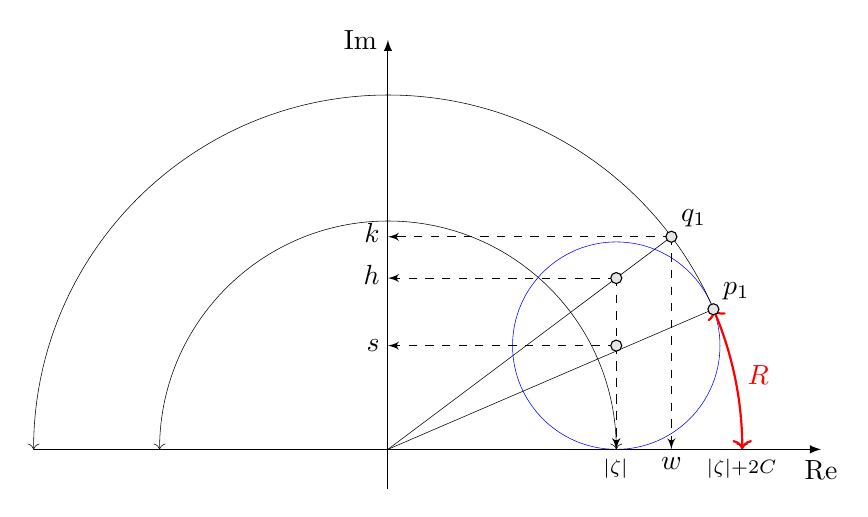
\begin{tikzpicture}[scale=1]
      \tkzInit[xmin=-4,xmax=5,ymin=-0.5,ymax=4.7]
      \tkzDrawX[noticks, label= Re]
      \tkzDrawY[noticks, label= Im]
      \tkzDefPoint(0,0){zero}
      \tkzDefPoint(2.9,0){zeta}
      \tkzDefPoint(-2.9,0){minZeta}
      \tkzDefPoint(4.5,0){zetaPlus}
      \tkzDefPoint(-4.5,0){minZetaPlus}
      \tkzDefPoint(2.9,4){zetaVerticalPlu}
      \tkzDefPoint(2.9,-4){zetaVerticalMin}
      \tkzDefPoint(6,2.725){fluchtpktPlu}
      \tkzDefPoint(6,-2.725){fluchtpktMin}
      \tkzDefPoint(4,3){rayFluPktPlu}
      \tkzInterLL(zero,rayFluPktPlu)(zeta,zetaVerticalPlu)
        \tkzGetPoint{xOne}
      \tkzInterLC(zero,rayFluPktPlu)(zero,zetaPlus)
        \tkzGetPoints{dummy}{yOne}
      \tkzInterLL(zero,fluchtpktPlu)(zeta,zetaVerticalPlu)
        \tkzGetPoint{mOne}
      \tkzDrawCircle[color=blue](mOne,zeta)
      \tkzDrawArc[color=black,<->](zero,zeta)(minZeta)
      \tkzDrawArc[color=black,<->](zero,zetaPlus)(minZetaPlus)
      \tkzInterLC(zeta,zetaVerticalPlu)(zero,zetaPlus) 
        \tkzGetPoints{A}{B}
      \tkzInterCC(zero,zetaPlus)(mOne,zeta)
        \tkzGetPoints{_}{pOne}
      \tkzDrawSegment(zero, pOne)
      \tkzDrawSegment(zero,yOne)
      \tkzDrawSegment(minZetaPlus,zetaPlus)
      %points
      \tkzPointShowCoord[ylabel=$h$](xOne) 
      \tkzPointShowCoord[xlabel=$w$,ylabel=$k$](yOne)
      \tkzPointShowCoord[ylabel=$s$](mOne)
      \tkzLabelPoint[above right](pOne) {$p_1$}
      \tkzLabelPoint[above right](yOne) {$q_1$}
      \tkzLabelCircle[above right, color=red](zero,zetaPlus)(9){$R$}
      \tkzLabelPoint[below](zetaPlus) {$_{|\zeta|+2C}$}
      \tkzLabelPoint[below](zeta) {$_{|\zeta|}$}
      %R
      \tkzDrawArc[color=red,thick,<->](zero,zetaPlus)(pOne)
      \tkzDrawPoints[size=4](mOne,pOne,xOne,yOne)
    \end{tikzpicture}
    \vspace*{-36mm}
    \caption{This figure defines $s$, $h$, $k$, $\omega \in \mathbb{R}$
      and $q_1 \in \mathbb{C}$. 
      Where $s$ denotes the radius of the integral curve  
      tangent to $B_{|\zeta| + 2C}$ (blue). We consider 
      $k$, $\omega$, and $q_1$ to be determined by $h$. 
      Otherwise, the setting is (up to rotation) the same as 
      in Figure \ref{F: integral curves}.}
    \label{F: h leq 2C}
  \end{figure}
  \vspace*{-5mm}
  The radius of the integral curve tangent to 
  $\partial B_{|\zeta|+2C}$ (blue in Figure \ref{F: h leq 2C}),  
  which is defined by $s$, is smaller than $2C$ 
  (since the center is inside the annulus $B_{|\zeta|+2C} \setminus B_{|\zeta|}$).
  Thus, we choose $h = 2C$. We will show now that 
  \begin{equation}\label{eq: tilde h and omega}
    |\zeta|+C < \omega < |\zeta| + 2C, \;\;\text{and} \;
    k \leq 3C.
  \end{equation}
  The upper bound of $\omega$ is obvious. For the lower bound, note that 
  \begin{equation}\nonumber
    \frac{\omega}{|\zeta|} = \frac{|\zeta|+2C}{\sqrt{h^2 + |\zeta|^2}}.
  \end{equation} 
  Hence, $|\zeta| + C < \omega$ holds if 
  \begin{equation}\nonumber
    \bigg( \frac{|\zeta|(|\zeta|+2C)}
        {|\zeta|+ C} \bigg)^2 -|\zeta|^2 > h^2 = 4C^2.
  \end{equation}
  The left-hand side equals 
  \begin{equation}\nonumber
    \begin{split}
      &\frac{|\zeta|^2 (2C|\zeta| + 3C^2)}{(|\zeta|+C)^2}
      = \frac{2C|\zeta|^2}{|\zeta| +C} \cdot \frac{|\zeta|+ 3C/2}{|\zeta|+C}\\
      &\geq \frac{2C|\zeta|^2}{|\zeta| +C}
      \geq \frac{2C|\zeta|^2}{|\zeta| + |\zeta|/4} 
      = \frac{8}{5} C |\zeta| 
      > 4 C^2. 
    \end{split}
  \end{equation} 
  Again we use intercept theorem and $|\zeta| \geq 4C$ to show
  \begin{equation}\nonumber
    k = h \frac{|\zeta|+2C}{|\zeta|} 
      = 2C + \frac{4C^2}{|\zeta|} 
      \leq 3C.
  \end{equation}  

  Now we will find an upper bound for the radius of the 
  circle, which runs through $q_1$ and is tangent to 
  $B_{|\zeta|}$ at $\zeta$ (see radius $r$ in Figure \ref{F: level curve over R} below).
  \vspace*{-25mm} 
  \begin{figure}[H]
    \centering
    \captionsetup{width=.75\linewidth}
    \begin{tikzpicture}[scale=0.75]
      \tkzDefPoint(0,0){zero}
      \tkzDefPoint(2.9,0){zeta}
      \tkzDefPoint(4.5,0){zetaPlus}
      \tkzDefPoint(-2.9,0){minZeta}
      \tkzDefPoint(-4.5,0){minZetaPlus}
      \tkzDefPoint(2.9,4){zetaVerticalPlu}
      \tkzDefPoint(2.9,-4){zetaVerticalMin}
      \tkzDefPoint(5,1.6){fluchtpktPlu}
      \tkzDefPoint(5,-1.6){fluchtpktMin}
      \tkzDefPoint(5,2.7){rayFluPktPlu}
      \tkzDefPoint(5,-2.7){rayFluPktMin}
      \tkzInterLL(zero,rayFluPktPlu)(zeta,zetaVerticalPlu)
        \tkzGetPoint{xOne}
      \tkzInterLL(zero,rayFluPktMin)(zeta,zetaVerticalMin)
        \tkzGetPoint{xTwo}
      \tkzInterLC(zero,rayFluPktPlu)(zero,zetaPlus)
        \tkzGetPoints{dummy}{yOne}
      \tkzInterLC(zero,rayFluPktMin)(zero,zetaPlus)
        \tkzGetPoints{dummy}{yTwo}
      \tkzInterLL(zero,fluchtpktPlu)(zeta,zetaVerticalPlu)
        \tkzGetPoint{mOne}
      \tkzInterLL(zero,fluchtpktMin)(zeta,zetaVerticalMin)
        \tkzGetPoint{mTwo}
      \tkzDrawCircle[black](zero,zeta)
      \tkzDrawCircle[black](zero,zetaPlus)
      \tkzInterLC(zetaVerticalMin,zetaVerticalPlu)(zero,zetaPlus) 
        \tkzGetPoints{A}{B}
      \tkzInterLC(zero,fluchtpktPlu)(zero,zetaPlus)
        \tkzGetPoints{dummy}{pOne}
      \tkzInterLC(zero,fluchtpktMin)(zero,zetaPlus)
        \tkzGetPoints{dummy}{pTwo}
      \tkzDrawSegment(zero,yOne)
      \tkzDrawSegment(zero,yTwo)
      %finalcircle
      \tkzDefCircle[circum](zeta,yOne,yTwo)
      \tkzGetPoint{O} \tkzGetLength{rayon}
      \tkzDrawCircle[R](O,\rayon pt)
      \tkzDrawSegment(zero,O)
      \tkzDrawSegment(minZeta, minZetaPlus)
      %R
      \tkzDrawArc[color=red,thick,<->](zero,pTwo)(pOne)
      %points
      \tkzDrawSegment[style=dashed](yOne,O) 
      \tkzDefPointBy[projection=onto zero--O](yOne)
          \tkzGetPoint{omega}
      \tkzDrawSegment(yOne,omega)
      \tkzDrawPoints[size=5](zero,zeta,pOne,pTwo,yOne,yTwo,O,omega) 
      \tkzLabelCircle[above right, color=red](zero,zetaPlus)(-10){$R$}
      \tkzLabelPoint[above=3pt](yOne) {$q_1$}
      \tkzLabelPoint[right](pTwo) {$p_2$}
      \tkzLabelPoint[above left](zeta) {$\zeta$}
      \tkzLabelPoint[above left](zero) {$0$}
      \tkzLabelPoint[below](omega){$\omega$}
      \tkzLabelSegment[left,pos=.6](yOne,omega){$k$}
      \tkzLabelSegment[above right,pos=.6](yOne,O){$r$}
      \tkzLabelSegment[above, pos=.5](minZeta,minZetaPlus){$2C$}
    \end{tikzpicture}
    \caption{$k$, $\omega$, $R$, $q_1$, and $p_2$ are as in Figure \ref{F: h leq 2C} 
      and \ref{F: integral curves} above. 
      The radius of the circle tangent to $\partial B_{|\zeta|}$ at $\zeta$ 
      and through $q_1$ is denoted by $r$. 
      This circle is a level curve of $F^{\zeta}$ 
      and contains the arc $R$, 
      where points are excluded from the inequalities \eqref{eq: F on B_zeta+2C}.}
    \label{F: level curve over R}
  \end{figure}
  \vspace*{-3mm}
  We can compute the radius $r$ using $r^2 = k^2 + (r-(\omega - |\zeta|))^2$.
  Hence with \eqref{eq: tilde h and omega}, 
  \begin{equation}\nonumber
    r = \frac{k^2 + (\omega - |\zeta|)^2)^2}{2(\omega - |\zeta|)}
      < \frac{(3C)^2 + (2C)^2}{2C} 
      < 7C.
  \end{equation}
  Since the level curves 
  partition $\mathbb{C} \setminus \{\zeta\}$, we can map  
  each point $z \in B_{|\zeta| + 2r}$ onto a 
  point $\hat{z} \in B_{|\zeta| + 2C} \setminus R$ (by following a level curve). 
  Apply \eqref{eq: F on B_zeta+2C} to $\hat{z}$ and 
  the result follows since $F^{\zeta}(z) = F^{\zeta}(\hat{z})$.

  With the same steps, one can prove the second inequality 
  of Lemma \ref{L: F on B_zeta+14C}. 
\end{proof}



\section{Stochastic Analysis on the Grid}
\label{sec: stoch analysis on the grid}
Let $\mathcal{G} \subset \mathbb{C}$ be the $\mathbb{Z}^2$-grid as defined in \eqref{D: grid}. 
Analogous to discrete functions that are harmonic 
with relation to the random walk (see \eqref{D: discrete harmonic}), 
we want to give a definition of 
a harmonic function on the grid and 
an (a.s.) continuous process on
the grid such that similar properties hold. 
We start with some topological definitions on the grid.\\~\\
The grid is equipped with the canonical topology induced by $\mathbb{C}$.
An \textbf{edge} in $\mathcal{G}$ 
is a closed line segment of length one, which connects two points of 
$\mathbb{Z}^2$ (which we consider as a subset of $\mathcal{G}$).
Denote $V = \{1,-1, i, -i\}$, 
and for $v \in V$ let $e_v \label{D: edge e_v}$ be the edge connecting $0$ and $v$. 
The \mbox{\textbf{0-cross}} $E \label{D: E}$ denotes
the interior of the union of the four edges containing $0$.
Note that $\partial E = V$ in the topology of $\mathcal{G}$.

\subsection{Grid-Harmonic Functions} 
\label{sec: grid-harmonic functions}
Using these definitions, we can 
now define harmonicity for functions which are defined on the grid.\\~\\
Let $U$ be an open subset of $\mathcal{G}$, then 
call a continuous function $f : U \rightarrow \mathbb{R}$ 
\textbf{grid-harmonic} on $U$ if
\begin{itemize}
  \item   $f$ is linear on each interval $I$, for $I$ being a 
    subset of $U \cap e$, for some edge $e$ of $\mathcal{G}$,
    and
  \item for each lattice point $z$ in $U$,
    the sum of the slopes of $f$ on the four  
      line segments starting in $z$ is zero; 
      i.e, if we denote $d_v = \partial_t \, f(z+tv)$ 
      for $v \in V$ and such $t>0$
      that $z+tv$ is part of the connected component of 
      $z$ in $U \cap (z+E)$, then we have 
      $$
      \sum_{v \in V} d_v = 0.
      $$
\end{itemize}

\begin{remark}
  If in addition
  $\partial U \subset \mathbb{Z}^2$, 
  i.e., $U$ is a union of crosses $z+E$ with 
  $z \in \mathbb{Z}^2$, 
  then for each $z \in U \cap \mathbb{Z}^2$ we can write 
  \begin{equation}\label{eq: representation of f}
    \left.f\right|_{z+E}(y) = f(z) + f_z(y-z),
  \end{equation}
  where $f_z$ is grid-harmonic in $E$ with $f_z(0) = 0$; 
  for $x \in E$ this enables us to write 
  \begin{equation}\label{eq: representation of f_z}
    f_z(x) = \sum_{v \in V} 
      \alpha_v |x| \indicator_{e_v}(x),
  \end{equation} 
  for some $\alpha_v \in \mathbb{R}$ (depending on $z$) with 
  \begin{equation}\nonumber
    \sum_{v \in V} \alpha_v = 0.
  \end{equation}

  Note, if we extend a discrete harmonic function  
  on $\mathbb{Z}^2$ continuously and 
  linearly along the edges of 
  $\mathcal{G}$, then this 
  function is grid-harmonic. 
\end{remark}

\begin{lemma}[Maximum principle]
  \label{L: maximum principle grid}
  Let $U$ be an open subset of $\mathcal{G}$. 
  For a continuous function $f: \bar{U} \rightarrow \mathbb{R}$, 
  which is grid-harmonic in $U$, we have
  \begin{equation}\nonumber
    \max_{\bar{U}} f = \max_{\partial U} f.
  \end{equation} 
\end{lemma}

\begin{proof}
  Suppose $f$ attains a strict maximum
  in $x_0 \in U \cap \mathbb{Z}^2$. 
  There is an $\epsilon > 0$ such that 
  $\bar{B}(x_0, \epsilon) \cap \mathcal{G} \subset U$. Then, 
  \begin{equation}\nonumber
    f(x_0) = \sum_{z \in \partial B(x_0, \epsilon) \cap \mathcal{G}} 
      \frac{1}{4} f(z) 
  \end{equation}
  leads to a contradiction since $f(z) < f(x_0)$. 

  Since $f$ is linear along the edges, $f$ can neither
  achieve a strict maximum on an open edge. 
\end{proof}


\subsection{Grid Brownian Motion} \label{sec: grid BM}
Construct an a.s. continuous process with state space $\mathcal{G}$, 
which acts like a Brownian motion on the edges and like a simple random 
walk on the lattice points of $\mathcal{G}$. \\~\\
Define the grid Brownian motion 
    $\beta_t : \Omega \rightarrow \mathcal{G}$
by specifying a particles movement from one lattice
point to the next. 
Let $\mathcal{B}$
be a one-dimensional standard Brownian motion and 
$$
\tau_{(-1,1)} = 
  \inf \{ t \geq 0\ \,|\, \mathcal{B}(t) \notin (-1,1) \}
$$ 
its exit time from the interval $(-1,1)$.
By $\tilde{\mathcal{B}}(t) = \mathcal{B}(t \land \tau_{(-1,1)})$ 
denote the stopped Brownian motion.
Note that $\tilde{\mathcal{B}}$
a.s. returns infinitely often to the origin before exiting $(-1,1)$. 
For $t>0$ let
\begin{equation}
  \begin{split}
    & a(t) = \sup 
      \{ s \leq t \,|\, \tilde{\mathcal{B}}(s) = 0\},\\
    & b(t) = \inf 
      \{ s \geq t \,|\, \tilde{\mathcal{B}}(s) = 0\}, \nonumber
\end{split}
\end{equation}
and call $(a(t), b(t))$ the \textbf{interval of excursion} straddling $t$, 
with the convention $\inf \emptyset = \infty$ and $\sup \emptyset = 0$.
After sampling $\tilde{\mathcal{B}}$,
choose for each interval of excursion a direction 
in $V$, uniformly and independently of one another.
The process $\varphi(t)$, $t\geq 0$  denotes the 
direction of the interval of 
excursion straddling $t$, chosen as described.
Since $\{ t \geq 0 \,|\, \tilde{\mathcal{B}}(t) = 0$ \} is a null set,
the process $\varphi(t)$ is defined almost everywhere.
By the sampled Brownian motion and the process $\varphi$,
define a process $X(t) : \Omega \rightarrow \bar{E}$,
which describes a particles movement on the $0$-cross by:
\begin{equation}
  \label{D: cross motion X}
  \nonumber
  X(t) := \varphi(t) \cdot \tilde{\mathcal{B}}(t).
\end{equation}
We call $X$ a \textbf{cross motion} on $E$.
In particular, the particle's distance to $0$ is distributed 
like $|\tilde{\mathcal{B}}(\mydot)|$.
By $\mathcal{F}^X$ denote the natural filtration of $X$.

Let $X^1,\, X^2, \, X^3,...$ be independent processes defined as above; 
for each such process let 
$\tau^i_E = \inf \{ t \geq 0 \,|\, X^i(t) \notin E\}$
be the hitting time of $\partial E$. 
Then for $t \geq 0$ define
$$ 
  T_t = \max \Big{\{} n \in \mathbb{N} 
  \,\Big|\, 
  \sum_{i=1}^n \tau^i_E \leq t
  \Big{\}},
$$
the largest number of stopping times $\tau^i_E$, 
which can elapse before time $t$. 
Furthermore, for $t\geq 0$ denote the overhanging time
$$
  t' :=  t - \sum_{i=1}^{T_t} \tau^i_E 
  \in [0,\tau^{n+1}_E).
$$
Now we define the \textbf{grid Brownian motion}
$\beta(t)$ by the sum of the lattice points adjacent to $0$ 
reached by the first $T_t$ processes
$X^1 \, ,..., \, X^{T_t}$ plus the position of the last particle,
which has not been stopped by time $t'$, i.e.,
\begin{equation}\label{eq: def of grid BM}
  \beta(t) = \sum_{i=1}^{T_t} X^i(\tau^i_E) + X^{T_t+1}(t').
\end{equation}

\begin{remark}[on grid Brownian motions]
  With 
  \begin{equation}
    \nonumber
    \gamma^0 = 0, \;\; \;\;
    \gamma^{n+1} = \inf \big{\{}
         t > \gamma^n \,\big|\,
   \beta (t) \in 
   \mathbb{Z}^2 \setminus \{\beta(\gamma^n)\}
   \big{\}},
  \end{equation}   
  the process $Y(n) = \beta(\gamma^n)$ restricted to
  $\mathbb{Z}^2$, is distributed like a simple random walk.

  It is $\{T_t = k\} \in 
  \sigma(\tau^1_E,\,...\,,\tau^{k+1}_E)$, 
  but $T_t$ is not a stopping time 
  with respect to the natural 
  filtration of $\beta$. 
\end{remark}

\begin{remark}[on cross motions]
  Since the directions $\varphi$ are chosen after sampling 
  the Brownian motion, the elementary Markov property 
  does not hold by definition for $X$. 
  As a substitute for the Markov property, we 
  can define a process 
  $\hat{X}^y(\mydot)$, for $y \in E$, such that 
  for each Borel set $A$ of $E$ and $s,u \geq 0$, it is 
  \begin{equation} \label{eq: def of hat X}
      \mathbb{P}\big(X(s+u) \in A 
      \,\big|\, \mathcal{F}^X_s \big) =
      \mathbb{P} \big( \hat{X}^{X(s)}(u) \in A 
        \,\big|\, X(s) \big).
    \end{equation}
  Roughly, $\hat{X}^y$ can be constructed by
  running a one-dimensional Brownian motion started in 
  $|y|$ and stopped on exiting $(-1,1)$. For the 
  first interval of excursion, choose the 
  direction $d(y)$, which for $y \in E$ can be defined by 
  \begin{equation}
    \label{D: direction d}
    \nonumber
    d(y) = \sum_{v \in V} v \cdot \indicator_{e_v}(y) \in V.
  \end{equation}
  For later intervals of excursion, 
  uniformly and independently choose directions from $V$.
  In case of $y = 0$, for all intervals 
  of excursion choose the direction uniformly and independently.
  As for $X$, define $\hat{X}^y(t)$ by the product of the Brownian motion 
  (started in $|y|$ stopped on exiting $(-1,1)$) at time 
  $t$ and the direction of the interval of excursion \hbox{straddling $t$.}
\end{remark}


\subsection{Harmonic Functions of Grid Brownian Motions} 
\label{sec: ham of grid BM}
The main result of this section is Theorem \ref{harmonic function of grid BM}. 
It states that applying a grid-harmonic function to a
grid Brownian motion preserves the martingale property. 
It may be considered as an analog (or combination)
of the fact that a discrete harmonic function applied 
to a random walk or a harmonic function applied to a Brownian motion is a martingale 
(the discrete case holds by definition; continuous case can be shown by Itô's formula). 
Lemma \ref{L: harmonic on cross} and \ref{L:remains to consider the first cross motion} 
are the preliminary work for the proof of Theorem \ref{harmonic function of grid BM}. 
\\~\\
In this section, for a grid BM $\beta$ and 
$A \subset \mathcal{G}$ we let 
\hbox{$\tau_A = \inf \{s \geq 0 \,|\, \beta(s) \notin A\}$}
and the left limit  
\begin{equation}\nonumber
  f \big(\beta(t \land \tau_A -) \big) = 
 \lim_{u \uparrow \tau_A} 
    f \big(\beta(t \land u) \big).
\end{equation}
By $\mathcal{F}$ denote the natural 
filtration of $\beta$.

\begin{theorem}
  \label{harmonic function of grid BM}
  Let $\beta$ be a grid Brownian motion and 
  $A$ be an open subset of $\mathcal{G}$.
  Assume that $f: A \rightarrow \mathbb{R}$ 
  is grid-harmonic on $A$. Then
  \begin{equation}\nonumber
    f \big( \beta(t \land \tau_A -) \big)  ,\; t \geq 0  
  \end{equation} 
  is a martingale with relation to 
  $\mathcal{F}_t$.
\end{theorem}

We will reduce the problem to subsets 
$A \subset \mathcal{G}$ with 
$\partial A \subset \mathbb{Z}^2$. 
For such an $A$ and $z \in A \cap \mathbb{Z}^2$, write 
\begin{equation}\nonumber
  \left.f\right|_{z+E}(x) = f(z) + f_z(x-z),
\end{equation} 
where $f_z: E \rightarrow \mathbb{R}$ is as 
in \eqref{eq: representation of f_z};
in particular grid-harmonic and $f_z(0)= 0$. 
By $\hat{f}_z: \bar{E} \rightarrow \mathbb{R}$ 
denote the function $f_z$ that is continuously extended to $\bar{E}$. 

\begin{remark}
  We have not assumed that $f: A \rightarrow \mathbb{R}$ is 
  continuously extendable to the boundary. 
  Hence, (according to Figure \ref{fig: set A}) for 
  $z_1 +1 = z_2 + i = \zeta \in \partial A$ 
  with $\zeta \in \mathbb{Z}^2$ it may be
  \begin{equation}\nonumber
    f(z_1) + \hat{f}_{z_1}(1) 
    \neq f(z_2) + \hat{f}_{z_2}(i),
  \end{equation}
  where $z_1$, $z_2 \in A$; i.e., 
  on the event $\beta(\tau_A)= \zeta$ the limit $f(\beta(\tau_A-))$ 
  depends on whether the last lattice 
  point $\beta$ passed, before hitting $\zeta$, was $z_1$ or $z_2$.
  \begin{figure}[H]
    \captionsetup{width=.9\linewidth}
    \hspace*{2cm}
    \begin{tikzpicture}[scale=2]
    \draw (-0.2, 0) -- (-2.2, 0) 
          (-1, 0.8) -- (-1, -1.2)
          (0.8, -1) -- (-1.2, -1)
          (0, -0.2) -- (0, -1.2)
          (-2, 0.2) -- (-2, -0.2);
    \draw[dotted, thick] 
      (-2.2, 0) -- (-2.6, 0) 
      (-2, 0.2) -- (-2, 0.6)
      (-2, -0.2) -- (-2, -0.6)
      (-1, -1.2) -- (-1, -1.6) 
      (0, -1.2) -- (0, -1.6)
      (-1.2, -1) -- (-1.6, -1);
    \draw[-), thick]  (0, -0.2) -- (0, -0.19);
    \draw[-), thick] (-0.2,0)-- (-0.19,0);
    \draw[-), thick] (-1, 0.8)-- (-1, 0.81);
    \draw[-), thick] (0.8,-1) -- (0.81, -1);
    \draw[fill] (0, 0) circle   [radius= 1.3pt];
    \draw[fill] (-1, 0) circle  [radius= 1.3pt];
    \draw[fill] (-1, -1) circle [radius= 1.3pt];
    \draw[fill] (0, -1) circle  [radius= 1.3pt];
    \draw[fill] (-2, 0) circle  [radius= 1.3pt];

    \draw	(0, 0)  node[anchor=south west] {$\zeta$}
          (0, -1) node[anchor=south west] {$z_2$}
          (-1, 0) node[anchor=south west] {$z_1$};
    \end{tikzpicture}
    \caption{Set $A \subset \mathcal{G}$ with 
      $\zeta \in \partial A$, $\zeta \notin A$, and 
      $\zeta \in \mathbb{Z}^2$.}
      \label{fig: set A}
  \end{figure}
  Therefore, Theorem \ref{harmonic function of grid BM}
  makes use of the left limit. 
  If we additionally assume that 
  $f$ is continuous on the whole grid $\mathcal{G}$, 
  then the theorem holds without the left limit.
  Since $H^{\zeta}: \mathcal{G} \rightarrow \mathbb{R}$ (defined in the next section) 
  is continuous on $\mathcal{G}$ (see \eqref{D: a}; the potential kernel $a(z)$ 
  converges for each $z \in \mathbb{Z}^2$) and grid-harmonic on $\OZ$, 
  we will not need to consider the left limit of $H^{\zeta}$.    
\end{remark}

To prove this theorem, we will reduce the 
problem to the martingale property 
of cross motions $X$, defined in \ref{D: cross motion X}.
In the sequel let $\mathcal{F}^X$ denote its natural filtration and let
\begin{equation}\nonumber
  \tau^X_B = \inf \{t\geq 0 \,|\, X(t) \notin B \},
  \;\;\;\text{and} \;\;
  \tau^i_B = \tau^{X^i}_B,
\end{equation}
for some cross motion $X^i$ and a subset $B$ of $E$.
The main ingredients for the proof of 
Theorem \ref{harmonic function of grid BM} are the following two lemmas. 

\begin{lemma}
  \label{L: harmonic on cross}
  Let $X$ be a cross motion; $B$ be an open subset of the $0$-cross $E$;
  and $g: B \rightarrow \mathbb{R}$ grid-harmonic on $B$, then 
  \begin{equation}\nonumber
    g(X(t \land \tau^X_B)), \; t \geq 0  
  \end{equation}
  is a martingale w.r.t. $\mathcal{F}^X$. 
\end{lemma}

We will now introduce some definitions related to the grid BM $\beta$. 
For $A$ as in Theorem \ref{harmonic function of grid BM} define 
\begin{equation}\nonumber
  \begin{split}
    & \nu^0 = 0, \\ 
    & \nu^{l+1} = \inf \big{\{} u > \nu^{l} 
              \,\big|\, 
                \beta(u \land \tau_A) 
                \in \mathbb{Z}^2 \setminus 
                \{ \beta(\nu^{l} \land 
                \tau_A)\} \big{\}}.
  \end{split}
\end{equation}
For $t\geq 0$ denote
\begin{equation}\nonumber
  N_t = \max \{ k \in \mathbb{N} \,|\, 
            \nu^k \leq t\}
\end{equation}
and $t^l = t - \nu^l$.

The next lemma states that to prove the martingale property of 
\hbox{$f(\beta(t \land \tau_A-))$,} 
it suffices to consider only the 
first cross motion after time $\nu^{N_s}$;
that is the time of $\beta$'s last hit of 
a lattice point before time $s \land \tau_A$.

\begin{lemma}
  \label{L:remains to consider the first cross motion}
  If $A$ is an open subset of $\mathcal{G}$ 
  such that $\partial A \subset \mathbb{Z}^2$,
  $f$ is grid-harmonic on $A$, and $\beta$ a grid Brownian motion,
  then on the event \hbox{$\{N_s = j\} \cap \{\beta(\nu^j) = z\}$} for some 
  $j \in \mathbb{N}$, $z \in \mathbb{Z}^2$ it is 
  \begin{equation}\nonumber
    \Ex \big( f(\beta(t \land \tau_A -)) 
      \,\big|\, \mathcal{F}_s \big)
    = f(z) + \Ex\big( f_z(X^{j+1} (t^j)) 
        \,\big|\, \mathcal{F}_s \big),
  \end{equation}
  for $0 \leq s < t$.
\end{lemma}

Before proving Theorem \ref{harmonic function of grid BM}, 
Lemma \ref{L: harmonic on cross}, and
Lemma \ref{L:remains to consider the first cross motion},
we introduce some notation. For independent random variables 
$L : \Omega_1 \rightarrow \mathcal{G}$
and 
$M : \Omega_2 \rightarrow \mathcal{G}$
on the probability spaces 
$(\Omega_l, \mathcal{A}_l, \mathbb{P}_l)$, 
$l = 1,2$, and for 
$h: \mathcal{G} \times \mathcal{G} 
\rightarrow \mathbb{R}$ measurable and bounded, denote
\begin{equation}\nonumber
  \Ex^{L}\big(h(L,M) \big) = 
  \int_{\Omega_1} h(L,M) \mathbb{P}_1(d\omega_1).
\end{equation}
For $L=X^i$ write $\Ex^i(h(X^i,M)) = \Ex^{X^i}(h(X^i,M))$.

\begin{proof}[Proof of Theorem \ref{harmonic function of grid BM}]
  Without a loss of generality, 
  assume $A \subset \mathcal{G}$ is open, connected, and $0 \in A$. 
  Define 
  \begin{equation}\nonumber 
    \tilde{A} = \bigcup_{z \in A \cap \mathbb{Z}^2}
                    (z+E).
  \end{equation}
  Then $A \subset \tilde{A}$ 
  and $\partial \tilde{A} \subset \mathbb{Z}^2$. 
  Furthermore, extend $f$ linearly along the edges of $\tilde{A}$;
  then $f : \tilde{A} \rightarrow \mathbb{R}$ is grid-harmonic on $\tilde{A}$. 
  Note that due to optional stopping theorem \hbox{(\cite{revuz}} Ch. II, Theorem 3.3)
  it suffices to prove the theorem for 
  the extended function $f$ on the enlarged set $\tilde{A}$.

  Under these conditions we can apply
  Lemma \ref{L:remains to consider the first cross motion}. 
  Hence, on the event 
  \hbox{
    $\{N_s = j\} \cap 
    \{\beta(\nu^j) = z\} \in \mathcal{F}_s$
  } it is
  \begin{equation}\nonumber
  \begin{split}
    \Ex \big( 
      f(\beta(t \land \tau_A-)) 
            \,\big|\,  \mathcal{F}_s \big)
      &= f(z) + \Ex \big( \hat{f}_z(X^{j+1}(t^j)) 
      \,\big|\, \mathcal{F}_s \big),
  \end{split}
  \end{equation}
  for some $z \in \mathbb{Z}^2$ and $j \in \mathbb{N}$.
  Note that $X^{j+1}(s^j)=:Y$ 
  is $\mathcal{F}_s$-measurable.
  Let $u = t-s$  and for $y \in \bar{E}$ let $\hat{X}^y$ 
  be defined as in \eqref{eq: def of hat X}, 
  in particular independent of $\mathcal{F}_s$. 
  Applying Lemma \ref{L: harmonic on cross} 
  to $\hat{X}^y$, gives
  \begin{equation}\nonumber
    \begin{split}
      \Ex \big( 
        f_z(X^{j+1}(t^j))
          \,\big|\,  \mathcal{F}_s \big) 
      &= \Ex \big( 
        f_z(X^{j+1}(u + s^j)) 
          \,\big|\,  \mathcal{F}_s \big)\\
      &= \Ex^{\hat{X}} \big(
          f_z(\hat{X}^Y(u)) \big)\\ 
      &= f_z(\hat{X}^Y(0)) \\
      &= f_z(X^{j+1}(s^j)).
    \end{split}
  \end{equation} 
  Plugging in, yields
  \begin{equation}\nonumber
    \begin{split}
        \Ex &\big( 
        f(\beta(t \land \tau_A-)) 
          \,\big|\,  \mathcal{F}_s \big)
      = f(z) + f_z(X^{j+1}(s^j))
      = f(\beta(s \land \tau_A-)),
    \end{split}
  \end{equation}
  on the event 
  $\{N_s = j\} \cap \{\beta(\nu^{N_s}) = z\}$;
  and the result follows.
\end{proof}

\begin{proof}[Proof of Lemma \ref{L: harmonic on cross}]
  \renewcommand{\qedsymbol}{}
  Since $X(0) = 0$, we may assume 
  that $B$ is open, connected, 
  and $0 \in B$. 
  We can extend $g: B \rightarrow \mathbb{R}$
  to a grid-harmonic function on $E$, 
  then by optional stopping theorem 
  (\cite{revuz} Ch. II, Theorem 3.3) it suffices 
  to prove the lemma for $B=E$. 
  Prove,
  \begin{equation}\nonumber
  \Ex \big( g(X(t)) - g(X(s)) 
  \,\big|\, \mathcal{F}^X_s \big) = 0,
  \;\;\;\text{for} \; 0 \leq s < t.
  \end{equation}
  We may assume $g(0)=0$, which enables us to write $g$ as in 
  Equation \eqref{eq: representation of f_z}. Let
  $$
  \tau^s = \inf \{ t \geq s \,|\, X(t) = 0 \},
  $$
  the time of $X$'s  first return to the origin after $s$.
  Split the conditional expectation into the increment 
  of $g(X(\mydot))$ over time $s$ to $\tau^s$,
  and the increment over $\tau^s$ to $t$: 
  \begin{equation} \label{eq:split}
    \begin{split}
      \Ex \big( g(X(t)) - g(X(s)) \,\big|\, \mathcal{F}^X_s \big) 
    = \, & \Ex 
    \big( g(X(t)) - g(X(t \land \tau^s)) 
          \,\big|\, \mathcal{F}^X_s \big)\\
      & + \Ex \big( g(X(t \land \tau^s))- g(X(s)) 
        \,\big|\, \mathcal{F}^X_s \big).
    \end{split}
  \end{equation}
  At first, show that the first summand of 
  \eqref{eq:split} equals zero.

  It is $\tau^s \geq s$ and $g(X(\tau^s))=0$, hence,
  \begin{equation}\nonumber
    \Ex \big( g(X(t)) - g(X(t \land \tau^s)) 
        \,\big|\, \mathcal{F}^X_s \big) 
    = \Ex \big( \indicator_{\{ t> \tau^s\}}\,  \Ex \big(
        g(X(t))  
        \,\big|\, \mathcal{F}^X_{\tau^s} \big) 
        \,\big|\, \mathcal{F}^X_s \big).
  \end{equation}
  Consider the event $\{ t >\tau^s \}$; here, we can conclude 
  by the definition of $\hat{X}^0=: \hat{X}$ that 
  \begin{equation}\nonumber
    \mathbb{P}(\hat{X}(u) \in A) 
    = \mathbb{P}(X(\tau^s + u) \in A \,|\, 
      \mathcal{F}^X_{\tau^s}),
  \end{equation}
  for all Borel subsets $A$ of $E$ and $u \geq 0$.
  In addition, $\hat{X}$ is independent of $\mathcal{F}^X_{\tau^s}$. 
  Hence, by setting $u = t-\tau^s > 0$, we get 
  \begin{equation}\label{eq: Ex (g(X))=0}
    \begin{split}
      \Ex \big(g(X(t)) \,\big| \, \mathcal{F}^X_{\tau^s} \big)
      &= \Ex \big( g(\hat{X}(t - \tau^s)) 
      \,\big|\, \mathcal{F}^X_{\tau^s} \big)\\
      &= \Ex^{\hat{X}} 
          \big( g(\hat{X}(u)) \big)\\
      &= \Ex^{\hat{X}} \bigg( \sum_{v \in V} \alpha_v 
          |\hat{X}(u)| 
          \indicator_{\{\hat{X}(u) \in e_v\}} \bigg) \\
      &=  \sum_{v \in V} \alpha_v \,
      \Ex^{\hat{X}} \big( |\hat{X}(u)| \big)\, 
      \Ex^{\hat{X}} \big( \indicator_{ \{
            \hat{X}(u) \in e_v \}} \big)\\
      &=   \Ex ^{\hat{X}} \big(|\hat{X}(u)| \big)  
              \frac{1}{4}
                \sum_{v \in V} \alpha_v \\
      &= 0,
    \end{split}
  \end{equation}
  where we used the independence of $|\hat{X}(u)|$ and $\{\hat{X}(u) \in e_v\}$. 
  By plugging in, we observe that the first summand of \eqref{eq:split} equals $0$.

  Proceed with the second summand of \eqref{eq:split} and show 
  \begin{equation} \nonumber
    \Ex \big( g(X(t \land \tau^s)) 
    \,\big|\, \mathcal{F}^X_s \big)  = g(X(s)).
  \end{equation}
  Note that the particles $X(t \land \tau^s)$ and 
  $X(s)$ are on the same edge. Furthermore, the 
  information of the current edge $e_v$, $v \in V$ 
  on which  $X(t)$ is located is in $\mathcal{F}^X_t$.
  Denoting $\tau^s_{e_v}= \inf \{u\geq s\,|\, X(u) \in \partial e_v\}$, the 
  first time $X$ hits $\partial e_v$ 
  after $s$, one can obtain 
  \begin{equation} \label{eq: direction out}
    \Ex \big( g(X(t \land \tau^s)) 
    \,\big|\, \mathcal{F}^X_s \big) 
    = \sum_{v \in V} 
      \indicator_{\{X(s) \in e_v\}} 
        \Ex \big( g(X(t \land \tau^s_{e_v}))  
        \,\big|\,
        \mathcal{F}^X_s \big).
  \end{equation}
  We may assume $X(s) \in e_v$.
  For $y \in e_v$ let $\hat{X}^y$ 
  be defined as in \eqref{eq: def of hat X};
  let 
  \begin{equation}\nonumber
    \hat{\tau}^y_{e_v} = 
    \inf \{u\geq 0 \,|\, \hat{X}^y(u) 
          \in \partial e_v \},
  \end{equation}
  and let $r = t-s$.
  Again, we use \eqref{eq: def of hat X}, the pseudo 
  Markov property of $X$, to get  
  \begin{equation} \label{eq: X to Xhat}
  \begin{split}
    \Ex  \big( g( X(t \land \tau^s_{e_v})) \,\big|\,
    \mathcal{F}^X_s \big)
  &= \Ex \big( g(\hat{X}^{X(s)}
                ((t \land \tau^s_{e_v}) -s))
                \,\big|\, X(s) \big)\\
  &= \Ex \big( g( \hat{X}^{X(s)}(
              r \land \hat{\tau}^{X(s)}_{e_v})) 
              \,\big|\, X(s) \big).
  \end{split}
  \end{equation}
  Recall the construction of $\hat{X}$;
  then with the notation 
  $X(s)(\omega) = y = \lambda v$ 
  for some $y \in e_v$ and $\lambda \in (0,1)$, 
  the modulus 
  $|\hat{X}^y(u \land \hat{\tau}^y_{e_v})|$ 
  is distributed as 
  $\mathcal{B}^{\lambda}(u \land T_{(0,1)})$,
  where $\mathcal{B}^{\lambda}$ 
  denotes a Brownian motion started in $\lambda$ 
  and $T_{(0,1)}$ the first 
  exit of $\mathcal{B}^{\lambda}$ from $(0,1)$.
  As a consequence, a.s.,
  \begin{equation}\nonumber
    \begin{split}
      \Ex \big( g( \hat{X}^{X(s)}(
                r \land \hat{\tau}^{X(s)}_{e_v})) 
                \,\big|\, X(s) \big)(\omega)
    &= \Ex^{\hat{X}} \big( \alpha_v |\hat{X}^{y}(
          r \land \hat{\tau}^{y}_{e_v})| \big)\\
    &= \alpha_v \, \Ex \big( \mathcal{B}^{\lambda} 
                            (r \land T_{(0,1)})
                            \big)\\
    &= \alpha_v \lambda\\
    & = g(X(s)) (\omega).
    \end{split}
  \end{equation}  
  Combining this with \eqref{eq: X to Xhat} and 
  \eqref{eq: direction out} proves the lemma.
\end{proof}


\begin{proof}[Proof of Lemma \ref{L:remains to consider the first cross motion}]
  Fix $0 \leq s < t$.  
  Consider all equations of this proof on the event $\{N_s = j\}$.
  It is $\Ex(|N_t|) < \infty$, hence,   
  \begin{equation} \nonumber
    \Ex \big( f(\beta(t \land \tau_A -)) \,\big|\, 
    \mathcal{F}_s \big)
    = \sum_{k=j}^{\infty} 
    \Ex \big( \indicator_{\{N_t= k\}} 
      f(\beta(t \land \tau_A -)) 
    \,\big|\, 
      \mathcal{F}_s \big).
  \end{equation} 
  In the next step we will show
  that for each summand on the right-hand side  
  where $k \geq j+1$ the following holds
  \begin{equation}\label{eq: summand for k > j}
      \Ex \big( \indicator_{\{N_t= k\}} 
      f(\beta(t \land \tau_A -)) 
    \,\big|\, 
    \mathcal{F}_s \big) 
    = 
    \Ex \big( \indicator_{\{N_t= k\}} 
    f(\beta( \nu^{j+1})) 
    \,\big|\, 
    \mathcal{F}_s \big).
  \end{equation}
  This can be proven by an iteration of the tower property. 
  In detail, since 
  \begin{equation}\nonumber
    \mathcal{F}_s \subset \mathcal{F}_{\nu^{j+1}}
                \subset \mathcal{F}_{\nu^{j+2}}
                \subset \,...\,
                \subset \mathcal{F}_{\nu^k},
  \end{equation}
  we may project 
  $\indicator_{\{N_t= k\}} f(\beta(t \land \tau_A-))$ 
  on $\mathcal{F}_{\nu^k}$ down to $\mathcal{F}_{\nu^{j+1}}$
  before projecting on $\mathcal{F}_s$. 
  To handle $\indicator_{\{N_t = k\}}$, make use of the equality
  \begin{equation} \nonumber
    \{N_t = k \} = \{\nu^k \leq t < \nu^{k+1}\}.
  \end{equation} 
  Hence,
  $\indicator_{\{N_t = k \}} = 
  \indicator_{\{\nu^k \leq t\}} 
  \indicator_{\{t < \nu^{k+1}\}}$
  and for $k \geq j+1$ we get 
  \begin{equation}\nonumber
    \Ex \big( \indicator_{\{N_t= k\}} 
      f(\beta(t \land \tau_A-)) 
      \,\big|\, \mathcal{F}_{\nu^k} \big) 
    = \indicator_{\{\nu^k \leq t \}}
    \Ex \big( \indicator_{\{t < \nu^{k+1}\}} 
    f(\beta(t \land \tau_A-)) 
    \,\big|\, \mathcal{F}_{\nu^k} \big).
  \end{equation} 
  Note that $\beta(\nu^k)$ and $\nu^k$ are 
  $\mathcal{F}_{\nu^k}$-measurable. 
  By considering the event \hbox{$\{y= \beta(\nu^k)\}$,} 
  we fix the center of the last cross 
  motion $X^{k+1}$ of $\beta$ before time $t \land \tau_A$. 
  Therefore, on this event we can now get rid of the left limit,
  \begin{equation}\nonumber
    \hat{f}_y(\beta(t \land \tau_A -) - y) 
    = \hat{f}_y(\beta(t \land \tau_A) - y). 
  \end{equation}
  Hence, on the event $\{\nu^k \leq t\} \cap \{\beta(\nu^k) = y\}$ it is 
  \begin{equation}\nonumber 
  \begin{split}
    \Ex &\big( \indicator_{\{t < \nu^{k+1}\}} \,
      f(\beta(t \land \tau_A-)) 
      \,\big|\, \mathcal{F}_{\nu^k} \big) \\
    &= \Ex ( \indicator_{\{t < \nu^{k+1}\} }  
        \,|\, \mathcal{F}_{\nu^k} ) f(y)
    + \Ex \big( \indicator_{\{t < \nu^{k+1}\}} \,
        \hat{f}_y
          (\beta(t \land \tau_A) -y) \,\big|\, 
        \mathcal{F}_{\nu^k} \big).
  \end{split}
  \end{equation} 
  By Lemma \ref{L: harmonic on cross} the second summand equals zero. 
  More precisely, it is 
  \begin{equation}\nonumber 
  \begin{split}
      \Ex& \big( \indicator_{\{t < \nu^{k+1}\}} \,
        \hat{f}_y
          (\beta(t \land \tau_A) -y) \,\big|\, 
        \mathcal{F}_{\nu^k} \big) \\
    & =
    \Ex^{k+1} \big( \indicator_{\{t < \nu^{k+1}\}} \, \hat{f}_y(X^{k+1}(t^k)) \big)  \\
    & = 
    \Ex^{k+1} \Big( 
      \indicator_{\{t^k < \tau^{k+1}_E\}}\, 
        \sum_{v \in V} \alpha_v |X^{k+1}(t^k)| 
          \indicator_{\{X^{k+1}(t^k) \in e_v\}}\Big)\\ 
    & = 0.
  \end{split}
  \end{equation}
  With the independence of 
  \hbox{$\{ t^k < \tau^{k+1}_E\}$}
  and $\{X^{k+1}(t^k) \in e_v\}$
  the last equation follows by \eqref{eq: Ex (g(X))=0}. 
  Plugging in, gives us 
  \begin{equation}\nonumber
    \Ex \big( \indicator_{\{N_t =k\}} \,
      f(\beta(t \land \tau_A-)) 
      \,\big|\, \mathcal{F}_{\nu^k} \big) 
    = 
    \Ex \big( \indicator_{\{N_t =k\}} \, 
      \,\big|\, \mathcal{F}_{\nu^k} \big)
    f(\beta(\nu^k)).
  \end{equation}
  For $k=j+1$, this implies \eqref{eq: summand for k > j}.
  With the same arguments for larger $k$ we get by the tower property  
  \begin{equation}\nonumber
    \begin{split}
        \Ex \big( 
        \Ex \big( \indicator_{\{N_t =k\}} \,
            f(\beta(t \land \tau_A-)) 
      \,\big|\, \mathcal{F}_{\nu^k} \big) 
      \,\big|\, \mathcal{F}_{\nu^{k-1}} \big) 
    &= 
    \Ex \big( \indicator_{\{N_t =k\}} \, 
    f(\beta(\nu^k)) \,\big|\, \mathcal{F}_{\nu^{k-1}} \big)\\
    &= 
    \Ex ( 
      \indicator_{\{N_t =k\}} 
      \,|\, \mathcal{F}_{\nu^{k-1}} )
    f(\beta(\nu^{k-1})). \\
    \end{split}
  \end{equation}
  Iterating this argument we get \eqref{eq: summand for k > j} for 
  all $k \geq j+1$. 

  Now reunite the events $\{N_t \geq j+1\}$ and $\{N_t = j\}$. 
  If $N_t \geq j+1$, it is $t^j = \tau^{j+1}_E$.
  Therefore, on the event $\{N_s = j\} \cap \{\beta(\nu^j) = z\}$ we have
  \begin{equation}\nonumber
    \begin{split}
      \Ex &\big( 
          f(\beta(t \land \tau_A-)) 
            \,\big|\,  \mathcal{F}_s \big) \\
      &= f(z) + \Ex \big( \indicator_{\{N_t = j\}} 
          \hat{f}_z( X^{j+1}(t^j)) 
            \,\big|\,  \mathcal{F}_s \big)
          + \Ex \big( \indicator_{\{N_t \geq j+1\}}
              \hat{f}(X^{j+1}(\tau^{j+1}_E)) \,\big|\,
            \mathcal{F}_s \big)  \\
      &= f(z) + \Ex \big( 
          \hat{f}_z(X^{j+1}(t^j))  
        \,\big|\,  \mathcal{F}_s \big).
    \end{split}
  \end{equation}
\end{proof}


\section{Approximating Discrete Poisson Kernel}
\label{sec: define H}
In this section we define a function $H^{\zeta}$ on the grid $\mathcal{G}$, 
which is a discrete analog of $F^{\zeta}$, and derive some of its properties. 
We define a ball-shaped set $\OZ \subset \mathcal{G}$ in which 
$H^{\zeta}$ is grid harmonic. 
The function $H^{\zeta}$ will be used to define the main martingale for the proof 
of Theorem \ref{log fluctuation} (see \eqref{D: MZT}).
\\~\\
First, define $H^{\zeta}$ for $\zeta$ in the cone 
$K = \{z \in \mathbb{Z}^2 \,|\, 0 \leq \text{Im} \, z \leq \text{Re}\, z\}$ 
as a sum of potential kernels $a(\mydot)$ (defined in Section \ref{sec: discrete potential theory})
and then use the symmetries of the potential kernel $a(\mydot)$ 
to define $H^{\zeta}$ for all $\zeta \in \mathbb{Z}^2$.  
For $\zeta = x+iy \in K$ define the scalars $\lambda_1 = (x-y)/|\zeta|$,  
$\lambda_2 = y /|\zeta|$. Let
\begin{equation}
  \label{D: H zeta}
    H^{\zeta}(z) = \frac{\pi}{2} 
      \big( \lambda_1 a(z- (\zeta+1)) 
            +\lambda_2 a(z-(\zeta + 1+ i)) 
            -(\lambda_1 + \lambda_2) a(z-\zeta) \big)
\end{equation}
and for arbitrary $\zeta \in \mathbb{Z}^2$
choose an element $\psi$ in the group of 
symmetries as in Lemma \ref{L: properties of a} (c) such that 
 $\psi (\zeta) \in K$, and define 
\begin{equation}\label{eq: symmetries of H^zeta}
  H^{\zeta}(z) := H^{\psi(\zeta)}(\psi (z)).
\end{equation}
Define $H^{\zeta}(z)$ for all $z \in \mathcal{G}$ 
by extending it linearly along the edges of $\mathcal{G}$.
We let $\Omega_{\zeta}$ be the connected component of $0$ in the set 
\begin{equation}
  \label{D: OZ}
  \nonumber
  \Big{\{} z \in \mathcal{G} \, \Big|\, 
    H^{\zeta}(z) - \frac{1}{2|\zeta|} > 0 \Big{\}} \setminus \{\zeta\}.
\end{equation}

\begin{figure}[H]
  \captionsetup{width=.75\linewidth}
  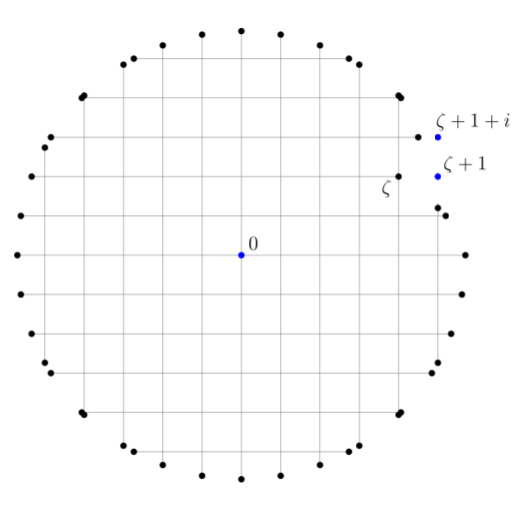
\includegraphics[width=9cm, height=9cm]{Omega_z.png}
  \centering
  \caption{Sketch of $\OZ$ for $\zeta = 4+2i$.  
    In Lemma \ref{Properties of H} (d), we will show that $\OZ$ is 
    close to the ball $B_{|\zeta|} \cap \mathcal{G}$.  
    The black dots are the boundary of $\OZ \subset \mathcal{G}$. 
    The lattice points $\zeta$, $\zeta+1$, and $\zeta+1+i$ are not 
    in $\OZ$.}
  \label{F: Omega_zeta}
\end{figure}

\begin{lemma}[Properties of $H^{\zeta}$]
  \label{Properties of H}
  There is a constant $C_1 < \infty$ 
  such that the following statements hold: 
  \begin{itemize}
    \item[(a)]   $ 1 \leq H^{\zeta}(\zeta), \;\;\;
      H^{\zeta}(\zeta + 1) < 0,  \;\;\;
      H^{\zeta}(\zeta+1+i) < 0, \;\;\; 
      H^{\zeta}(z) \leq 2$, \,\, for $\zeta \in K$ and all $z \in \mathcal{G}$, 

    \item[(b)] 
      $\zeta \in \partial \OZ$ and for 
      $z \in \partial \OZ \setminus \{ \zeta \}$ 
      it is $H^{\zeta}(z) = 1/(2 |\zeta|)$.

    \item[(c)] 
      $H^{\zeta}$ is grid-harmonic in $\OZ$. 

    \item[(d)] 
      $\mathbb{B}_{|\zeta|-C_1} \subset 
      \OZ \subset B_{|\zeta| + C_1}$

    \item[(e)] 
      For each $z \in \mathbb{B}_r$ with  $0\leq r < |\zeta| -C_1$ we have, 
      \begin{equation}\nonumber
        \frac{1}{2|\zeta|} \leq H^{\zeta}(z) 
          \leq \frac{1}{|\zeta| - r -C_1}.
      \end{equation}

    \item[(f)] For $0 \leq r \leq |\zeta|$ 
      we have the mean-value properties:  
      \begin{equation}\nonumber
        \bigg| \sum_{z \in \mathbb{B}_r} 
            \big( H^{\zeta}(z) -H^{\zeta}(0) \big) \bigg| 
          + \bigg| \sum_{z \in \OZ \cap \mathbb{Z}^2} 
              \big( H^{\zeta}(z) - H^{\zeta}(0) \big) \bigg|
        \leq C_1 \ln |\zeta|.
      \end{equation}
  \end{itemize}
\end{lemma}

Recall the definition of $F^{\zeta}$ given in \eqref{D: def F^zeta}. 
The next lemma allows us to derive some properties of $H^{\zeta}$ 
from $F^{\zeta}$, for instance from mean-value property (Theorem \ref{T: Mean-Value Formula}).
Lemma \ref{L: H close to F} will be our main factor in 
the proof of Lemma \ref{Properties of H} (d), (e), and (f).

\begin{lemma}[$H^{\zeta}$ is close to $F^{\zeta}$]
  \label{L: H close to F} 
  There is a constant $C_0 > 0$ such that for all $z \in \mathcal{G}$, 
  \begin{equation}
    \nonumber
    |H^{\zeta}(z) - F^{\zeta}(z)| 
      \leq \frac{C_0}{|\zeta - z|^2}
  \end{equation}
\end{lemma}

\begin{remark}
  Note the similarities between $H^{\zeta}$ and $F^{\zeta}$: 
  \begin{itemize}
    \item $F^{\zeta}$ is harmonic in $B_{|\zeta|}$, 
      $H^{\zeta}$ is grid-harmonic in $\OZ$ 
      (Lemma \ref{Propeties of F} \ref{p: F: harmonic} and Lemma \ref{Properties of H} (c));
    \item $F^{\zeta} = 1/(2|\zeta|)$ on $(\partial B_{|\zeta|}) \setminus \{\zeta\}$ and 
      $H^{\zeta} = 1/(2|\zeta|)$ on $(\partial \OZ) \setminus \{\zeta\}$, 
      see Lemma \ref{Propeties of F} \ref{p: F is shift of K} and Lemma \ref{Properties of H} (b); 
    \item $F^{\zeta}$ is invariant under rotation, 
      $H^{\zeta}$ is invariant under dihedral symmetries, see
      \eqref{eq: K invariant} and \eqref{eq: symmetries of H^zeta}. 
  \end{itemize}
\end{remark}

\begin{remark}
  $H^{\zeta}$ approximates the discrete Poisson kernel for the ball $\mathbb{B}_{|\zeta|}$  
  (that is the probability that a random walk started at $z \in \mathbb{B}_{|\zeta|}$ 
  exits the ball $\mathbb{B}_{|\zeta|}$ \hbox{in $\zeta$).} 
  The discrete Poisson kernel can be expressed in terms of potential kernels 
  $a(\mydot)$, see \cite{lawler} Lemma 6.3.6 and Proposition 4.6.2.
\end{remark}

We will make use of properties of the continuum Poisson kernel 
(Lemma \ref{Propeties of F}) and of the potential kernel 
(Lemma \ref{L: properties of a}) to prove Lemma \ref{Properties of H}. 

\begin{proof}[Proof of Lemma \ref{Properties of H}]
  \renewcommand{\qedsymbol}{}
  By the symmetries of $H^{\zeta}$, we may assume $\zeta \in K$.
  \begin{itemize}
    \item[(a)]
      Note that in the definition of 
      $H^{\zeta}$ the $\lambda_i$ are  
      the coefficients of the linear combination 
      of $\zeta /|\zeta|$ with respect to the basis $1$, $1+i$.
      Since $\zeta / |\zeta|$ is in the convex hull of 
      $\{0, 1, 1+i\}$, we have $\lambda_1, \lambda_2 \in [0,1]$ and 
      \begin{equation}\label{lambda1 plus lambda2}
        \lambda_1 + \lambda_2 \leq 1.
      \end{equation}

      Recall that by Lemma \ref{L: properties of a} (d),
      $a(1+i) = 4/ \pi$, $a(1) = 1$.
      Then, since $a(1+i) > a(1)$ , $\lambda_i \in [0,1]$, and Lemma \ref{L: properties of a} (c)
      (symmetries of the potential kernel) we see
      $H^{\zeta}(\zeta +1)$, 
      \hbox{$H^{\zeta}(\zeta +1+i) < 0$.}\\
      Since $a(\mydot)$ is subadditive (see Lemma \ref{L: properties of a} (e))  
      for any $z \in \mathbb{Z}^2$ it is 
      $a(z-\zeta-1) \leq$ \hbox{$a(z-\zeta) + a(1)$} and 
      $a(z-\zeta-1 -i) \leq$ \hbox{$a(z-\zeta) + a(1+i)$.} Hence, 
      using the exact values of $a(1)$ and $a(1+i)$, for any $z \in \mathbb{Z}^2$, 
      \begin{equation}\nonumber
        H^{\zeta}(z) 
        \leq \frac{\pi}{2} \big( \lambda_1 a(1) + \lambda_2 a(1+i) \big) 
        \leq 2(\lambda_1 + \lambda_2)
        \leq 2,
      \end{equation}
      where we used \eqref{lambda1 plus lambda2}. 
      Thus, by linearity $H^{\zeta}(z) \leq 2$ for all $z \in \mathcal{G}$. 
      On the other hand, 
      \begin{equation}\nonumber
        H^{\zeta}(\zeta) = 
        \frac{\pi}{2}\lambda_1 + 2 \lambda_2 
        \geq 
        \frac{\pi}{2}(\lambda_1 + \lambda_2)
          = \frac{\pi}{2} \text{Re} \frac{\zeta}{|\zeta|}\\
        \geq 
          \frac{\pi}{2} \text{Re} \frac{1+i}{|1+i|}
        > 1.  
      \end{equation}

    \item[(b)] 
      By (a) it is $H^{\zeta}(\zeta) >1> 1/(2\zeta)$ and
      the statement follows from the definition of $\OZ$. 

    \item[(c)]  
      By Lemma \ref{L: properties of a} the 
      only critical points are 
      $\zeta$, $\zeta + 1$, and $\zeta+1+i$.  
      However, by (a) and the definition of $\zeta$ these points are not in $\OZ$. 

    \item[(d)]
      For the first inclusion, $\mathbb{B}_{|\zeta| - C_1} \subset \OZ$, it suffices 
      to show $H^{\zeta}(z) > 1/(2|\zeta|)$ for all 
      \hbox{$z \in \partial B_{|\zeta|-C_1} \cap \mathcal{G}$} for some 
      constant $C_1 > 0$ (by Lemma \ref{L: maximum principle grid}).

      By Lemma \ref{L: H close to F}, there is a constant $C_0$, such that 
      \begin{equation}
        \nonumber
        H^{\zeta}(z) - F^{\zeta}(z) \geq - \frac{C_0}{|\zeta - z|^2},
      \end{equation}
      for all $z \in \mathcal{G}$. 
      Choosing $C_1 := 28C_0$ and $C := 2C_0$ in \hbox{Lemma \ref{L: F on B_zeta+14C}}, %change these constants if Lemma \ref{L: F on B_zeta+14C} changes
      leads to 
      \begin{equation}\nonumber
        F^{\zeta}(z) - \frac{1}{2|\zeta|} \geq \frac{2C_0}{|\zeta-z|^2},
      \end{equation}
      for all $z \in \partial B_{|\zeta|-C_1} \cap \mathcal{G}$. 
      Combining both inequalities,
      \begin{equation}\nonumber
      \begin{split}
        H^{\zeta}(z) - \frac{1}{2|\zeta|} 
        &=  H^{\zeta}(z)-F^{\zeta}(z)+F^{\zeta}(z) - \frac{1}{2|\zeta|}\\
        &\geq -\frac{C_0}{|\zeta - z|^2}  
              +\frac{2 C_0}{|\zeta - z|^2} > 0.
      \end{split}
      \end{equation}
      Using maximum principle for grid-harmonic functions, Lemma \ref{L: F on B_zeta+14C}, 
      and Lemma \ref{L: H close to F} and the same choices of $C_1$ and $C$, it is for 
      all $z \in B_{|\zeta|+C_1} \cap \mathcal{G}$,
      \begin{equation*}
        \begin{split}
          H^{\zeta}(z) - \frac{1}{2|\zeta|} 
          & =  H^{\zeta}(z) - F^{\zeta}(z) + F^{\zeta}(z) - \frac{1}{2|\zeta|} \\
          & \leq \frac{C_0}{|\zeta - z|^2} - \frac{2C_0}{|\zeta-z|^2} 
          < 0, 
        \end{split}
      \end{equation*}
      which proves the inclusion $\OZ \subset B_{|\zeta|+C_1}$.

    \item[(e)]
      By (d) it is $\mathbb{B}_r \subset \OZ$, hence 
      the lower bound follows by the definition of $\OZ$.\\
      For the upper bound use Lemma \ref{L: H close to F} and 
      Lemma \ref{Propeties of F} \ref{p: sup F^zeta over B_r}, to get
      \begin{equation}\nonumber
        \begin{split}
          \max_{z \in \mathbb{B}_r} H^{\zeta}(z) 
           \leq \sup_{z \in B_r} F^{\zeta}(z) + \sup_{z \in B_r} \frac{C_0}{|\zeta - z|^2}
          &\leq \frac{1}{|\zeta| - r} + \frac{C_0}{(|\zeta| - r)^2}\\
          &\leq \frac{1}{|\zeta|-r -C_1},
        \end{split} 
      \end{equation}
      where the last inequality holds by the choice $C_1 = 28 C_0$ we made in 
      the proof of (d). %change if C changes

    \item[(f)] 
      At first assume $0 < r \leq |\zeta| - C_1$.
      By mean-value property \hbox{(Theorem \ref{T: Mean-Value Formula})}
      we have, 
      \begin{equation} \label{F mean val prop}
        \int_{B_r} \big( F^{\zeta}(z) - F^{\zeta}(0) \big) 
        = 0,
      \end{equation} 
      since $F^{\zeta}$ is harmonic in $B_r$.
      Using Lemma \ref{L: H close to F}, we will approximate 
      \begin{equation}\label{mean val of H}
        \sum_{z \in \mathbb{B}_r} 
          \big( H^{\zeta}(z) - H^{\zeta}(0) \big) 
      \end{equation} 
      by \eqref{F mean val prop}, and get an error of order $\ln |\zeta|$. 
      For this approximation we proceed in three steps. 
      At first, we see that by Lemma \ref{L: H close to F},
      \begin{equation}\nonumber
        \begin{split}
          \bigg|& \sum_{z \in \mathbb{B}_r} 
            \big( H^{\zeta}(z) - H^{\zeta}(0) \big) 
          - \sum_{z \in \mathbb{B}_r} 
              \big(F^{\zeta}(z) - F^{\zeta}(0) \big) \bigg|\\
          &\leq  \sum_{z \in \mathbb{B}_r} 
          \bigg( \frac{C_0}{|\zeta - z|^2} + \frac{C_0}{|\zeta|^2} \bigg)
          \leq 8 \pi C_0 \ln |\zeta|.
        \end{split}
      \end{equation}
      Second, if $\square_z$ denotes the unit square 
      with center in $z \in \mathbb{Z}^2$ and 
      \begin{equation}\nonumber
        B^{\square}_r := \bigcup_{z \in \mathbb{B}_r} \square_z,
      \end{equation} 
      then Lemma \ref{Propeties of F} \ref{p: sup of F^zeta on small circles}
      implies 
      \begin{equation}\nonumber
        \sup_{\omega \in \square_z} F^{\zeta}(\omega) -F^{\zeta}(z)
        \leq \frac{2}{|\zeta - z|^2}. 
      \end{equation}
      Hence,
      \begin{equation}\nonumber
      \begin{split}
      \bigg| \int_{B^{\square}_r} F^{\zeta}(z) dz 
          - \sum_{z \in \mathbb{B}_r} F^{\zeta}(z)\bigg|
      &= \bigg| \sum_{z \in \mathbb{B}_r} 
              \int_{\square_z}
              \big(F^{\zeta}(\omega) -F^{\zeta}(z)\big) 
              d \omega \bigg|\\
      &\leq \sum_{z \in \mathbb{B}_r} 
            \frac{2}{|\zeta - z|^2} \\
      &\leq 8 \pi \ln |\zeta|.
      \end{split}
      \end{equation}
      Third, 
      \begin{equation}\nonumber
      \begin{split}
      \bigg| \int_{B_r^{\square}} F^{\zeta}(z) \;dz 
          - \int_{B_r} F^{\zeta}(z) \; dz \bigg| 
      &= \bigg| \int_{B_{r+1} \setminus B_{r-1}} 
        F^{\zeta}(z) \;dz \bigg| \\ 
      &\leq \int_{B_{r+1} \setminus B_{r-1}} 
        \frac{1}{|\zeta-z|} \; dz\\
      &= \int_0^{2\pi} \int_{r-1}^{r+1} 
        \frac{1}{|s e^{i \theta} - \zeta|} s \;ds \;d\theta \\
      &\leq 4 \int_0^{2\pi} 
      \frac{1}{|r e^{i \theta} - \zeta|} r \; d\theta \\
      &\leq 8 \int_{\alpha}^{\alpha + \pi} 
        \Big( \frac{d}{d\theta} 
        \ln |re^{i \theta} -\zeta| \Big) \;d\theta\\
      &\leq 8 \pi \ln |\zeta|,
      \end{split}  
      \end{equation}
      where $\alpha$ denotes the angle for which 
      $r e^{i \alpha}$ has minimal distance to $\zeta$.
      In addition, 
      \begin{equation}\nonumber
        \bigg| \int_{B_r} F^{\zeta}(0) \;dz 
            - \sum_{z \in \mathbb{B}_r} F^{\zeta}(0)\bigg| 
        = \frac{|\pi r^2 - |\mathbb{B}_r||}{|\zeta|} 
        \leq 9.
      \end{equation}
      Using this, the three steps above,  
      and \eqref{F mean val prop}, the result can be derived. 

      It remains to prove the approximate 
      mean-value property for $\mathbb{B}_r$, 
      when $|\zeta| - C_1 \leq r < |\zeta|$, 
      and for $\Omega_{\zeta} \cap \mathbb{Z}^2$. 
      By (e) we have
      $\mathbb{B}_{|\zeta|-C_1} \subset \OZ \cap \mathbb{Z}^2 
      \subset \mathbb{B}_{|\zeta|+C_1}$; 
      therefore, the sum \eqref{mean val of H}
      differs at most by the lattice points in the annulus 
      $R=\mathbb{B}_{|\zeta| +C_1} \setminus \mathbb{B}_{|\zeta| - C_1}$, i.e., by 
      \begin{equation}\nonumber 
        \begin{split}
          \sum_{z \in R} \big( |H^{\zeta}(z)| + |H^{\zeta}(0)| \big) 
          &\leq  \sum_{z \in R} 
              \min \bigg( \frac{2}{|\zeta - z|}, 2 \bigg)
              + |R| \frac{2}{|\zeta|}\\
          &\leq 32 \pi C_1 \ln |\zeta|,
        \end{split}
      \end{equation} 
      where we used $H^{\zeta} \leq 2$ (see Lemma \ref{Properties of H} (a)), 
      Lemma \ref{L: H close to F}, and $|R| \leq 16 C_1 |\zeta|$. 
      This completes the proof. 
  \end{itemize}
\end{proof}


\begin{proof}[Proof of Lemma \ref{L: H close to F}]
  \renewcommand{\qedsymbol}{}
  This result is based on the approximation \hbox{$a(z) \approx \ln |z|$} 
  (see Lemma \ref{L: properties of a} (b)).
  Here the choice of the coefficients 
  $\lambda_1$, $\lambda_2$ comes into play.

  By Lemma \ref{L: properties of a} (b) 
  we can see that 
  \begin{equation}\label{eq:H = ln}
  \begin{split}
        H^{\zeta}(z)& - \big(\lambda_1 ( \ln |z-\zeta -1| -\ln |z-\zeta|)
                + \lambda_2 ( \ln |z-\zeta -1-i| -\ln |z-\zeta|) \big)\\
      &= O \bigg( \frac{1}{|\zeta - z|^2} \bigg).
    \end{split}
    \end{equation}
    Then if $\gamma$ denotes the 
    line segment from $z-\zeta$ to $z - \zeta -1$, we get
    \begin{equation}\nonumber
    \begin{split}
      \ln |z-\zeta -1| -\ln |z-\zeta|
    &= \text{Re} \int_{\gamma} \frac{1}{\omega}\\
    &= - \int_0^1 \text{Re} \frac{1}{z-\zeta-t} dt \\
    &= \text{Re} \frac{1}{z-\zeta} + 
        O\bigg( \frac{1}{|z - \zeta|^2} \bigg),
  \end{split}
  \end{equation}
  where for the last equality we used the Taylor series in $t=0$. 
  Plugging this (and the analog for $\ln |z-\zeta -1-i| -\ln |z-\zeta|$)
  into Equation \eqref{eq:H = ln} above, we get
  \begin{equation}\nonumber
    \begin{split}
    &\lambda_1 ( \ln |z-\zeta -1| -\ln |z-\zeta|)
    + \lambda_2 ( \ln |z-\zeta -1-i| -\ln |z-\zeta|) \\
    &= -\lambda_1 \text{Re} \frac{1}{z-\zeta} 
      -\lambda_2 \text{Re} \frac{1+i}{z-\zeta}  
      +  O\bigg( \frac{1}{|z - \zeta|^2} \bigg)\\
    &= F^{\zeta} + O\bigg( \frac{1}{|z - \zeta|^2} \bigg).
    \end{split}
  \end{equation} 
  This finishes the proof. 
\end{proof}


\section{Grid IDLA}
In order to define a continuous martingale, we introduce 
a growth model similar to the IDLA, where 
the underlying particles are grid Brownian Motions. 
The martingale will be defined by the values of 
$H^{\zeta}$ on those particles. To ensure the martingale 
property, the particles are stopped on 
exiting $\OZ$, i.e., before 
reaching a point where harmonicity of $H^{\zeta}$ fails.


\subsection{Definition}
\label{sec: grid idla}
Define a process $\AZT$,  $t \geq 0$ on the grid, 
which for $t$ being an integer, behaves like the IDLA process on 
$\mathbb{Z}^2$.\\~\\
We let  
\begin{equation}\label{D: set S}
  S :=(\Omega_{\zeta} \cap \mathbb{Z}^2) \cup \partial \Omega_{\zeta}
\end{equation}
denote the lattice points in $\Omega_{\zeta}$ and its boundary in $\mathcal{G}$.
Let $\tilde{\beta}^1$, $\tilde{\beta}^2$, $\tilde{\beta}^3$, ...  
be independent grid Brownian motions and
$$\tau^n = 
  \begin{cases}
    0 &, n=1\\
    \text{inf}
       \{t \geq 0 \,|\,
         \tilde{\beta}^n(t) \in (\mathbb{Z}^2 \setminus \AZN) \cup \partial \OZ \}  &,
           n \geq 2
\end{cases}$$
be the first time the $n$th grid Brownian motion
either reaches the boundary of $\OZ$ or hits a lattice point (in $\OZ$), 
which is not already occupied by $\AZN$.
Define the 
time change $s \mapsto s'' := \frac{s}{1-s}$, $\;[0,1) \rightarrow \mathbb{R}$.
For each $n$ define a time-changed and stopped grid BM by
\begin{equation}\label{D: time changed grid BM}
  \beta^n(s) = \tilde{\beta}^n(s'' \land \tau^n),
\end{equation}
for $s \in [0,1)$. Note that a.s.
$\beta^n(1) = \lim\limits_{s \rightarrow 1}{\beta^n(s)}
   = \tilde{\beta}^n(\tau^n)$ .
For $t \in [0,1]$ define the \textbf{grid IDLA} $\AZT$ by
\begin{equation}
  \label{D: AZT}
  \nonumber
  \AZT = \big( \beta^1(t) \big),
\end{equation}
and for $t \in (n,n+1]$ define 
  $\AZT : \Omega \rightarrow S^{n} \times \bar{\Omega}_{\zeta}$ 
by
\begin{equation}\label{D: AZT, real def}
  \nonumber
 \AZT =  
  \big( 
    \beta^1(1),...,\beta^{n}(1),\beta^{n+1}(t-n)
  \big).
\end{equation}
We will refer to $A^{\zeta}$ in different ways: 
if it occurs in the context of set operators, 
as in the definition of $\tau^n$, we refer to $A^{\zeta}$ as a set;
if we iterate over $A^{\zeta}$, we refer to $A^{\zeta}$ as a multiset. 

\begin{remark}
  The first particles of $A^{\zeta}$ 
  are either lattice points or on the boundary of $\OZ$; 
  the last particle can be somewhere in $\bar{\Omega}_{\zeta}$. 
  Hence, although not generally, the set $A^{\zeta}$ is 
  increasing over integer time steps.
  Moreover, points of $A^{\zeta}$ in $\OZ$ are almost surely
  of multiplicity at most one; however, at the boundary $\partial \OZ$ 
  the grid IDLA may have points of larger multiplicity. 
\end{remark}


\subsection{Main Martingale} 
\label{sec: define the martingale}
In this section we introduces a process that plays a crucial
role in the proof of Theorem \ref{log fluctuation}. 
Showing that this process is a martingale (Lemma \ref{lemma M : martingale}), 
is the main result of this section.\\~\\
Let $t \in (n,n+1]$. For $i \in \{1,...,n+1\}$ let $\pi^i$ be 
the projection on the $i$th coordinate. 
Then $\MZT : \Omega \rightarrow \mathbb{R}$ can be defined by
\begin{equation}
  \label{D: MZT}
  \MZT = \sum_{i=1}^{n+1} f \big( \pi^i(\AZT) \big) 
          = \sum_{i=1}^{n} f \big(\beta^i(1) \big) + f \big(\beta^{n+1}(t-n) \big),
\end{equation}
where 
  $$f: \mathcal{G} \rightarrow \mathbb{R}, \quad f(z) = H^{\zeta}(z)- H^{\zeta}(0).$$
Multiset notation enables us to write  
 $$
  M^{\zeta}(t) = \sum_{z \in A^{\zeta}(t)} f(z).
 $$

\begin{lemma}
  \label{lemma M : martingale}
  $M^{\zeta}$ is a martingale w.r.t. 
  $\mathcal{F}_t = \sigma(A^{\zeta}(s) \,|\, 0 \leq s \leq t)$.
\end{lemma}

\begin{lemma}\label{L: M as BM}
  $M^{\zeta}$ can be written as a time change 
  $t \mapsto \QVT$ of a standard Brownian motion $\mathcal{B}$, i.e.,
  \begin{equation}\nonumber
    \MZT = \mathcal{B}(\QVT).
  \end{equation}
\end{lemma}

\begin{remark}
  If $T_s = \inf \{ t \geq 0 \,|\, \langle M^{\zeta} \rangle _t \geq s \}$
  denotes the time at which $\langle M^{\zeta} \rangle$ reaches $s$, 
  then the time change $\langle M^{\zeta} \rangle _t\,$, $t \geq 0$
  is a family of stopping times with respect to 
  $(\mathcal{F}_{T_s})_{s \geq 0}$. Furthermore, the BM $\mathcal{B}$ is adapted 
  to the filtration $\mathcal{F}_{T_s}$.
\end{remark}

\begin{proof}[Proof of Lemma \ref{L: M as BM}]
  \renewcommand{\qedsymbol}{}
  Show that $M^{\zeta}$ satisfies the assumptions 
  of Theorem \ref{theorem DDS}; 
  then the result follows.

  We have seen that $M^{\zeta}$ is a continuous martingale. 
  $M^{\zeta}$ clearly vanishes in $t=0$.
  It remains to show that $\langle M \rangle _ {\infty} = \infty$.
  Remember that $M^{\zeta}$ is the sum of $H^{\zeta}$ over the  
  particles of $A^{\zeta}$. The particles
  act like Brownian motions on the edges of $\mathcal{G}$,   
  and $H^{\zeta}$ is linear on the edges.  
  Since for a BM $\mathcal{B}$,   
  \begin{equation}\nonumber
    \lim_{t \rightarrow \infty} \langle \mathcal{B} \rangle _t 
    = \lim_{t \rightarrow \infty} t = \infty,
  \end{equation}
  we can conclude $\langle M \rangle _ {\infty} = \infty$.
\end{proof}


\begin{proof}[Proof of Lemma \ref{lemma M : martingale}]
  Fix $\zeta \in \mathbb{Z}^2$ and let $f$, $S$, and $\mathcal{F}_t$ be defined 
  as above in this section.
  Let $t \in$ \hbox{$(n, n+1]$} and regard $A^{\zeta}$ as a process 
  \mbox{$\AZT : (\Omega, \mathcal{F}_t) \rightarrow 
    (S^{n} \times \bar{\Omega}_{\zeta},\,
    \mathcal{P}(S^{n}) \otimes 
    \mathcal{B}(\bar{\Omega}_{\zeta}) )$. }

  Since $f$ and the projections $\pi^i$ are measurable, 
  $\MZT$ is adapted to $\mathcal{F}_t$.
  Moreover, $f$ is bounded on $\bar{\Omega}_{\zeta}$, 
  and since we sum over $n+1$ many 
  particles in $\bar{\Omega}_{\zeta}$ at time $t$, it is 
  \mbox{$\Ex( |\MZT| ) < \infty$.}

  Now prove the martingale property.
  Theorem \ref{harmonic function of grid BM} states
  that grid-harmonic functions of 
  grid Brownian motions are martingales.
  This will be our key argument. 

  By an iteration of tower property  
  it suffices to show 
  \begin{equation}\nonumber
    \Ex( \MZT \,| \, \mathcal{F}_s) = M^{\zeta}(s),
    \;\;\;\text{for}\; s \in [n, t).
  \end{equation} 
  Moreover, since $M^{\zeta}(n)$ is 
  $\mathcal{F}_{n} \subset \mathcal{F}_s$ measurable, 
  it is
  \begin{equation}\nonumber
  \begin{split}
  \Ex(\MZT \,|\, \FS) 
  & = \Ex \bigg( 
          \sum_{i=1}^{n} f \big( \pi^i(A^{\zeta}(n)) \big)
          + f \big( \pi^{n+1}(\AZT) \big) \,\bigg|\, \FS \bigg)\\
  & = M^{\zeta}(n) + 
    \Ex \big(f(\beta^{n+1}(t-n)) \,\big|\, \FS \big).
  \end{split}
  \end{equation}
  So it suffices to prove that
  $$\Ex \big( f(\beta^{n+1}(t-n)) \, \big| \, \FS \big) 
    = f( \beta^{n+1}(s-n)).$$ 
  The notation
  $\beta^{n+1}(u) = \tilde{\beta}^{n+1}(\frac{u}{1-u} \land \tau^{n+1})$
  for $u \in [0,1]$
  refers to the definition of the grid 
  IDLA \eqref{D: time changed grid BM}.
  For simplicity denote 
  $\beta := \beta^{n+1}$, 
  \hbox{$\tilde{\beta} := \tilde{\beta}^{n+1}$}, 
  and $\tau := \tau^{n+1}$. 
  Let $t' := t-n, \, s':= s-n$ be the shifted times 
  in the domain of 
  $\beta$, and
  $t'' := \frac{t'}{1-t'}, \, s'':= \frac{s'}{1-s'}$ 
  the accelerated times used for the definition 
  of the grid Brownian motion. Obtain 
  that the last grid BM $\beta(t')$ only depends on its own 
  history and on $\AZN$; 
  the trajectory of $A^{\zeta}(\mydot)$ up to time 
  $n$ does not have any effect. Hence,
  \begin{equation}
    \nonumber
    \begin{split}
      \Ex & \big(  f(\beta(t')) \,\big|\, \FS \big) \\
      & = \Ex \big( 
        f(\beta(t')) 
          \, \big|\, \mathcal{F}_n, \, \beta(u) \,: 0 \leq u \leq s' \big)\\
      & = \Ex \big( 
        f(\beta(t')) 
          \, \big|\, \AZN , \, \beta(u) \,: 0 \leq u \leq s' \big)\\
      & = \Ex \big( f(\tilde{\beta}(t'' \land \tau))  
        \,\big|\, \AZN ,\, \tilde{\beta}(u \land \tau) \,:
          0 \leq u \leq s''\big) \\
      & = \sum_{A \in S^{n}} 
            \Ex \big( f(\tilde{\beta}(t'' \land \tau) )  
            \, \big|\, \AZN = A,\, \tilde{\beta}(u) \,:
              0 \leq u \leq s''\big) \cdot \boldsymbol{1}_{\{\AZN = A\}}.
    \end{split}
  \end{equation}
  For the last equality note that $|S^n| < \infty$, where the set $S$ is as in \eqref{D: set S}. 
  Next we apply Theorem \ref{harmonic function of grid BM} 
  on each summand of the equation above; 
  for this note that on the event 
  $\{ \AZN = A\}$ the time $\tau$, which stops $\tilde{\beta}$ on hitting 
  $\partial \OZ \cup (\mathbb{Z}^2 \setminus A)$, equals the exit time 
  $\tau_{\tilde{A}} = \inf \{t \geq 0 \,|\,
    \tilde{\beta}(t) \notin \tilde{A} \}$,
  where $\tilde{A} \subset \mathcal{G}$ is an 
  open set constructed by the union of the open crosses $z+E$ with
  centers that are the lattice points of $A$: 
  \begin{equation}\nonumber
    \tilde{A} = 
    \OZ \cap \bigcup_{z \in A \cap \mathbb{Z}^2} 
      (z + E).
  \end{equation}
  Since $H^{\zeta}$ is grid-harmonic in 
  $\OZ$ and $\tilde{A} \subset \OZ$,
  we can conclude that
  $f$ is grid-harmonic on $\tilde{A}$ and we can apply 
  Theorem \ref{harmonic function of grid BM}
  (see also the remark of Theorem 
  \ref{harmonic function of grid BM}). 
  Hence, on the event $\{\AZN = A \}$ we get
  \begin{equation}
    \nonumber
    \begin{split}
      \Ex \big( & f(\tilde{\beta}(t'' \land \tau) )  
          \, \big|\, \AZN = A,\, \tilde{\beta}(u) \,:
            0 \leq u \leq s'' \big)\\
      & = 
        \Ex \big( f(\tilde{\beta}(t'' \land \tau_{\tilde{A}}) )  
      \,\big|\, \AZN = A,\, \tilde{\beta}(u) \,:
      0 \leq u \leq s'' \big)\\
      & = 
        \Ex \big( f(\tilde{\beta}(t'' \land \tau_{\tilde{A}}) )  
        \,\big|\, \tilde{\beta}(u) \,:
        0 \leq u \leq s'' \big) \\
      & = 
      f(\tilde{\beta}(s'' \land \tau_{\tilde{A}}))\\
      & = f(\beta(s')).
    \end{split}
  \end{equation}
  In total this gives us
  $\, \Ex( f(\beta^{n+1}(t')) \,|\, \FS) = f(\beta^{n+1}(s'))$.
\end{proof}


\section{Logarithmic Fluctuations} 
\label{Sec: Proof Lof Fluctuation}
The aim of this section is to prove Theorem 
\ref{log fluctuation} on a high level, i.e., only using the 
lemmas \ref{No Very Late Point}, \ref{Early Points Imply Late Points}, 
and \ref{Late Points Imply Early Points}
that are about the occurrence of early and late points.
While stated here, we will prove these lemmas 
in Section \ref{sec: detect early and late points}.
We begin with an a priori bound on the probability of very late points.

\begin{lemma}[No very late point] 
  \label{No Very Late Point}
  There are constants $C_2$, $c_2 > 0$ 
  such that if $T \geq 100 \pi$
   and $l \geq \sqrt{\frac{T}{100 \pi}}$, then 
  $$
  \mathbb{P} \big( \mathcal{L}^{l}(T) \big) 
  \leq C_2 e^{-c_2 \sqrt{T}}.
  $$
\end{lemma}

Fix $\gamma > 1$ and define the constants
\begin{equation}\nonumber
  \begin{split}
    &C_3 = \max \{(\gamma + 5 + \ln C_2 )/c_2 ,\; C_1 1000/b \},\\
    &C_4 = \Big(2700 + \frac{1}{c_2} \Big)(\gamma + 3)
      +\frac{2 \ln C_2}{c_2} + 2C_1 +2,
  \end{split}
\end{equation}
where $C_1$ and $b$ are as defines in Lemma \ref{Properties of H} 
and Lemma \ref{No Thin Tentacles}.

\begin{lemma}[Early points imply late points]
  \label{Early Points Imply Late Points}
  Fix $T \geq 19$. Then for all $l$ and $m$ 
  satisfying $m \geq C_3 \ln T$ and $l \leq (b/1000)m$, 
  $$
  \mathbb{P} \big( \mathcal{E}^m(T) \cap \mathcal{L}^l(T)^c \big)
  \leq T^{-(\gamma + 1)}.
  $$
\end{lemma}

\begin{lemma}[Late points imply early points]
  \label{Late Points Imply Early Points}
  If $l$, $m \in \mathbb{N}$ 
  such that \hbox{$l \geq C_4 \ln T$} and 
  \mbox{$m \leq l^2 / (C_4 \ln T)$}, then 
  $$
  \mathbb{P} \big( \mathcal{L}^l(T) \cap \mathcal{E}^m(T)^c \big) 
    \leq T^{-(\gamma + 1)}.
  $$
\end{lemma}

\begin{remark}
  In Theorem \ref{log fluctuation} 
  (see also Lemma \ref{L: logarithmic fluctuation in terms of late and early points})
  $l$ can be chosen much smaller than 
  in Lemma \ref{No Very Late Point}, which bounds 
  the probability of an $l$-late point for $l$ being of order $\sqrt{T}$.
\end{remark}


\subsection{Proof of Theorem \ref{log fluctuation}} 
\label{sec: high level proof of log fluct}
This section contains the proof of Theorem \ref{log fluctuation} 
with the help of the lemmas above. 
We begin with a brief overview of the proof.\\~\\
We define sequences of $l$ and $m$ for which $l$-late and $m$-early points 
are unlikely. Lemma \ref{No Very Late Point} states that 
$\sqrt{T}$-late points are unlikely.
Hence, we start with $l$ being of order $\sqrt{T}$ and
choose (according to Lemma \ref{Early Points Imply Late Points} 
and \ref{Late Points Imply Early Points}) 
iteratively smaller values for $l$ and $m$; 
we end up with $l$ and $m$ being of order $\ln T$.
While the assumptions $m \geq C_3 \ln T$ and $l \geq C_4 \ln T$ 
(of Lemma \ref{Early Points Imply Late Points} and Lemma \ref{Late Points Imply Early Points})
give an absolute lower bound on how much $l$ and $m$ may decline,
the assumptions $l \leq \frac{b}{1000} m$ and $m \leq l^2/(C_4 \ln T)$ 
bound how much $m$ and $l$ may decrease with each iteration.
The absolute lower bounds will eventually determine the 
logarithmic fluctuations. 

\begin{proof}[Proof of Theorem \ref{log fluctuation}]
  \renewcommand{\qedsymbol}{}
  Fix $\gamma > 1$.  
  Lemma \ref{L: logarithmic fluctuation in terms of late and early points} tells us that
  it suffices to find a constant $a$ and some $l, m < a \,\ln r$ such that 
  \begin{equation}\label{eq: lemma rephares log fluc in terms of early and late points}
    \mathbb{P} \big( \mathcal{L}^l(T)\big) 
    +\mathbb{P} \big( \mathcal{E}^m(T)\big)
    \leq r^{-\gamma}.
  \end{equation}
  To proof this, we use an iteration procedure.

  Fix $T > 100  \pi$.
  Start the iteration by choosing $l_0$ according to 
  Lemma \ref{No Very Late Point}, i.e.,
  $l_0 := \sqrt{T/(100 \pi)}$. Thus, 
  \begin{equation}\label{eq: no l_0 late point}
    \mathbb{P} \big( \mathcal{L}^{l_0}(T) \big) \leq C e^{-c \sqrt{T}}
    \leq T^{-(\gamma + 1)} 
  \end{equation}
  holds. Provided $l_i$ is fixed, we choose $m_i$ 
  according to Lemma \ref{Early Points Imply Late Points}'s 
  assumption $l \leq m\, b/1000$, 
  and provided $m_i$ is fix, we choose $l_{i+1}$ according Lemma \ref{Late Points Imply Early Points}, 
  i.e., for $i \geq 0$ we define alternating recursively 
  \begin{equation} \label{eq: def of l_i, m_i}
    \begin{split}
      & m_i :=  \frac{1000}{b} l_i,\\
      & l_{i+1} := \sqrt{ m_i C_4 \ln T },
    \end{split} 
  \end{equation}
  i.e, each element of the sequence 
  $l_{i}$ (and also $m_{i}$) decays like the square root 
  of its predecessor.
  Since
  \begin{equation}\nonumber
    \mathbb{P} \big( \mathcal{E}^{m_i}(T) \big) 
    \leq 
    \mathbb{P} \big( \mathcal{E}^{m_i} (T) \cap 
    \mathcal{L}^{l_i}(T)^c \big) + 
    \mathbb{P} \big(\mathcal{L}^{l_i}(T) \big),
  \end{equation}
  Lemma \ref{Early Points Imply Late Points} states that the occurrence of 
  an $m_i$-early point is unlikely if an $l_i$-late point is unlikely. 
  Hence, using \eqref{eq: no l_0 late point}, 
  \begin{equation}\label{eq: first step m_0}
    \mathbb{P}(\mathcal{E}^{m_0}(T)) 
    \leq 2T^{-(\gamma +1)}.  
  \end{equation}
  Similarly, we use 
  \begin{equation}\nonumber
    \mathbb{P} \big( \mathcal{L}^{l_{i+1}}(T) \big) 
    \leq 
    \mathbb{P} \big( \mathcal{L}^{l_{i+1}} (T) \cap 
    \mathcal{E}^{m_i}(T)^c \big) + 
    \mathbb{P} \big(\mathcal{E}^{m_i}(T) \big)
  \end{equation}
  with Lemma \ref{Late Points Imply Early Points} and \eqref{eq: first step m_0}, to get 
  \begin{equation}\label{eq: first step with l_1}
    \begin{split}
        \mathbb{P} \big(\mathcal{L}^{l_1}(T) \big) 
        & \leq \mathbb{P} \big(
          \mathcal{L}^{l_1}(T) \cap \mathcal{E}^{m_0}(T)^c \big) 
          +  \mathbb{P}(\mathcal{E}^{m_0}(T) \big)\\
      & \leq T^{-(\gamma +1)} + 2T^{-(\gamma +1)}.  
    \end{split}
  \end{equation}
  By induction we derive directly from definition
  \begin{equation}\label{eq: non recursive form}
    \begin{split}
      & l_i = \alpha^{1-1/2^i}\, l_0^{1/2^i},\\
      & m_i = \alpha^{1-1/2^i}\, m_0^{1/2^i},
    \end{split}
  \end{equation} 
  where $\alpha := (1000/b) C_4 \ln T$.

  Define 
  $$C_5 = \max \{ 1,  1000/b\} \cdot \max \{ C_3, C_4\}.$$ 
  We claim that for the sequences 
  $l_i$ and $m_i$ and for $a := 3C_5$ there is a $k = k(T)$
  such that 
  \begin{itemize}
    \item[\textbf{(i)}] for all $n \leq k$ it is 
      $l_n \geq C_4 \ln T$ and 
      $m_n \geq C_3 \ln T$, 
    \item[\textbf{(ii)}] $l_k, m_k \leq a \ln T$ 
        (i.e., fluctuation is at most logarithmic), and
    \item[\textbf{(iii)}] $k << \ln T$ 
      (i.e., the upper bounds on $\mathbb{P}\big(\mathcal{L}^{l_k}(T)\big)$ 
      and $\mathbb{P}\big(\mathcal{E}^{l_k}(T)\big)$ are not weakened too much).
  \end{itemize} 
  The following sketch outlines the constraints (i), (ii), and (iii).
  \begin{figure}[H] \label{valid vals l_k}
    \captionsetup{width=.8\linewidth}
    \begin{tikzpicture}
      % horizontal axis
      \draw[->] (0,0) -- (10,0) node[anchor=north] {$i$};
      % labels
      \draw	(0,3.1)  node[anchor=east] {$a \ln T$}
            (0,1.4) node[anchor=east] {$C_4 \ln T$}
            (0,2.5) node[anchor=east] {$l_k$};
      \draw (4,0) node[anchor=north] {$k$}
            (8,0) node[anchor=north] {$\ln T$};
      \draw	(0,-0.2)  node[anchor=east] {$0$};
      % vertical axis
      \draw[->] (0,0) -- (0,5) node[anchor=east] {$l_i$};
      % helper lines
      \draw [dotted] (0, 3) -- (9.5, 3);
      \draw [dotted] (0, 1.5) -- (9.5, 1.5);
      \draw[dotted] (3.4,0) -- (3.4,3);
      \draw[dotted] (6.4,0) -- (6.4,1.5);
      \draw[dotted, thick] (4,0) -- (4, 2.6);
      \draw[dotted, thick] (0,2.6) -- (4,2.6);
      \draw (8,0) -- (8,0.1);
      \draw (4,0) -- (4,0.1);
      % graph
      \draw[thick] (1,5) parabola[bend at end] (9,1.1);
    \end{tikzpicture}
    \caption{This sketch illustrates the decline of $l_i$ over $i$, i.e., 
      with each step we prove a smaller fluctuation from circularity to the inside.
      The dotted vertical lines mark the valid range for $k$ (see (i), (ii), and (iii)).}
  \end{figure}
  By (i) the assumptions of Lemma \ref{Early Points Imply Late Points}
  and Lemma \ref{Late Points Imply Early Points} are fulfilled for all $l_n$, $m_n$ with $n < k$.
  Hence, we can inductively repeat the steps \eqref{eq: first step m_0} 
  and \eqref{eq: first step with l_1}, which gives us
  \begin{equation}\nonumber
    \begin{split}
      & \mathbb{P} \big( \mathcal{L}^{l_k}(T) \big) 
          \leq (2k+1) T^{-(\gamma + 1)}, \; \; \text{and}\\
      & \mathbb{P}(\mathcal{E}^{l_k}(T)) 
      \leq (2k+2) T^{-(\gamma + 1)}.
    \end{split}
  \end{equation}
  Therefore, using (ii) and (iii),
  \begin{equation}\nonumber
  \begin{split}
    \mathbb{P} \big(\mathcal{L}^{a \ln T}(T) \big)
    & \leq \mathbb{P}\big(\mathcal{L}^{l_k}(T) \big)\\
    & \leq (2k+1) T^{-(\gamma + 1)} \\
    & \leq \frac{1}{2} T^{-\gamma}, 
  \end{split}
  \end{equation}
  for $T$ sufficiently large. With the same arguments,
  \begin{equation}\nonumber
  \begin{split}
    \mathbb{P} \big(\mathcal{E}^{a \ln T}(T) \big)
      \leq \frac{1}{2} T^{-\gamma}. 
  \end{split}
  \end{equation}
  We rephrase the fluctuation bounds in terms of the radius $r$ instead of the time $T = T(r):= \pi r^2$.
  Note that
  $$
    3a \ln r \geq a \ln T,
  $$
  for $r$ sufficiently large, i.e., mapping $r$ to $T$ changes the fluctuation only by a constant factor. 
  Hence, we have
  \begin{equation} \nonumber
  \begin{split}
    \mathbb{P} (\mathcal{E}^{3a \ln r}(T)) 
      + \mathbb{P} (\mathcal{L}^{3a \ln r}(T)) 
    & \leq \mathbb{P} (\mathcal{E}^{a \ln T}(T)) 
      + \mathbb{P} (\mathcal{L}^{a \ln T}(T)) \\
    & \leq \frac{1}{2} T^{-\gamma} + \frac{1}{2} T^{-\gamma} \\
    & \leq r^{-\gamma},
  \end{split}
  \end{equation}
  which by \eqref{eq: lemma rephares log fluc in terms of early and late points} 
  proves the theorem. 

  It remains to prove the existence of a $k=k(T)$ such that (i), (ii), and (iii) hold. 
  The non-recursive form of $l_i$ and $m_i$, see \eqref{eq: non recursive form}, 
  and some simple estimations lead to the statement
  \begin{equation}\label{eq: implication ad i,ii,iii}
     i \geq \log_2 \, \ln T, \; \; \;
     \text{implies} \;\;\;
     l_i, \, m_i \leq a \ln T.
  \end{equation}
  Choose $k$ to be the smallest integer 
  such that $l_k \leq a \ln T$. By this 
  choice (ii) holds 
  (using that $l_i$, $m_i$ are monotonically 
  decreasing). 
  Furthermore, using the contraposition 
  of \eqref{eq: implication ad i,ii,iii}, 
  it is 
  $$ k \leq \log_2 \, \ln T + 1,$$ 
  which proves (iii). 
  By definition of $k$ it is
  \begin{equation}\nonumber
    \begin{split}
      & l_i > a \ln T \geq C_4 \ln T, \; \;\text{and} \\
      & m_i > l_i > a \ln T \geq C_3 \ln T,
    \end{split}
  \end{equation}
  for all $i \leq k-1$.
  Hence, it remains to prove (i) for the last index $k$, where we can use the recursive 
  definition of $l_k$ and $m_k$, 
  \begin{equation}\nonumber
    l_k = \sqrt{C_4 (\ln T) m_{k-1}}
    \geq \sqrt{C_4 (\ln T) 3 C_5 \ln T} 
    \geq C_4 \ln T,
  \end{equation}
  similarly,
  \begin{equation}\nonumber
    m_k \geq \frac{1000}{b} C_4 \ln T 
        \geq C_3 \ln T,    
  \end{equation}
  which completes the proof.
\end{proof}

\begin{remark}
  The next histogram indicates 
  how equally early and late points are 
  distributed. This can be interpreted as 
  a consequence of Lemma \ref{Early Points Imply Late Points} 
  and Lemma \ref{Late Points Imply Early Points}.
  \begin{figure}[H]
    \centering
    \captionsetup{width=.85\linewidth}
    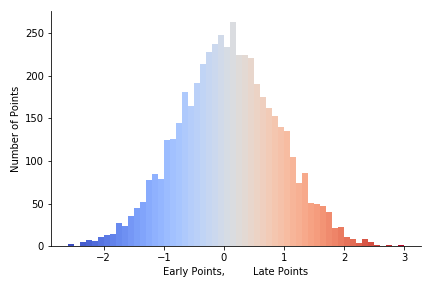
\includegraphics[width=.9\linewidth]{histo5001.png}
    \caption{Number of early and late points of an 
      IDLA cluster at time 5000 
      (same realization and color scale as in 
      Figure \ref{F: IDLA 5000}).}
    \label{F: histo IDLA 5000}
  \end{figure}
\end{remark}

\section{Detect Early and Late Points} 
\label{sec: detect early and late points}
In this section we prove Lemma \ref{No Very Late Point},
\ref{Early Points Imply Late Points}, and 
\ref{Late Points Imply Early Points}, 
which were the core lemmas of the 
proof of Theorem \ref{log fluctuation}.
In order to detect early and late points, we will analyse 
the behavior of $M^{\zeta}$ and its quadratic variation 
on different events.
  

\subsection{Quadratic Variation Bounds}
\label{sec: QV Bounds}
To prove Lemma \ref{Early Points Imply Late Points} 
and \ref{Late Points Imply Early Points} 
we will state two lemmas, which 
bring the martingale from Section \ref{sec: define the martingale} into play. 
Both lemmas show that the absence of early points 
indicates a small quadratic variation $\langle M^{\zeta} \rangle$.\\~\\
For time $t \geq 0$ define the radius
\begin{equation}\label{D: r_0}
  r_0 :=  \sqrt{t/\pi}+4m+2C_1,
\end{equation}
where $C_1$ is defined in Lemma \ref{Properties of H}.
For $|\zeta| > r_0$ and on the event $\mathcal{E}^m(t)^c$ 
the cluster $A^{\zeta}(t)$ is inside $\OZ$. 
In this case, we get the following bound for 
the quadratic variation $ \langle M^{\zeta} \rangle _t$.

\begin{lemma}[No early point implies small quadratic variation]
  \label{no early points then smal QV}
  For each time $t \in \mathbb{N}$ and $\zeta \in \mathbb{Z}^2$ with $| \zeta | \geq r_0$, it is
  $$
    \mathbb{P} \big( \mathcal{E}^{m+1} (t)^c \cap 
    \{ \langle M^{\zeta} \rangle _t > s \} \big)
    \leq t^{80} e^{-s},
  $$
  for $s>0$.
\end{lemma}

For $\zeta$ closer to the origin particles of $A^{\zeta}(t)$ 
may accumulate at $\partial \OZ$, which may yield to a larger 
quadratic variation of $M^{\zeta}(t)$.

\begin{lemma}[No early point implies small quadratic variation 2]
  \label{No early point then small QV 2}
  Fix \hbox{$m \geq 2C_1 + 2$, $l \leq m$}, 
  and $\zeta \in \mathbb{Z}^2$ with $|\zeta| \geq l$. 
  Let $t = \pi (|\zeta| + l)^2$, then 
  $$
    \mathbb{P} \big( \mathcal{E}^{m} (t)^c \cap 
    \{ \langle M^{\zeta} \rangle _t > s \} \big)
    \leq t^{80} e^{1260m} e^{- s},
  $$
  for $s > 0$. 
\end{lemma}

In the proof of Lemma \ref{Early Points Imply Late Points}
we will choose $\zeta$ outside $B_{r_0}$ (and 
Lemma \ref{no early points then smal QV} applies), 
whereas in Lemma \ref{Late Points Imply Early Points} 
we choose $\zeta$ smaller than $\sqrt{t/\pi} - l$ 
(where Lemma \ref{No early point then small QV 2} applies).
Lemma \ref{no early points then smal QV} and \ref{No early point then small QV 2} 
will be proven in Section \ref{sec: Proof QV Bounds}.

\subsection{No Thin Tentacles}
\label{sec: no thin tentacles}
We set
\begin{equation}\label{D: mathbbB(z,r)}
  \nonumber
  \mathbb{B}(z, r) = B(z, r) \cap \mathbb{Z}^2.   
\end{equation}
The next lemma states that if $z \in A(n)$, then the IDLA 
cluster $A(n)$ occupies more then a 
constant fraction of points in the ball $\mathbb{B}(z,m)$ with high probability.  
It is used in Lemma \ref{Early Points Imply Late Points} 
to bound the probability of the event that 
a point $z \in \mathbb{Z}^2$ is $m$-early, but there are just a few 
points in $\mathbb{B}(z,m)$ part of the IDLA cluster (see Figure \ref{F: thin tentacle} below). 
\begin{figure}[H]
  \captionsetup{width=.9\linewidth}
  \centering
  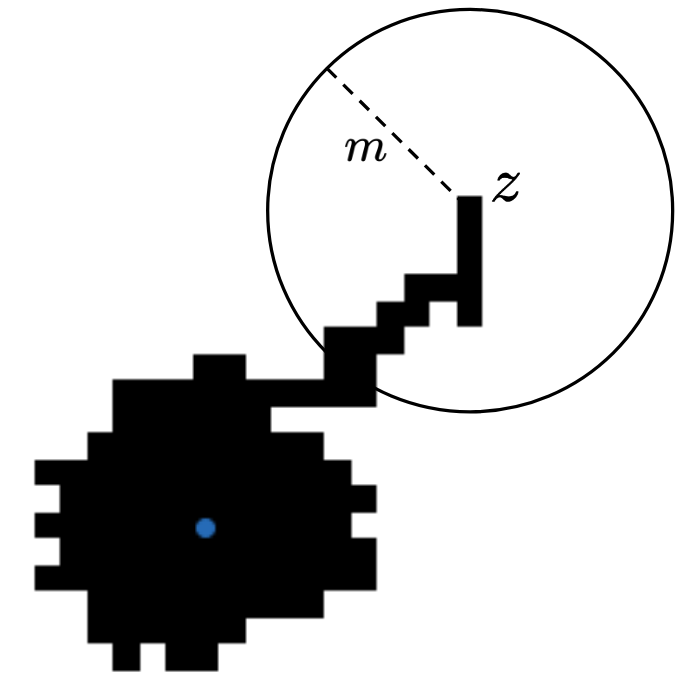
\includegraphics[width=6cm, height=6cm]{thin_tentacle115.png}
  \caption{A thin tentacle of an IDLA cluster by time 119.}
  \label{F: thin tentacle}
\end{figure}
\begin{lemma}[No thin tentacles]
  \label{No Thin Tentacles}
  There are constants $b$, $C_2$, $c_2 > 0$
  such that for all $m>0$ and 
  $z \in \mathbb{Z}^2$ with $0 \notin \mathbb{B}(z,m)$, 
  \begin{equation}\nonumber
    \mathbb{P}\big( z \in A(n),\; 
    | A(n) \cap \mathbb{B}(z,m) | \leq b m ^2  \big) 
    \leq C_2 e^{-c_2 m}.
  \end{equation}  
\end{lemma}

For the proof, I refer to Jerison, Levine, and Sheffield
who proved a similar result for higher dimensions as well 
(see \cite{jerison}, Lemma A).


\subsection{Proof: Early Points Imply Late Points}
\label{sec: detect early points}
We will prove Lemma \ref{Early Points Imply Late Points} 
in this section. The main effort will be dedicated to bound 
$\langle M^{\zeta} \rangle_t$ and $M^{\zeta}(t)$ on events which 
partition $\mathcal{E}^m(t) \cap \mathcal{L}^l(t)^c$.

\begin{proof}[Proof of Lemma \ref{Early Points Imply Late Points}]
  \renewcommand{\qedsymbol}{}
  Since $\mathcal{L}^{l+1}(T) \subset \mathcal{L}^{l}(T)$,
  it suffices to prove the lemma for \mbox{$l=b m /1000$}. 
  If $m > T - \sqrt{T/ \pi}$, then 
  $\mathcal{E}^m(T) = \emptyset$. 
  Hence, we may assume that $m \leq T - \sqrt{T/ \pi}$.
  For each $z \in \mathbb{Z}^2$ and each
  integer $t \in 1,...,T$ define the event that $z$ is the first 
  $m$-early point and joins the IDLA cluster at time $t$ by
  $$
  Q_{z,t} = \{ z \in A(t) \setminus A(t-1) \} \cap
            E^m_z \cap
            \mathcal{E}^m(t-1)^c.
  $$
  If there is at least one $m$-early point up to time $T$,
  then one point in $\mathbb{B}_T$ needs to be the first 
  $m$-early point. This enables us to write 
  $\mathcal{E}^m(T)$ 
  as a disjoint union of the events $Q_{z,t}$,
  \begin{equation}
    \label{eq: partition Em}
    \mathcal{E}^m(T) =
    \bigcup_{t \leq T} \bigcup_{z \in \mathbb{B}_T} Q_{z,t}.
  \end{equation}
  On the event $Q_{z,t}$ it is clear that 
  $A(t) \setminus \{z\} \subset \mathbb{B}_{\sqrt{t/\pi} + m}$
  and also that $z$ cannot be $(m+1)$-early
  (since otherwise a neighbor of $z$ would be $m$-early at time $t-1$).
  Hence, and since $z$ is the first $m$-early point, it is 
  $A(n) \subset \mathbb{B}_{\sqrt{n/\pi}+m+1}$ for all $n \leq t$, 
  and by \eqref{eq: early points as a union},
  \begin{equation}
    \label{eq: Q subset E_m}
      Q_{z,t} \subset \mathcal{E}^{m+1}(t)^c
  \end{equation}
  holds for each $t \in 1,...,T$ and $z \in \mathbb{B}_T$. 
  Fix the time $t \in 1,...,T$ and a point $z \in \mathbb{B}_t$.
  Recall \eqref{D: r_0}, the definition of $r_0 = r_0(t,m)$.
  In order to apply Lemma \ref{no early points then smal QV}, 
  we choose for each $Q_{z,t}$ a $\zeta$ with distance to the origin larger than $r_0$, 
  but close enough to the fixed $z$ such that we can find a 
  sufficient large lower bound of $H^{\zeta}$
  for points close to $z$. Therefore, 
  consider the unit square with lattice point corners containing 
  $r_0 \frac{z}{|z|}$, and define $\zeta = \zeta(z,t,m)$ to 
  be the corner of the square that is farthest from the origin. Then,
  $$
  r_0 \leq |\zeta| \leq r_0 + \sqrt{2}.
  $$
  Choose $s= (2 \gamma + 100) \ln T$.
  So Lemma \ref{no early points then smal QV} leads to 
  \begin{equation} \label{eq: bound QV on Q}
    \begin{split}
      \mathbb{P}(Q_{z,t} \cap 
      \{ \langle M^{\zeta} \rangle _t > s \} )
      &\leq 
      \mathbb{P}(\mathcal{E}^{m+1} (t)^c \cap 
      \{ \langle M^{\zeta} \rangle _t > s \} )\\
      &\leq T^{-(2\gamma + 20)}. 
    \end{split}
  \end{equation}
  In words, on the event $Q_{z,t}$ it is unlikely that 
  the quadratic variation of $\MZT$ is bigger than $\ln (T)$.
  On the other hand, on the event $Q_{z,t} \cap \LLT^c$ it is likely that the martingale
  $\MZT$ is large; more precisely, we will show later that
  \begin{equation}
    \label{eq: bound M on Q}
    \mathbb{P} \big(
      Q_{z,t} \cap \LLT^c \cap \{ \MZT < m (b/25)\}
    \big) 
    < T^{-(\gamma + 5)}. 
  \end{equation}
  However, by Corollary \ref{Small QV implies small martingale} 
  it is unlikely that the quadratic variation is small while the martingale 
  itself is large. Hence, 
  \begin{equation}\label{eq:bound M ad QV M}
    \begin{split}
      \mathbb{P} \big(
        \langle M^{\zeta} \rangle _t \leq s 
        , \; \MZT \geq m \, b/25 
      \big) 
      & \leq 
      \mathbb{P} \big(
        \langle M^{\zeta} \rangle _t \leq s , \; \MZT \geq s 
        \big) \\
      & \leq e^{-s/2} < T^{-(\gamma + 5)},
    \end{split}
  \end{equation}
  where we also used that $m \,b/25 \geq (b/25) C_3 \ln T \geq s$. 
  In conclusion, on the event  
  $Q_{z,t} \cap \LLT^c$ the quadratic variation is likely to be small (see 
  \eqref{eq: bound QV on Q}), and the martingale itself
  is likely to be large (see \eqref{eq: bound M on Q}). 
  However, by \eqref{eq:bound M ad QV M} it is 
  unlikely that the martingale is large while 
  its quadratic variation is small. 
  In keeping with this idea we get
  \begin{equation}\label{eq: Q cap L leq}
    \begin{split}
        \mathbb{P}\big(Q_{z,t} \cap \LLT^c \big) 
      & \leq \mathbb{P} \big(
        Q_{z,t} \cap 
          \{ \langle M^{\zeta} \rangle _t > s \} \big) \\
      & \qquad + \mathbb{P} \big( 
        Q_{z,t} \cap \LLT^c \cap \{ \MZT < m \,b/25 \}\big)\\
      & \qquad + \mathbb{P} \big(
        \langle M^{\zeta} \rangle _t \leq s , \; 
        \MZT \geq m \, b/25 \big) \\
      & \leq 3 T^{-(\gamma + 5)}.
    \end{split}
  \end{equation}
  By summing over all $Q_{z,t}$ (and since $T > 6\pi$), 
  it follows immediately with \eqref{eq: partition Em} that
  \begin{align*}
    \mathbb{P}( \EMT \cap \LLT^c) 
    & = \sum_{t=1}^T \sum_{z \in \mathbb{B}_T} 
          \mathbb{P} \big( Q_{z,t} \cap \LLT^c \big)\\
    & \leq T \cdot (2\pi T^2) \cdot 3T^{-(\gamma + 5)}\\
    & \leq T^{-(\gamma + 1)}.
  \end{align*} 

  It only remains to prove \eqref{eq: bound M on Q}. 
  On the event $Q_{z,t}$, it is
  \begin{equation}\label{eq: A in Oz}
    A(t)  \subset \mathbb{B}_{\sqrt{t /\pi}+ m+ 1} 
          \subset \mathbb{B}_{r_0 - C_1}
          \subset \OZ.
  \end{equation}
  The first inclusion above holds by Equation \eqref{eq: Q subset E_m}, 
  for the second use the definition of \hbox{$r_0$} (see \eqref{D: r_0}), 
  and the third we get from Lemma \ref{Properties of H} (d) and since $|\zeta|$ 
  is nearly $r_0$.  
  Consequently, $\AZT$ consists of lattice points and no particle 
  (grid Brownian motions) of $\AZT$ has been stopped because of reaching 
  the boundary of $\OZ$, which gives
  $$
    \AZT = A(t),
  $$
  on the event $Q_{z,t}$. 

  In order to bound $\MZT$ on the event
  $Q_{z,t} \cap \LLT^c$, partition $\AZT$ into the sets
  $$
    A^1 = \AZT \cap \mathbb{B}_{\sqrt{t/\pi} - l}, \quad
    A^2 = \AZT \cap \mathbb{B}(z, m), \quad 
    A^3 = \AZT \setminus (A^1 \cup A^2),
  $$ 
  as illustrated in Figure \ref{F: IDLA cluster on event} below.
  \begin{figure}[H]
    \captionsetup{width=.9\linewidth}
    \centering
    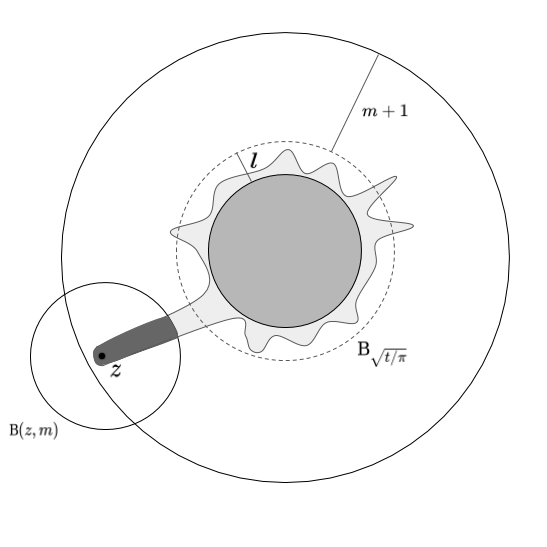
\includegraphics[width=9cm, height=9cm]{Lemma12(3).png}
    \vspace*{-5mm}
    \caption{IDLA cluster at time $t$ on the event 
      $Q_{z,t} \cap \LLT^c$. The cluster is partitioned into 
      $A^1$ (gray), $A^2$ (dark gray), and $A^3$ (light gray).}
    \label{F: IDLA cluster on event}
  \end{figure}
  For each such set, bound its contribution to $\MZT$ from below.
  More precisely, consider the event $W := \{|A^2| > bm^2 \} \cap Q_{z,t} \cap \LLT^c$ and 
  find a sufficiently large lower bound of $\MZT$ on this event. 
  As a consequence, if $\MZT$ is lower than that bound, 
  then $|A^2| \leq bm^2$, which is unlikely to occur by 
  Lemma \ref{No Thin Tentacles} (No thin tentacles). 
  We will give a more thorough explanation in \eqref{eq: M^zeta superset of} and 
  the subsequent inclusions.
  
  Start with $\boldsymbol{A^3}$\textbf{'s contribution} to $\MZT$, 
  which is small since on the event $W$ the fraction 
  $A^3$ cannot contain many points. On the event $\LLT^c$ it is 
  $\mathbb{B}_{\sqrt{t/\pi} - l} \subset \AZT$, hence
  $$
  A^1 = \mathbb{B}_{\sqrt{t/\pi} - l},
  $$
  i.e., most of the particles of $\AZT$ are contained in $A^1$. 
  Hence, the number of particles in $A^2$ or $A^3$ can be bounded by
  \begin{align*}
    |A^2 \cup A^3| 
      = |\AZT| - |A^1| 
      \leq t - \pi(\sqrt{t/ \pi} - l - 1)^2 
      \leq 8 \, l \sqrt{t}.
  \end{align*}
  By Lemma \ref{L: H close to F} we have $H^{\zeta}(0) \leq 2/r_0$. Hence, 
  $$
    \sum_{z \in A^3} \big( H^{\zeta}(z) - H^{\zeta}(0) \big)
    \geq -|A^3| \cdot H^{\zeta}(0) 
    \geq - 8 \, l \sqrt{t} \cdot \frac{2}{r_0}
      \geq - 30 \, l
      \geq -\frac{b}{30} m,
  $$
  where for the first inequality we have used that by $\OZ$'s definition
  $H^{\zeta}$ is positive on $\OZ$. 

  The \textbf{contribution of} $\boldsymbol{A^1}$ is small, since 
  the approximate mean-value property of 
  $H^{\zeta}$ (see Lemma \ref{Properties of H} (f)) implies
  $$
    \sum_{z \in A^1} 
      \big( H^{\zeta}(z) - H^{\zeta}(0) \big) 
    \geq -C_1 \ln |\zeta| 
    \geq -C_1 \ln T 
    \geq -\frac{b}{1000}m,
  $$
  where we used the assumption $m \geq C_3 \ln T$ and $C_3 b/1000 \geq C_1$, 
  which holds by the definition of $C_3$.

  On the event $W$ the \textbf{contribution of} $\boldsymbol{A^2}$ is 
  the largest, since the fraction $A^2$ contains at least $bm^2$ points and 
  $H^{\zeta}$ is larger on $A^2$ ($A^2$ is closer to $\zeta$ than $A^1$ and $A^3$).    
  The distance between $z$ and $\zeta$ is (up to a constant) $3m$. 
  In addition, $z$ and $\zeta$ are (nearly) on the 
  same ray through $0$. Therefore, 
  using Lemma \ref{Propeties of F} \ref{p: F is shift of K}, 
  \begin{equation}\nonumber
    F^{\zeta}(z) = 
    \frac{|\zeta| +|z| + |\zeta - z|}
      {2|\zeta| |\zeta - z|} 
    \approx \frac{1}{3m}
  \end{equation} 
  Hence, for $\tilde{z} \in \mathbb{B}(z,m)$ 
  using the estimations Lemma \ref{L: H close to F} and 
  Lemma \ref{Propeties of F} \ref{p: sup of F^zeta on small circles}, we get 
  \begin{equation}\nonumber
  \begin{split}
    H^{\zeta}(\tilde{z}) 
    = H^{\zeta}(\tilde{z}) - F^{\zeta}(\tilde{z})
      + F^{\zeta}(\tilde{z}) - F^{\zeta}(z) 
      + F^{\zeta}(z)
    = O\Big( \frac{1}{m^2} \Big) + \frac{1}{3m}.
  \end{split}
  \end{equation}
  By using Lemma \ref{L: H close to F} once again, 
  it is $H^{\zeta}(0) = 1/r_0 + O(1/r_0^2) \leq 1/4m + O(1/m^2)$, 
  and we obtain 
  $H^{\zeta}(\tilde{z}) - H^{\zeta}(0) \geq  1/12m + O(1/m^2) \geq 1/13 m$. 
  Thus, 
  $$
  \sum_{\tilde{z} \in A^2} 
  \big(H^{\zeta}(\tilde{z}) - 
    H^{\zeta}(0) \big) 
  \geq |A^2| \frac{1}{13m} 
  > bm^2 \frac{1}{13m} 
  = \frac{b}{13} m.
  $$
  Summing over $\boldsymbol{A^1, \, A^2}$, and $\boldsymbol{A^3}$  provides 
  \begin{equation}\nonumber
    \MZT > 
    \Big( \frac{b}{13} - 
    \frac{b}{30} - \frac{b}{1000} \Big) m 
    > \frac{b}{25}m,
  \end{equation}
  on the event $W$. Hence,
  \begin{equation}\label{eq: M^zeta superset of}
    \Big{\{} \MZT > \frac{b}{25}m \Big{\}} \, \supset \, 
    \{|A^2| > bm^2\} \cap Q_{z,t} \cap \LLT^c,
  \end{equation}
  taking the complement, 
  $$
  \Big{\{} \MZT \leq \frac{b}{25}m \Big{\}} 
  \, \subset \,
      \{|A^2| \leq bm^2\} \cup Q_{z,t}^c \cup \LLT,
  $$
  and intersecting with $Q_{z,t} \cap \LLT^c$ gives
  $$
  \Big{\{} \MZT \leq \frac{b}{25}m \Big{\}} 
  \cap Q_{z,t} \cap \LLT^c
  \, \subset \, \{|A^2| \leq bm^2\} \cap Q_{z,t} \cap \LLT^c.
  $$
  However, by Lemma \ref{No Thin Tentacles} it is unlikely 
  that $|A^2| \leq bm^2$, i.e.,
  \begin{align*}
    \mathbb{P} \big( 
      \big{\{} \MZT \leq (b/25)m \big{\}} 
      \cap Q_{z,t} \cap \LLT^c \big) 
    & \leq \mathbb{P} \big(
      \{|A^2| \leq bm^2\} \cap Q_{z,t} \cap \LLT^c
      \big) \\
    & < C_2 e^{-c_2 m} \\
    & < T^{-(\gamma + 5)},
  \end{align*}
  which finishes the proof.
\end{proof}

\subsection{Proof: Late Points Imply Early Points}
\label{sec: detect late points}
In this section we prove Lemma \ref{Late Points Imply Early Points}.
It can be considered as the reverse analog of Lemma 
\ref{Early Points Imply Late Points}, and 
the main tools we will need were already used 
in the proof of Lemma \ref{Early Points Imply Late Points}. 
Similar to the proof of Lemma \ref{Early Points Imply Late Points} we will 
partition $\mathcal{L}^l(T) \cap \mathcal{E}^m(T)^c$ and bound $M^{\zeta}$ 
and its quadratic variation on each set in that partition. 
While for Lemma \ref{Early Points Imply Late Points} 
we chose for certain subevents of $\mathcal{E}^m(T)$ a 
$\zeta$ such that $A^{\zeta}$ is contained inside $\OZ$ (see \eqref{eq: A in Oz}), 
our choice of $\zeta$ will now imply that 
some particles of $A^{\zeta}$ need to accumulate on $\partial \OZ$.

\begin{proof}[Proof of Lemma \ref{Late Points Imply Early Points}]
  Start with the observation that, since $\mathcal{E}^m(T)$ is decreasing in $m$,
  we may assume without a loss 
  of generality  $m = l^2 / (C_4 \ln T)$. 
  Since $l \geq C_4 \ln T$ we have $m \geq l$. 
  Partition $\mathcal{L}^l(T)$ into the events 
  that single points are $l$-late, which we defined in \eqref{D: L_l(T)},
  $$
    \mathcal{L}^l(T) = 
    \bigcup_{\zeta \,:\, 
    |\zeta| \leq \sqrt{T/\pi} - l} L^l_{\zeta}.
  $$
  Now fix a point $\zeta \in \mathbb{B}_{\sqrt{T/\pi} - l}$ 
  that is potentially $l$-late by time $T$. 
  Define the time $T_{\zeta} = \pi(|\zeta| + l)^2$ 
  at which $\zeta$ is not part of the IDLA cluster 
  on the event $L^l_{\zeta}$.

  To bound the probability of the event
  $\mathcal{L}^l(T) \cap \mathcal{E}^m(T)^c$ 
  we consider 
  (similar to Equation \eqref{eq: Q cap L leq} in the proof of 
  Lemma \ref{Early Points Imply Late Points}) 
  $\mathcal{E}^m(T)^c$ on the event $\QV_{T_{\zeta}} > s$ and 
  $L^l_{\zeta}$ on the counter event, i.e.,
  \begin{equation}\label{eq: bound L cap EmT^c}
    \begin{split}
      \mathbb{P}(L^l_{\zeta} \cap \mathcal{E}^m(T)^c) 
      & \leq  \mathbb{P}(\mathcal{E}^m(T)^c \cap \{ \QV_{T_{\zeta}} > s\})\\
          & \;\;\;\;\; +\mathbb{P}(L^l_{\zeta} \cap \{ \QV_{T_{\zeta}} \leq s \} ),
    \end{split}
  \end{equation}
  for an $s$, which we will pick in the next step.

  Consider the first summand on the right side and  
  note that $T_{\zeta} \leq T \leq e^m$. 
  Suppose $|\zeta| \geq l$, which enables us to apply 
  Lemma \ref{No early point then small QV 2}; hence, 
  \begin{equation}\label{eq: bound QV on EmT complement}
    \begin{split}
      \mathbb{P}(\mathcal{E}^m(T)^c \cap \{ \QV_{T_{\zeta}} > s\})
        & \leq  T_{\zeta}^{80} e^{1260m} e^{-s} 
        \leq e^{1340 m - s}\\
        &  \leq e^{-10 m}
        \leq e^{-10 (\gamma + 3) \ln T}\\
        &  \leq T^{-(\gamma + 3)}, 
    \end{split}
  \end{equation}
  where we set $s = 1350 m$. 

  Next bound the second summand of \eqref{eq: bound L cap EmT^c}.
  For this purpose, show that on the event
  $L^l_{\zeta}$ it is $M^{\zeta}(T_{\zeta}) \leq -l$.
  The strategy is to split the sum of $H^{\zeta}(z) - H^{\zeta}(0)$ 
  over all $z \in A^{\zeta}(T_{\zeta})$ into 
  \begin{itemize}
    \item
      the particles on $\partial \OZ \setminus \{\zeta\}$
      (here, $H^{\zeta}(\mydot) - H^{\zeta}(0)$ 
      is small and constant)
    \item
      and the particles in $\OZ$ (here, the sum of 
      $H^{\zeta}(\mydot) - H^{\zeta}(0)$ over all these particles 
      is small by the approximate mean-value property of $H^{\zeta}$ that can be applied if 
      all sites in $\OZ$ are occupied, see Lemma \ref{Properties of H} (f)).  
  \end{itemize}
  On the event $L^l_{\zeta}$ no particle in $A^{\zeta}(T_{\zeta})$ reaches $\zeta$, 
  where $H^{\zeta}$ is much larger than on every other boundary point, 
  where $H^{\zeta}$ equals $\frac{1}{2|\zeta|}$ (see Lemma \ref{Properties of H}). 
  In addition, by the choice of $\zeta$ and $T_{\zeta}$ 
  some particles of $A^{\zeta}(T_{\zeta})$ need to accumulate at $\partial \OZ \setminus \{\zeta\}$.
  More precisely, since $\OZ \subset B_{|\zeta| + C_1}$ (see Lemma \ref{Properties of H} (d)), 
  we have 
  \begin{equation} \nonumber
    T^{\zeta} - |\OZ \cap \mathbb{Z}^2| 
    \geq \pi(|\zeta| + l)^2 - \pi (|\zeta| + C_1 + 1)^2
    \geq \pi |\zeta| l,
  \end{equation}
  i.e, on the event $L^l_{\zeta}$ at least $\pi |\zeta| l$ particles 
  accumulate at $\partial \OZ \setminus \{\zeta\}$. 
  For these particles we have by Lemma \ref{L: H close to F},
  $$
    H^{\zeta}(z)-H^{\zeta}(0) 
    \leq - \frac{1}{2|\zeta|} + O \Big( \frac{1}{|\zeta|^2} \Big).
  $$
  Hence, 
  \begin{equation}\label{eq: sum over A^zeta cap Z}
    \sum_{z \in A^{\zeta}(T_{\zeta}) \cap \partial \OZ}
    \big( H^{\zeta}(z) - H^{\zeta}(0) \big) 
    \leq -\pi |\zeta| l \mydot \frac{1}{2|\zeta|} 
    \leq -\frac{3}{2} l. 
  \end{equation}
  Otherwise, provided the event $L^l_{\zeta}$, our martingale $M^{\zeta}(T_{\zeta})$ 
  is maximized if all sites in $\OZ$ are occupied by $A^{\zeta}(T_{\zeta})$. 
  This results from the definition of $\OZ$, according to which $H^{\zeta}$ achieves 
  its minimum over $\bar{\Omega}_{\zeta}$ in every point on \mbox{$\partial \OZ \setminus \{\zeta\}$}.
  In this case, when all points in $\OZ \cap \mathbb{Z}^2$ are occupied by $A^{\zeta}(T_{\zeta})$, 
  we can use Lemma \ref{Properties of H} (f), which implies 
  \begin{equation}\label{eq: sum over OZ cap Z}
    \sum_{z \in \OZ \cap \mathbb{Z}^2}
    (H^{\zeta}(z) - H^{\zeta}(0))
    \leq C_1 \ln |\zeta| 
    \leq C_1 \ln T 
    \leq \frac{1}{2} l,
  \end{equation}
  where for the last inequality we used $ l \geq C_4 \ln T$ and $C_4 > 2 C_1$.
  The statements \eqref{eq: sum over A^zeta cap Z} and \eqref{eq: sum over OZ cap Z} give us 
  \begin{equation} \nonumber
    \begin{split}
      M^{\zeta}(T_{\zeta})
      & \leq 
        \sum_{z \in A^{\zeta}(T_{\zeta}) \cap \partial \OZ}
        \big( H^{\zeta}(z) - H^{\zeta}(0) \big) + 
        \sum_{z \in \OZ \cap \mathbb{Z}^2}
      \big(H^{\zeta}(z) - H^{\zeta}(0) \big)  \\
      & \leq -l,
    \end{split}
  \end{equation}
  on the event $L^l_{\zeta}$, i.e., 
  $L^l_{\zeta} \subset \{M^{\zeta}(T_{\zeta}) \leq -l \}$;
  and by Corollary \ref{Small QV implies small martingale} 
  it is unlikely that the modulus of the martingale 
  is large while its quadratic variation is small. Thus, 
  \begin{equation}\label{eq: bound QV on L_zeta}
    \begin{split}
        \mathbb{P} \big(L^l_{\zeta} \cap \{ \QV_{T_{\zeta}} \leq s \} \big)
      & \leq 
      \mathbb{P} \big(\{M^{\zeta}(T_{\zeta}) \leq -l \} \cap \{ \QV_{T_{\zeta}} \leq s \} \big)\\ 
      & \leq e^{-\frac{l^2}{2700m}} \leq T^{-(\gamma + 3)},
    \end{split}
  \end{equation}
  where we used the inequality $l^2/(2700m) > (\gamma + 3) \ln T$, 
  which holds by the assumption on $m$ and since $C_4 \geq 2700(\gamma + 3)$. 

  Combining \eqref{eq: bound L cap EmT^c}, \eqref{eq: bound QV on EmT complement}, 
  and  \eqref{eq: bound QV on L_zeta}, yields 
  $$
    \mathbb{P} \big( L^l_{\zeta} \cap \mathcal{E}^m(T)^c \big)
    \leq 2 T^{-(\gamma + 3)},
  $$ 
  for all $\zeta$ with $l \leq |\zeta| \leq \sqrt{T/\pi} - l$.

  Using Lemma \ref{No Very Late Point}, we can handle all $\zeta$ where $|\zeta| < l$ 
  at once,
  \begin{equation}
    \mathbb{P} \bigg(  
      \bigcup_ {\zeta \,:\, |\zeta| < l} L^l_{\zeta} \bigg)
    = \mathbb{P} \big( \mathcal{L}^l(4\pi l^2) \big) 
    \leq C_2 e^{-c_2 l} < T^{-(\gamma+3)}. \nonumber
  \end{equation} 
  In total,
  \begin{equation}\nonumber
    \begin{split}
      \mathbb{P}(\mathcal{L}^l(T) \cap \mathcal{E}^m(T)^c) 
      & \leq 
        \mathbb{P}\Bigg(\bigcup_ {|\zeta| < l}
        L^l_{\zeta} \cap \mathcal{E}^m(T)^c \Bigg)
      + \mathbb{P}\Bigg( \bigcup_{l \leq |\zeta| < \sqrt{T/\pi}-l} 
      L^l_{\zeta} \cap \mathcal{E}^m(T)^c \Bigg)\\
      & \leq T^{-(\gamma + 3)} + T\cdot 2 T^{-(\gamma + 3)} \\
      &  \leq T^{-(\gamma+1)}. 
    \end{split}
  \end{equation}
\end{proof}


\subsection{Proof: Quadratic Variation Bounds}
\label{sec: Proof QV Bounds}
Here we prove Lemma \ref{no early points then smal QV} and \ref{No early point then small QV 2}, 
which bound $\langle M^{\zeta}\rangle$ on the event of no $m$-early point.
We first state Lemma \ref{small increment of QVM}, which bounds 
increments of $\langle M^{\zeta}\rangle$ of size one by exit times of Brownian motions. 
In both proofs of Lemma \ref{no early points then smal QV} and 
\ref{No early point then small QV 2} we will split 
$\langle M^{\zeta}\rangle$ into increments of size one, apply Lemma \ref{small increment of QVM}, 
and then use Lemma \ref{exit times of BM} to bound the exit times. 
\\~\\ 
For $A \subset \mathcal{G}$ define 
$$
  \tilde{A} = \OZ \cap 
  \bigcup_{z \in A \cap \mathbb{Z}^2} (z + E),
$$
where $E \subset \mathcal{G}$ denotes the open cross, 
defined in Section \ref{sec: stoch analysis on the grid}.
With the notation of Lemma \ref{L: M as BM}, let 
$\tilde{\mathcal{B}}^n(u) := 
  \mathcal{B}(\langle M^{\zeta} \rangle_n + u)
  - \mathcal{B} (\langle M^{\zeta} \rangle _n)$, 
which is, since $\langle M^{\zeta} \rangle_n$ is an $\mathcal{F}_{T_s}$-stopping time, 
a Brownian motion (see for instance \cite{revuz}, Ch. III, Cor. 3.6).
Denote the exit times
\begin{equation}\nonumber
  \tau_{(-a_n, b_n)}^n = 
  \inf \{ u \geq 0 \,|\, 
    \tilde{\mathcal{B}}^n(u) 
    \notin [-a_n, b_n] \}.
\end{equation}

\begin{lemma}
  \label{small increment of QVM}
  Fix $\zeta \in \mathbb{Z}^2$. 
  For $n \in \mathbb{N}$ let 
  \begin{equation}  \nonumber
    \begin{split}
      - & a_n = \min \big{\{}
        H^{\zeta}(z) - H^{\zeta}(0) \,\big|\, 
        z \in \partial \tilde{A}^{\zeta}(n) \big{\}},\\
      & b_n = \max
      \big{\{} H^{\zeta}(z) - H^{\zeta}(0) \, \big|\, 
      z \in \partial \tilde{A}^{\zeta}(n) \big{\}},
    \end{split}
  \end{equation}
  then we have
  $$
    \langle M^{\zeta} \rangle _{n+s} - 
    \langle M^{\zeta} \rangle _n
    \leq \tau_{(-a_n, b_n)}^n,
  $$
  for all $s \in [0,1]$.
\end{lemma}

\begin{proof}
  $H^{\zeta}$ is grid-harmonic on $\tilde{A}^{\zeta}(n) \subset \OZ$  
  (see Lemma \ref{Properties of H} (c)).
  By applying maximum principle (Lemma \ref{L: maximum principle grid}) to 
  $H^{\zeta}(\mydot) - H^{\zeta}(0)$, we get
  $$
    H^{\zeta}(z) - H^{\zeta}(0) \in [-a_n, b_n],
  $$
  for all $z \in \tilde{A}^{\zeta}(n)$. From the definition of $\MZT$ it is 
  $$
    \MZT - M^{\zeta}(n) \in [-a_n, b_n],
  $$
  for all $t \in [n, n+s]$.
  Using Lemma \ref{L: M as BM}, the representation of $M^{\zeta}$ as a Brownian motion, 
  we conclude for 
  $r \in [ \langle M^{\zeta} \rangle _n, \langle M^{\zeta} \rangle _{n+s}]$ that
  $$
    \mathcal{B}(r) - 
    \mathcal{B}( \langle M^{\zeta} \rangle _n)
    \in [-a_n, b_n],
  $$
  which is equivalent to the statement that
  $$
    \tilde{\mathcal{B}}^n(u) = 
    \mathcal{B}(\langle M^{\zeta} \rangle _n + u) 
      - \mathcal{B}(\langle M^{\zeta} \rangle _n)
      \in [-a_n, b_n],
  $$
  for all
  $u \in [0, \langle M^{\zeta} \rangle _{n+s} 
            -\langle M^{\zeta} \rangle _n ]$.
  This result can be rephrased as follows:
  the first exit of $\,\tilde{\mathcal{B}}^n(\mydot)$
  from the interval $[-a_n, b_n]$ cannot occur before time 
  $\langle M^{\zeta} \rangle _{n+s} -\langle M^{\zeta} \rangle _n$,
  which enables us to write,
  $$
  \langle M^{\zeta} \rangle _{n+s} 
    - \langle M^{\zeta} \rangle _n
  \leq \tau_{(-a_n, b_n)}^n
  .$$
\end{proof}

Recall that Lemma \ref{no early points then smal QV} 
assumes $|\zeta| > r_0 = r_0(t,m)$ for $r_0$ defined as in \eqref{D: r_0}. 
In this case, we have good bounds for $-a_n$ and $b_n$ on the event $\mathcal{E}^{m+1}(t)^c$, 
for $-a_n$, $b_n$ as defined in Lemma \ref{small increment of QVM}.
 
\begin{proof}[Proof of Lemma \ref{no early points then smal QV}]
  Fix time $t > 0$.
  The event $\mathcal{E}^{m+1} (t)^c$ is equal to the event that 
  \begin{equation*}
    A(n) \subseteq \mathbb{B}_{\sqrt{n/ \pi} + m + 1},\;\;\;
    \text{for all}\; n= 1,...,t.
  \end{equation*}
  Lemma \ref{Properties of H} (d) gives us
  $\mathbb{B}_{\sqrt{n/ \pi} + m + 1} \subset \OZ$, 
  which implies that in the event $\mathcal{E}^{m+1} (t)^c$, it is
  $$
    A^{\zeta}(n) = A(n)
  $$
  We now apply Lemma \ref{Properties of H} (e)
  with the radius  $\sqrt{n/\pi} + m +2 < |\zeta| - C_1$,
  and get the bounds
  $$
    -a := - \frac{1}{2r_0} \leq
    H_{\zeta}(z) - H_{\zeta}(0) \leq
    \frac{1}{r_0 - \sqrt{n/\pi} - m -2 - C_1}
    =: b_n,
  $$
  for all integers $n \leq t$ and $z \in A^{\zeta}(n)$ 
  on the event $\mathcal{E}^{m+1} (t)^c$.
  Hence, on $\mathcal{E}^{m+1} (t)^c$ Lemma \ref{small increment of QVM} 
  implies (with $s=1$) that
  $$
    \langle M^{\zeta} \rangle _{n+1} 
    - \langle M^{\zeta} \rangle _{n}
    \leq \tau_{(-a, b_n)}^n,
  $$
  where $\tau^n_{(-a, b_n)}$ are independent exit times of 
  standard Brownian motions starting at zero. 
  Summing over all increments of size one,
  \begin{equation}\nonumber
    \begin{split}
      \exp (\langle M^{\zeta} \rangle _t) 
      \boldsymbol{1}_{\mathcal{E}^{m+1}(t)^c}
      & \leq 
      \exp \big( 
        \langle M^{\zeta} \rangle _t \, \boldsymbol{1}_{\mathcal{E}^{m+1}(t)^c}
        \big)\\
      & = \exp \Big(
            \sum_{n=1}^{t}
                (\langle M^{\zeta} \rangle _{n} - 
                  \langle M^{\zeta} \rangle_{n-1}) \,
            \boldsymbol{1}_{\mathcal{E}^{m+1}(t)^c} \Big)\\
      & \leq \exp \Big(
        \sum_{n=1}^{t} \tau^n_{(-a, b_n)} \Big).
    \end{split}
  \end{equation}
  To bound the exit times $\tau^n_{(-a, b_n)}$
  observe that for the interval $(-a, b_n)$ and 
  $\lambda = 1$ the assumptions of Lemma \ref{exit times of BM}
  are fulfilled, and since the exit times are independent
  \begin{equation} \nonumber
    \begin{split}
      \Ex \bigg( \exp \Big( \sum_{n=1}^{t} \tau^n_{(-a, b_n)} \Big) \bigg)
      & = \prod_{n=1}^{t} \Ex \big( \exp ( \tau^n_{(-a, b_n)}) \big)
        \leq \prod_{n=1}^{t} (1 + 20ab_n) \\
      & = \exp \; \ln \; \prod_{n=1}^{t} (1 + 20ab_n)
        = \exp \; \sum_{n=1}^{t} \ln(1 + 20ab_n)\\
      & \leq \exp \Big( 20a \sum_{n=1}^{t} b_n \Big).
    \end{split}
  \end{equation} 
  To find a more handy bound denote 
  $R = r_0 - m - 3 - C_1$. Using 
  $$
    b_n = \frac{1}{R + 1 - \sqrt{n / \pi}}  
        \leq \frac{1}{R - \sqrt{(n-1) / \pi}},
  $$
  we can dominate $b_n$, $n = 1,...,t$ and get
  \begin{equation} \nonumber
    \begin{split}
      \sum_{n=1}^{t} b_n 
      & = \sum_{n=1}^{t} 
          \frac{1}{R + 1 - \sqrt{n / \pi}} \\
      & \leq \int_0^{t} 
        \frac{dx}{R  - \sqrt{x / \pi}} \\
      & \leq 2 \pi \int_0^{\sqrt{t/ \pi}} 
        \frac{ y \, dy}{R  - y} \\
      & \leq 2\pi 
          \int_{R- \sqrt{t / \pi}}^R
            \frac{R-z}{z} dz\\
      & = 2\pi R \bigg(
        \ln \bigg( \frac{R}{R-\sqrt{t / \pi}} \bigg)
          - \sqrt{t / \pi} \bigg)\\
      & \leq 2\pi r_0 \ln(r_0 /C_1).
    \end{split}
  \end{equation}
  Together with the Markov inequality, 
  \begin{equation}\label{eq: last step of bound QV 1}
    \begin{split}
      \mathbb{P}(\mathcal{E}^{m+1} (t)^c \cap 
          \{ \langle M^{\zeta} \rangle _t > s \} )
      & \leq \frac{1}{e^s} 
            \Ex \big( \exp (\langle M^{\zeta} \rangle _t) 
                \, \boldsymbol{1}_{\mathcal{E}^{m+1} (t)^c} 
            \big)\\
      & \leq \frac{1}{e^s} 
        \Ex \bigg( \exp 
          \sum_{n=1}^{t} \tau^n_{(-a, b_n)} \bigg) \\
      & \leq
          \frac{1}{e^s} 
            \exp \Big( 20a \sum_{n=1}^{t} b_n \Big) \\
      & \leq \frac{1}{e^s}
        \exp (40a\pi r_0 \ln(r_0 / C_1)) \\
      & \leq \frac{1}{e^s} \bigg( \frac{r_0}{C_1} \bigg)^{20 \pi} 
      \leq \frac{1}{e^s} t^{80}.
    \end{split}
  \end{equation}
\end{proof}

In the last proof, on the event of no $m$-early point the grid IDLA $A^{\zeta}(t)$ 
stayed inside balls, which are subsets of $\OZ$ and keep some distance to $\OZ$. 
Hence, Lemma \ref{Properties of H} (e) provides a good bound on 
$H^{\zeta}(z)- H^{\zeta}(0)$ for all $z$ in $A^{\zeta}(t)$. 
In Lemma \ref{No early point then small QV 2} $\zeta$ may be chosen much smaller
than in Lemma \ref{no early points then smal QV}. 
It follows that particles of $A^{\zeta}(t)$ may accumulate at $\partial \OZ$; 
in particular, they might hit $\zeta$.
For these particles, we will need different bounds of $H^{\zeta}(\mydot) - H^{\zeta}(0)$, 
see \eqref{eq: rough bound on H}. 
Since this bound is too rough to apply it to all particles of $A^{\zeta}(t)$, 
we will pick some time $t_0$ before $t$ such that $A^{\zeta}(t_0)$ is inside 
$\mathbb{B}_{|\zeta|-C_1}$; for the cluster $A^{\zeta}(t_0)$ we can apply 
Lemma \ref{no early points then smal QV}.

\begin{proof}[Proof of Lemma \ref{No early point then small QV 2}]
  First consider the case $|\zeta| \geq 5m$.  
  Choose $t_0$ so that $r_0(t_0)$ is just a little smaller than $|\zeta|$,  
  here,  \mbox{$t_0 = \pi (|\zeta| - 4m - 2C_1 - 1)^2$}. 
  By $t_0, ..., t_N$ denote the sequence
  $t_0,\, \lceil t_0 \rceil,\, \lceil t_0 \rceil +1,\,...,\, \lfloor t \rfloor, \, t$. 
  To bound $\Ex ( e^{\QVT} \, \boldsymbol{1}_{\mathcal{E}^m(t)^c})$ 
  consider separately the increment of 
  $\QV_{\bullet}$ up to time $t_0$ and the increments over 
  the intervals $[t_0, t_1], ..., [t_{N-1}, t_N]$, i.e., write
  \begin{equation}\label{eq: split into incements}
    \begin{split}
      e^{\QVT} \, \boldsymbol{1}_{\mathcal{E}^m(t)^c}
      & \leq  e^{\QVT}  \boldsymbol{1}_{\mathcal{E}^m(t_0)^c} \\
      & = e^{\QV_{t_0}}  \boldsymbol{1}_{\mathcal{E}^m(t_0)^c} 
        \prod_{n=1}^N e^{\QV_{t_n} - \QV_{t_{n-1}}}.
    \end{split}
  \end{equation}
  Lemma \ref{Properties of H} (a) and (e) provide the estimations,  
  \begin{equation}\label{eq: rough bound on H}
      -a := - \frac{1}{2|\zeta|} \leq H^{\zeta}(z) - H^{\zeta}(0) \leq 2 =: b,
  \end{equation}  
  which hold on the entire set $\bar{\Omega}_{\zeta}$. 
  Hence, Lemma \ref{small increment of QVM} implies
  $$
    \QV_{t_n} - \QV_{t_{n-1}} \leq \tau^{t_n}_{(-a, b)},
  $$
  for all $n = 1,...,N$. 
  Moreover, since the Brownian motions $\tilde{\mathcal{B}}^{t_n}(\mydot)$ are independent of 
  each other, of $\mathcal{F}_{t_0}$, and therefore of 
  $\mathcal{E}^m(t_0)^c \in \mathcal{F}_{t_0}$ as well, 
  the same holds for the exit times $\tau^{t_n}_{(-a, b)}$. 
  Applying all this to \eqref{eq: split into incements}, yields 
  \begin{equation}\label{eq: since independent}
    \begin{split}
      \Ex \big( e^{\QVT} \, \boldsymbol{1}_{\mathcal{E}^m(t)^c} \big)
      &\leq \Ex \bigg( e^{\QV_{t_0}}  \boldsymbol{1}_{\mathcal{E}^m(t_0)^c}  
        \prod_{n=1}^N  e^ {\tau^{t_n}_{(-a,b)}}  \bigg)\\
      &= \Ex \big( e^{\QV_{t_0}}  \boldsymbol{1}_{\mathcal{E}^m(t_0)^c} \big)
          \prod_{n=1}^N \Ex \big( e^{\tau^{t_n}_{(-a,b)}}  \big) 
    \end{split}
  \end{equation}

  For the product of the expected exit times in \eqref{eq: since independent}, 
  Lemma \ref{exit times of BM} gives us
  \begin{equation} \label{eq: bound later incements}
    \begin{split}
      \prod_{n=1}^N  \Ex \Big( e^{\tau^{t_n}_{(-a,b)}} \Big)
      & \leq \exp  \ln  \prod_{n=1}^N \frac{20}{|\zeta|} \\
      & \leq \exp \sum_{n=1}^N \frac{20}{|\zeta|} \\
      & \leq \exp \bigg( (t-t_0 +2) \frac{20}{|\zeta|} \bigg) \\
      & \leq \exp (960 m),
    \end{split}
  \end{equation}
  where for the last inequality we used that $t_0$ and $t = \pi(|\zeta| +l)^2$ 
  are not all that far from each other (use also $|\zeta| \geq 5m$ and $m \geq 2C_1 + 2$).

  To bound the factor $\Ex (e^{\QV_{t_0}}  \boldsymbol{1}_{\mathcal{E}^m(t_0)^c})$ 
  in \eqref{eq: since independent}, note that since \hbox{$r(t_0) < |\zeta|$}, 
  the assumptions of Lemma \ref{no early points then smal QV} are fulfilled, 
  thus, by \eqref{eq: last step of bound QV 1},
  \begin{equation}\label{eq: bound incement up to t0}
    \Ex \big( e^{\QV_{t_0}} \, \boldsymbol{1}_{\mathcal{E}^m(t_0)^c} \big)
    \leq t_0^{80} \leq t^{80}.
  \end{equation}

  Plugging \eqref{eq: bound later incements} and \eqref{eq: bound incement up to t0}  
  into \eqref{eq: since independent}, gives us
  \begin{equation}\label{eq: first}
     \Ex \big( e^{\QV_{t}} \,  \boldsymbol{1}_{\mathcal{E}^m(t)^c} \big)
        \leq t^{80} e^{960m},
  \end{equation}

  For the case $|\zeta| \leq 5m$, use the equations 
  \eqref{eq: bound later incements} and \eqref{eq: since independent} with $t_0 = 0$. Then,
  \begin{equation}\label{eq: sec}
    \begin{split}
      \Ex \big( e^{\QV_{t}} \,  \boldsymbol{1}_{\mathcal{E}^m(t)^c} \big)
      &\leq \exp\Big( (t+2)\frac{20}{|\zeta|} \Big)
      \leq \exp \Big( 80\pi|\zeta| + \frac{40}{|\zeta|} \Big)\\
      &\leq \exp (1260m)
    \end{split}
  \end{equation}

  Using Markov inequality, \eqref{eq: first}, and \eqref{eq: sec},
  \begin{equation*}
    \mathbb{P}(\mathcal{E}^{m} (t) ^c \cap \{ \langle M^{\zeta} \rangle _t > s \})
      \leq \Ex \big( e^{\QV_{t}} \, 
      \boldsymbol{1}_{\mathcal{E}^m(t)^c} \big)\, e^{-s}
        \leq t^{80} e^{1260m} e^{-s}. 
  \end{equation*}
\end{proof}

\subsection{Proof: No Very Late Point}
\label{sec: no very late point}
We now present the proof of Lemma \ref{No Very Late Point}. 
It is basically a reformulation of \cite{lawler_idla} Lemma 6 
in terms of late points. 

\begin{proof}[Proof of Lemma \ref{No Very Late Point}]
  \renewcommand{\qedsymbol}{}
  Rephrasing the first conclusion of \cite{lawler_idla} 
  Lemma 6, for each $\epsilon > 0$ and $r$ sufficiently large, it is 
  \begin{equation} \label{eq: Lawler very late points}
    \mathbb{P} \Big( z \notin A 
    \big( \pi \big( r\sqrt{1+ \epsilon} \big) ^2 \big) \Big)
    \leq e^{-c r}, 
  \end{equation}
  for each $z \in \mathbb{B}_{r (1-\epsilon)}$ and a 
  constant $c>0$ that only depends on $\epsilon$.
  In terms of late points, \eqref{eq: Lawler very late points} means that we have an 
  exponential bound for $l$-late points if $l$ is proportional to $r$, where $r$ 
  is the radius of the ball, which describes the expected shape of the 
  cluster by time $T = \pi r^2$.

  Fix $l \geq 1$. It suffices to prove the lemma for 
  $T=100\pi l^2$, and since 
  \begin{equation}\label{eq: parttition very late poits}
      \mathcal{L}^l(100\pi l) 
    = \bigcup_{z \in \mathbb{B}_{9l}}  
      \big{\{} z \notin A 
        \big( \pi ( |z| + l ) ^2 \big) \big{\}},
  \end{equation}
  we may assume $|z| \leq 9l$.
  To apply \eqref{eq: Lawler very late points} to the event of $z$ being $l$-late,
  find $\epsilon$ and $r$ such that
  \begin{equation}\label{eq: epsilon r}
    \begin{split}
      & r (1-\epsilon) > |z|, \;\;\; \text{and}\\
      & r \sqrt{1+ \epsilon} < |z| + l. 
    \end{split}
  \end{equation}
  The first inequality ensures that $z \in \mathbb{B}_{r (1-\epsilon)}$. 
  Together with \eqref{eq: Lawler very late points} 
  we obtain from the second inequality
  \begin{equation} \nonumber
    \mathbb{P} \big( z \notin A 
      \big( \pi ( |z| + l ) ^2 \big) \big)
      \leq e^{-c r}. 
  \end{equation}
  Assume that $r$ is of the form 
  $r = a(\epsilon)(|z| + l)$, 
  for some $a$ just depending on $\epsilon$.
  Such an $r$, which 
  fulfills the inequalities of \eqref{eq: epsilon r}, 
  exists if there is an $a=a(\epsilon)$, which fulfills
  $$
    \frac{9}{10} \frac{1}{1-\epsilon}
    < a < \frac{1}{\sqrt{1+\epsilon}}.
  $$
  Such an $a(\epsilon)$ exists if we can find an $\epsilon$ with 
  $$
    \sqrt{1+\epsilon} < \frac{10}{9} (1-\epsilon).
  $$
  This inequality is fulfilled for $\epsilon = 1/20$. Hence, 
  \begin{equation}
    \mathbb{P} \big( z \notin A 
      \big( \pi ( |z| + l ) ^2 \big) \big)
      \leq e^{-c' l},
      \nonumber
  \end{equation}
  for a constant $c' > 0$. 
  Summing over all $z \in \mathbb{B}_{9l}$ as in \eqref{eq: parttition very late poits}, gives
  $$
    \mathbb{P} \big( \mathcal{L}^l(100\pi l) \big)
    \leq 200 \pi l^2 e^{-c'l}.
  $$
  Choosing $c_2$, $C_2$ suitably, such that 
  the right side is at most $C_2 e^{-c_2 \sqrt{T}}$,
  and large enough that we can use the same constants $c_2$, $C_2$ 
  as in Lemma \ref{No Thin Tentacles}, completes the proof.
\end{proof}


\newpage
\addcontentsline{toc}{section}{Index of Notation}
\section*{Index of Notation}

\begin{tabular}{L{4cm} L{9cm}} 
  a.s.    & Almost sure, almost surely \\
  $A^{\zeta}$ & Grid IDLA \pageref{D: AZT} \\
  BM & Brownian motion \\
  $\beta$ & Grid Brownian motion \pageref{eq: def of grid BM}\\
  $B_r$, $B(z,m)$ & Euclidean balls in $\mathbb{R}^2$ \pageref{D: B_r}, \pageref{D: B(z,r)}\\
  $\mathbb{B}_r$, $\mathbb{B}(z, m)$ & Discrete balls \pageref{D: mathbb(B)_r}, \pageref{D: mathbbB(z,r)}\\
  $\Delta$ & Laplacian, discrete: \pageref{D: discrete Lapacian}, continuous: \pageref{D: cont laplacian} \\
  $|\Delta|$ & Modulus of the subdivision $\Delta$ \\
  $d$  & Direction on a $0$-cross \pageref{D: direction d} \\
  $E$ & Cross with center in $0$ \pageref{D: E}\\
  $E_z^m$ & Event of $z$ being $m$-early \pageref{D: z is m early}\\
  $\mathcal{E}^m(T)$ & Event of an $m$-early point by time $T$ \pageref{D: def E_m(T)} \\
  $e_v$ & Edge from $0$ to $v$ \pageref{D: edge e_v}\\
  $F^{\zeta}$ & Shifted Poisson kernel \pageref{D: def F^zeta}\\
  $\mathcal{G}$ & Two dimensional Grid \pageref{D: grid}\\
  $H^{\zeta}$ & Functions approximating discrete Poisson kernel \pageref{D: H zeta}\\
  $K^{\zeta}$ & Poisson kernel for the ball \pageref{D: poisson kernel K}\\
  $L_z^l$ & Event of $z$ being $l$-late \pageref{D: z is l late}\\
  $\mathcal{L}^l(T)$ & Event of an $l$-late point by time $T$ \pageref{D: L_l(T)}\\
  $M^{\zeta}$ & Main martingale \pageref{D: MZT}\\
  $M_{\infty}$ &  $\lim_{t \rightarrow \infty} M_t$\\
  $\mathbb{N}$ & Non negative integers\\
  QV & Quadratic variation \\
  $\text{Re},$ $\text{Im}$ & Real, imaginary part \\
  $S$  & \pageref{D: set S}\\
  $S(n)$ & Two dimensional simple random walk \pageref{D: random walk} \\
  $\Omega_{\zeta}$ & \pageref{D: OZ}\\
  $V$ & $\{1,-1,i,0\}$ \pageref{D: V}\\
  $X$ & Cross motion \pageref{D: cross motion X}\\
  $\land$, $\lor$ & Minimum, maximum \\
  $\langle M \rangle$, $\langle M,M \rangle$  & Quadratic variation process of $M$ \pageref{D: QV} \\
\end{tabular}


\newpage
\bibliography{refs}{}
\bibliographystyle{alpha}

\newpage
\addcontentsline{toc}{section}{Erklärung}
\section*{Erklärung} 
Ich versichere, dass ich die vorliegende 
Arbeit selbstständig und nur unter Verwendung 
der angegebenen Quellen und Hilfsmittel 
angefertigt habe, insbesondere sind wörtliche 
oder sinngemäße Zitate als solche gekennzeichnet.
 Mir ist bekannt, dass Zuwiderhandlung auch 
 nachträglich zur Aberkennung des Abschlusses führen kann.\\
Ich versichere, dass das elektronische Exemplar mit den 
gedruckten Exemplaren übereinstimmt.
\\~\\
\begin{tabularx}{\columnwidth}{XlXcXr}
Ort: & Datum: & \hspace{2cm} Unterschrift:\\
Leipzig & 11. Februar 2020 &  \\
\end{tabularx}

\end{document}
